\subsection{Additional Equations}

Simple moving mean:

\begin{equation}
    \text{SMA}_k = \frac{p_{n-k+1}+p_{n-k+2}+\cdots+p_n}{k} = \frac{1}{k}\sum_{i=n-k+1}^np_i,
    \label{rol_mean}
\end{equation}

where $p_i$ is a data point, $n$ the number of total data points and $k$ the number of entries taken into account.

\subsection{Additional Plots}
Some plots did not fit into the main thesis either because of their format or their content but I think they are still worth showing. The first shows a comparison between ImageNet images with their label and the galaxy cluster images I used for training with their label. It is supposed to show the similarity in task between classification for the ILSVRC and classification of galaxy cluster masses.

\begin{figure}[H]
 \centering
 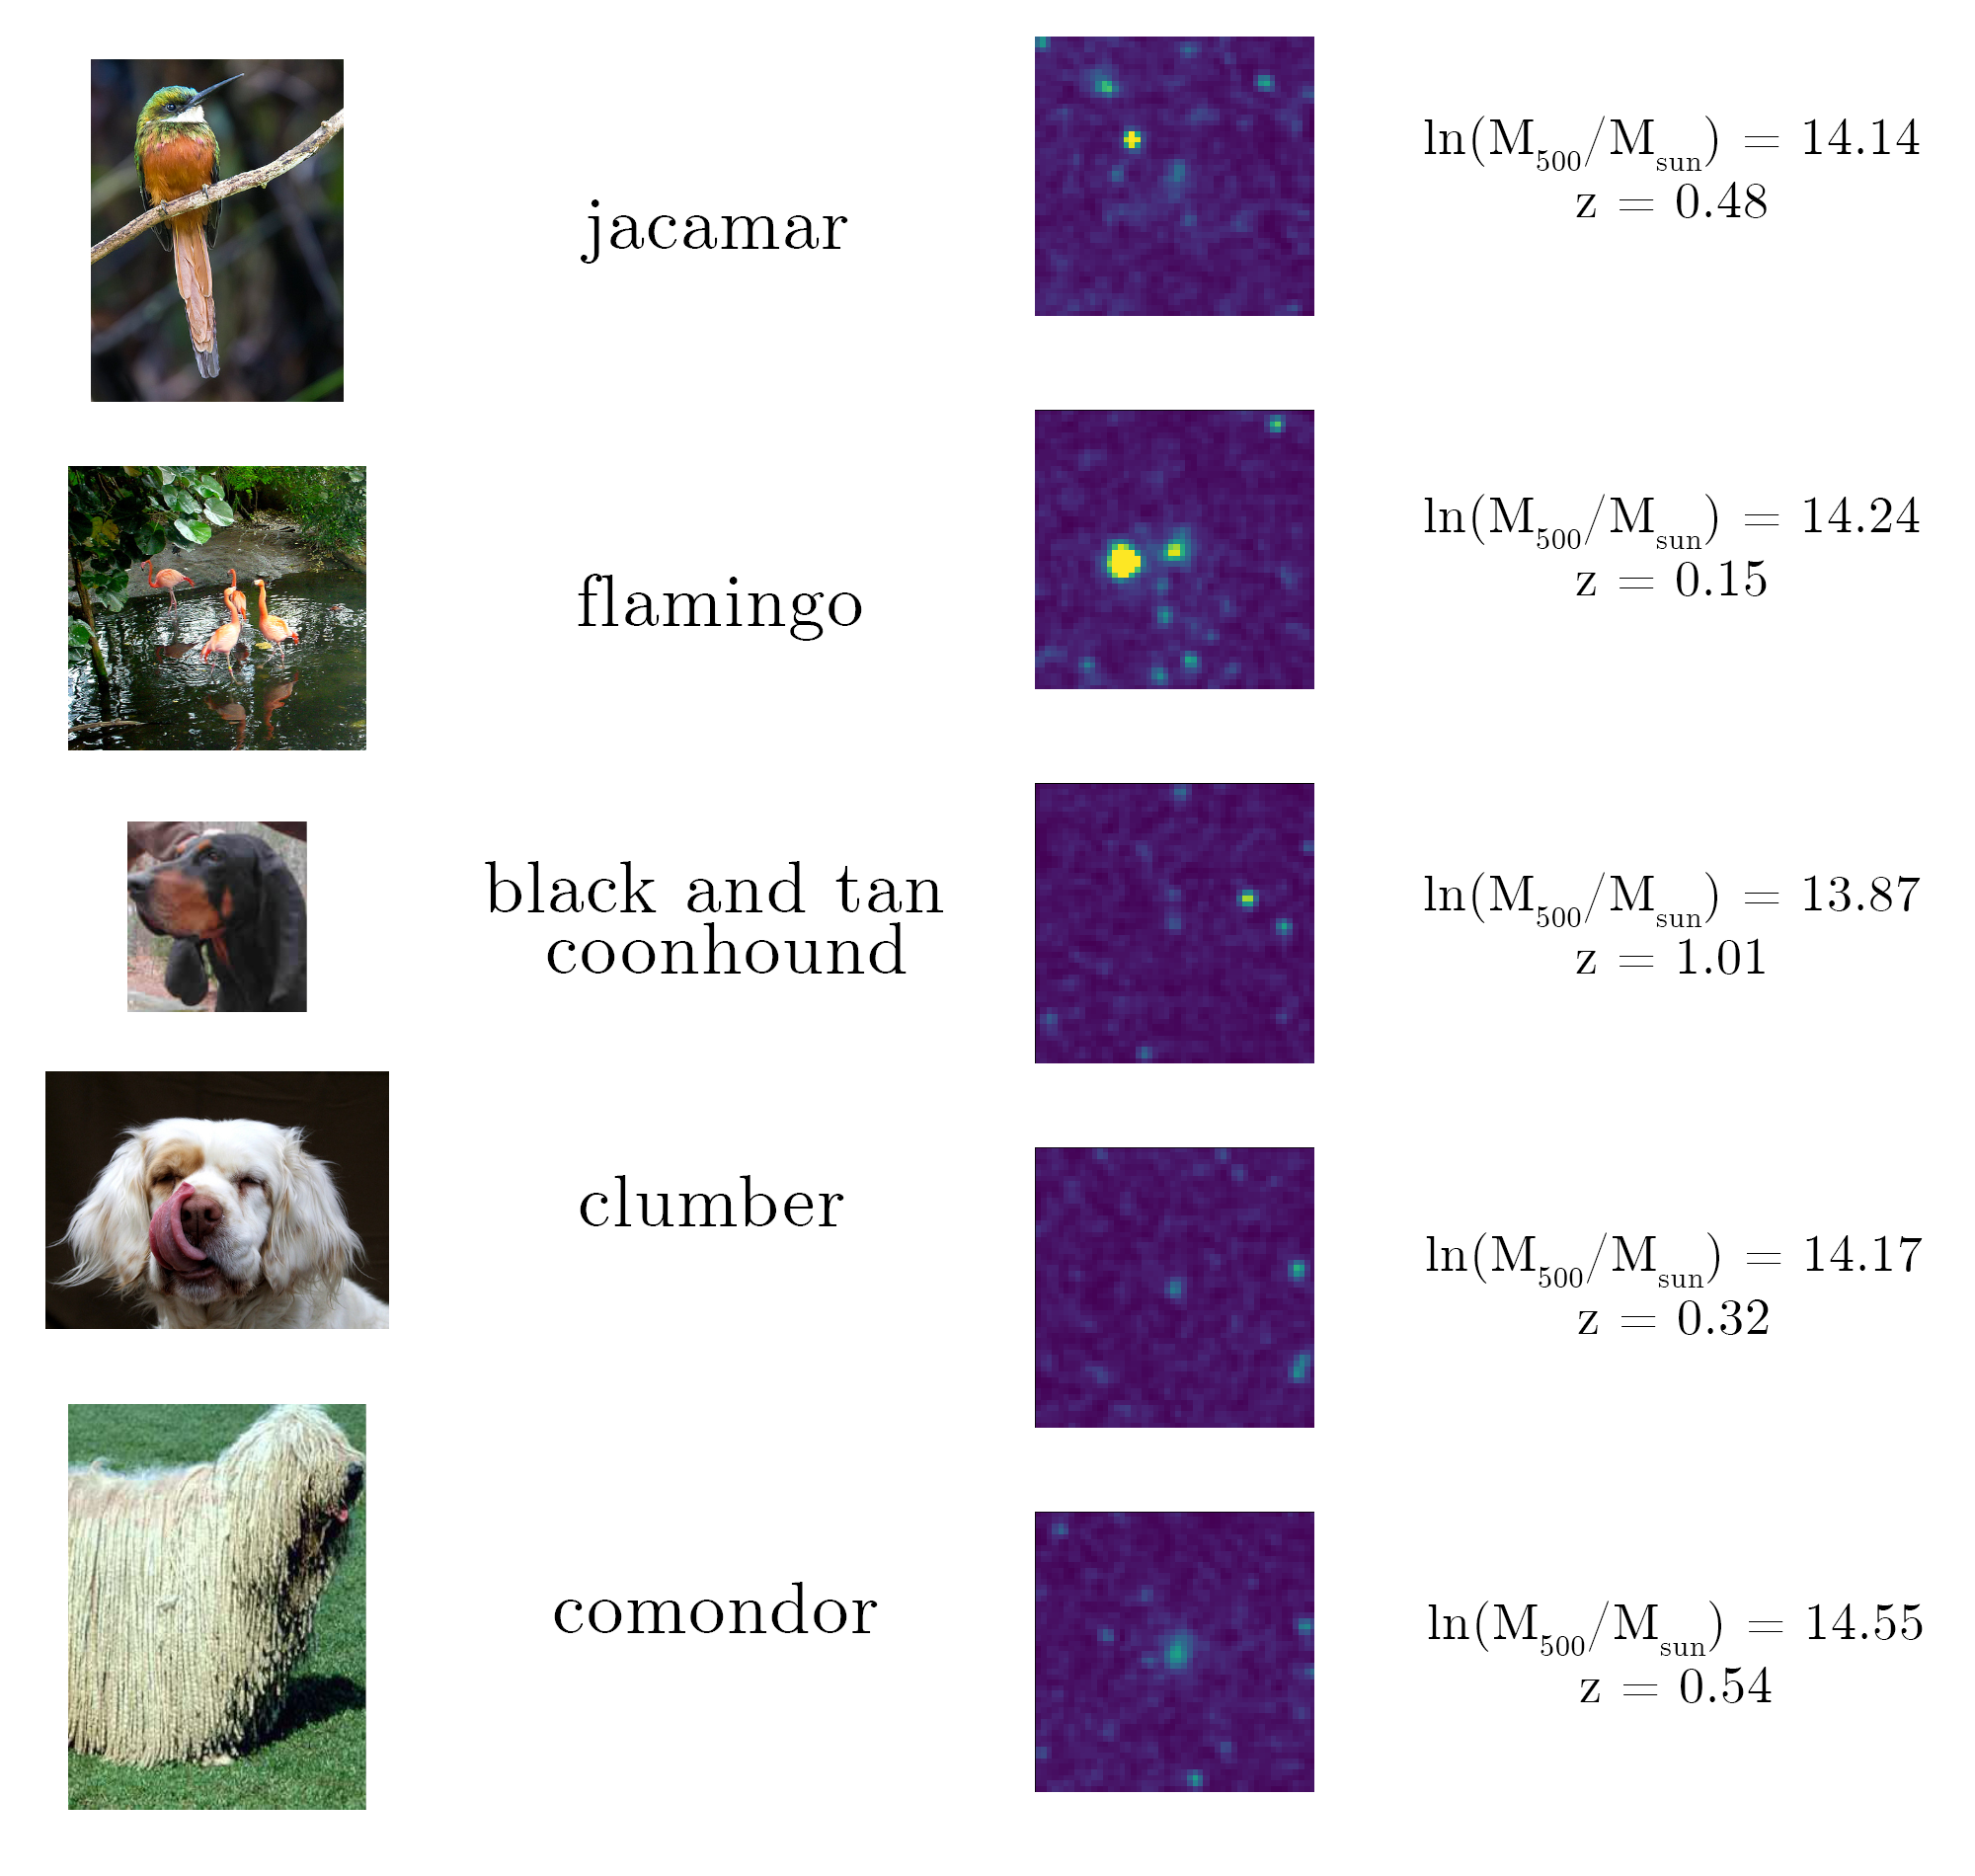
\includegraphics[width=0.8\textwidth]{images/Chapter2/imagenet_clusters.png}
 \caption{(\textit{Left}) images from ImageNet catalogue with labels (credit: ImageNet). (\textit{Right}) galaxy clusters from eFEDS simulation with mass and redshift as labels.}
 \label{fig:imagenet_clusters}
\end{figure}

The next plot shows the architectures of VGG19 and the shallower ResNet34 residual neural network.


\begin{figure}[H]
\centering
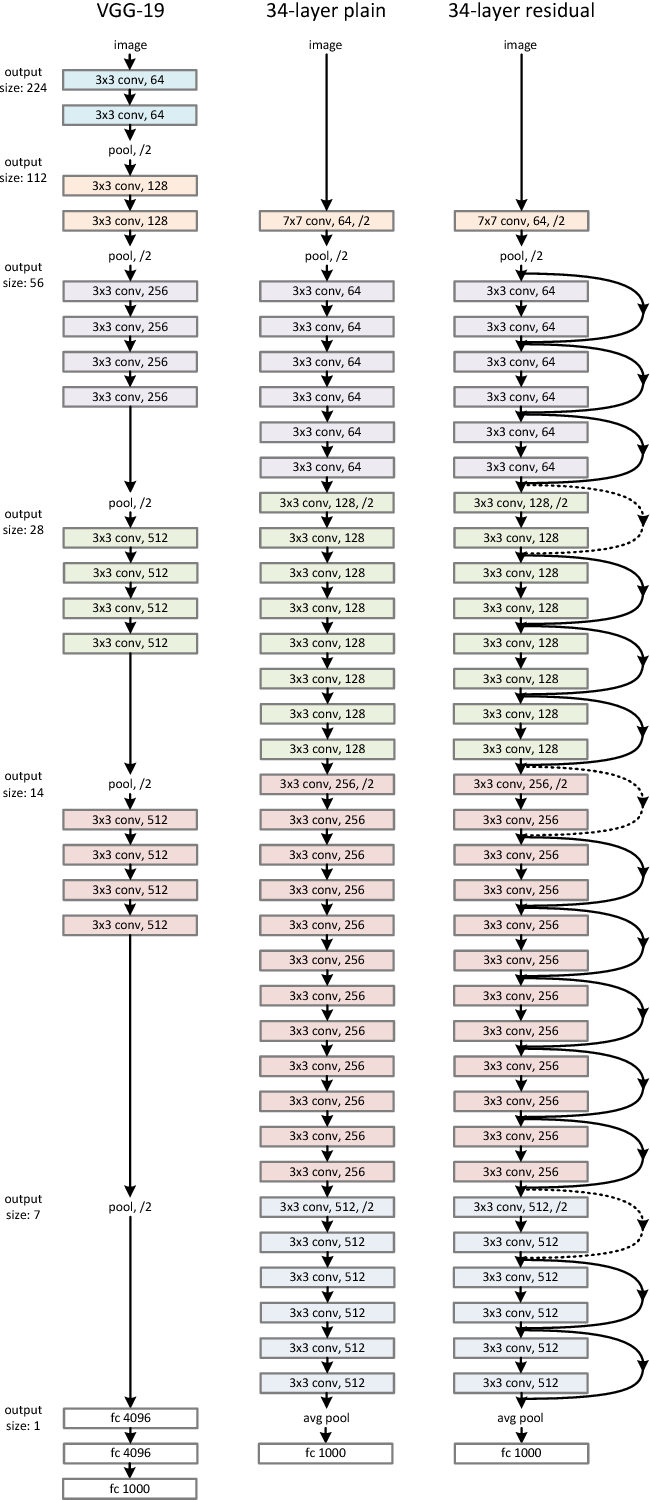
\includegraphics[width=.55\textwidth]{images/Chapter2/4-Figure3-1.png}
\caption{Comparison between VGG16's and ResNet's architecture.} 
\label{fig:Res34}
\end{figure} 

Finally, here are all the comparing results of the best deep models with the baseline model on the test and training set.


\begin{figure}[H]
\centering
\begin{subfigure}{.325\textwidth}
    \centering
    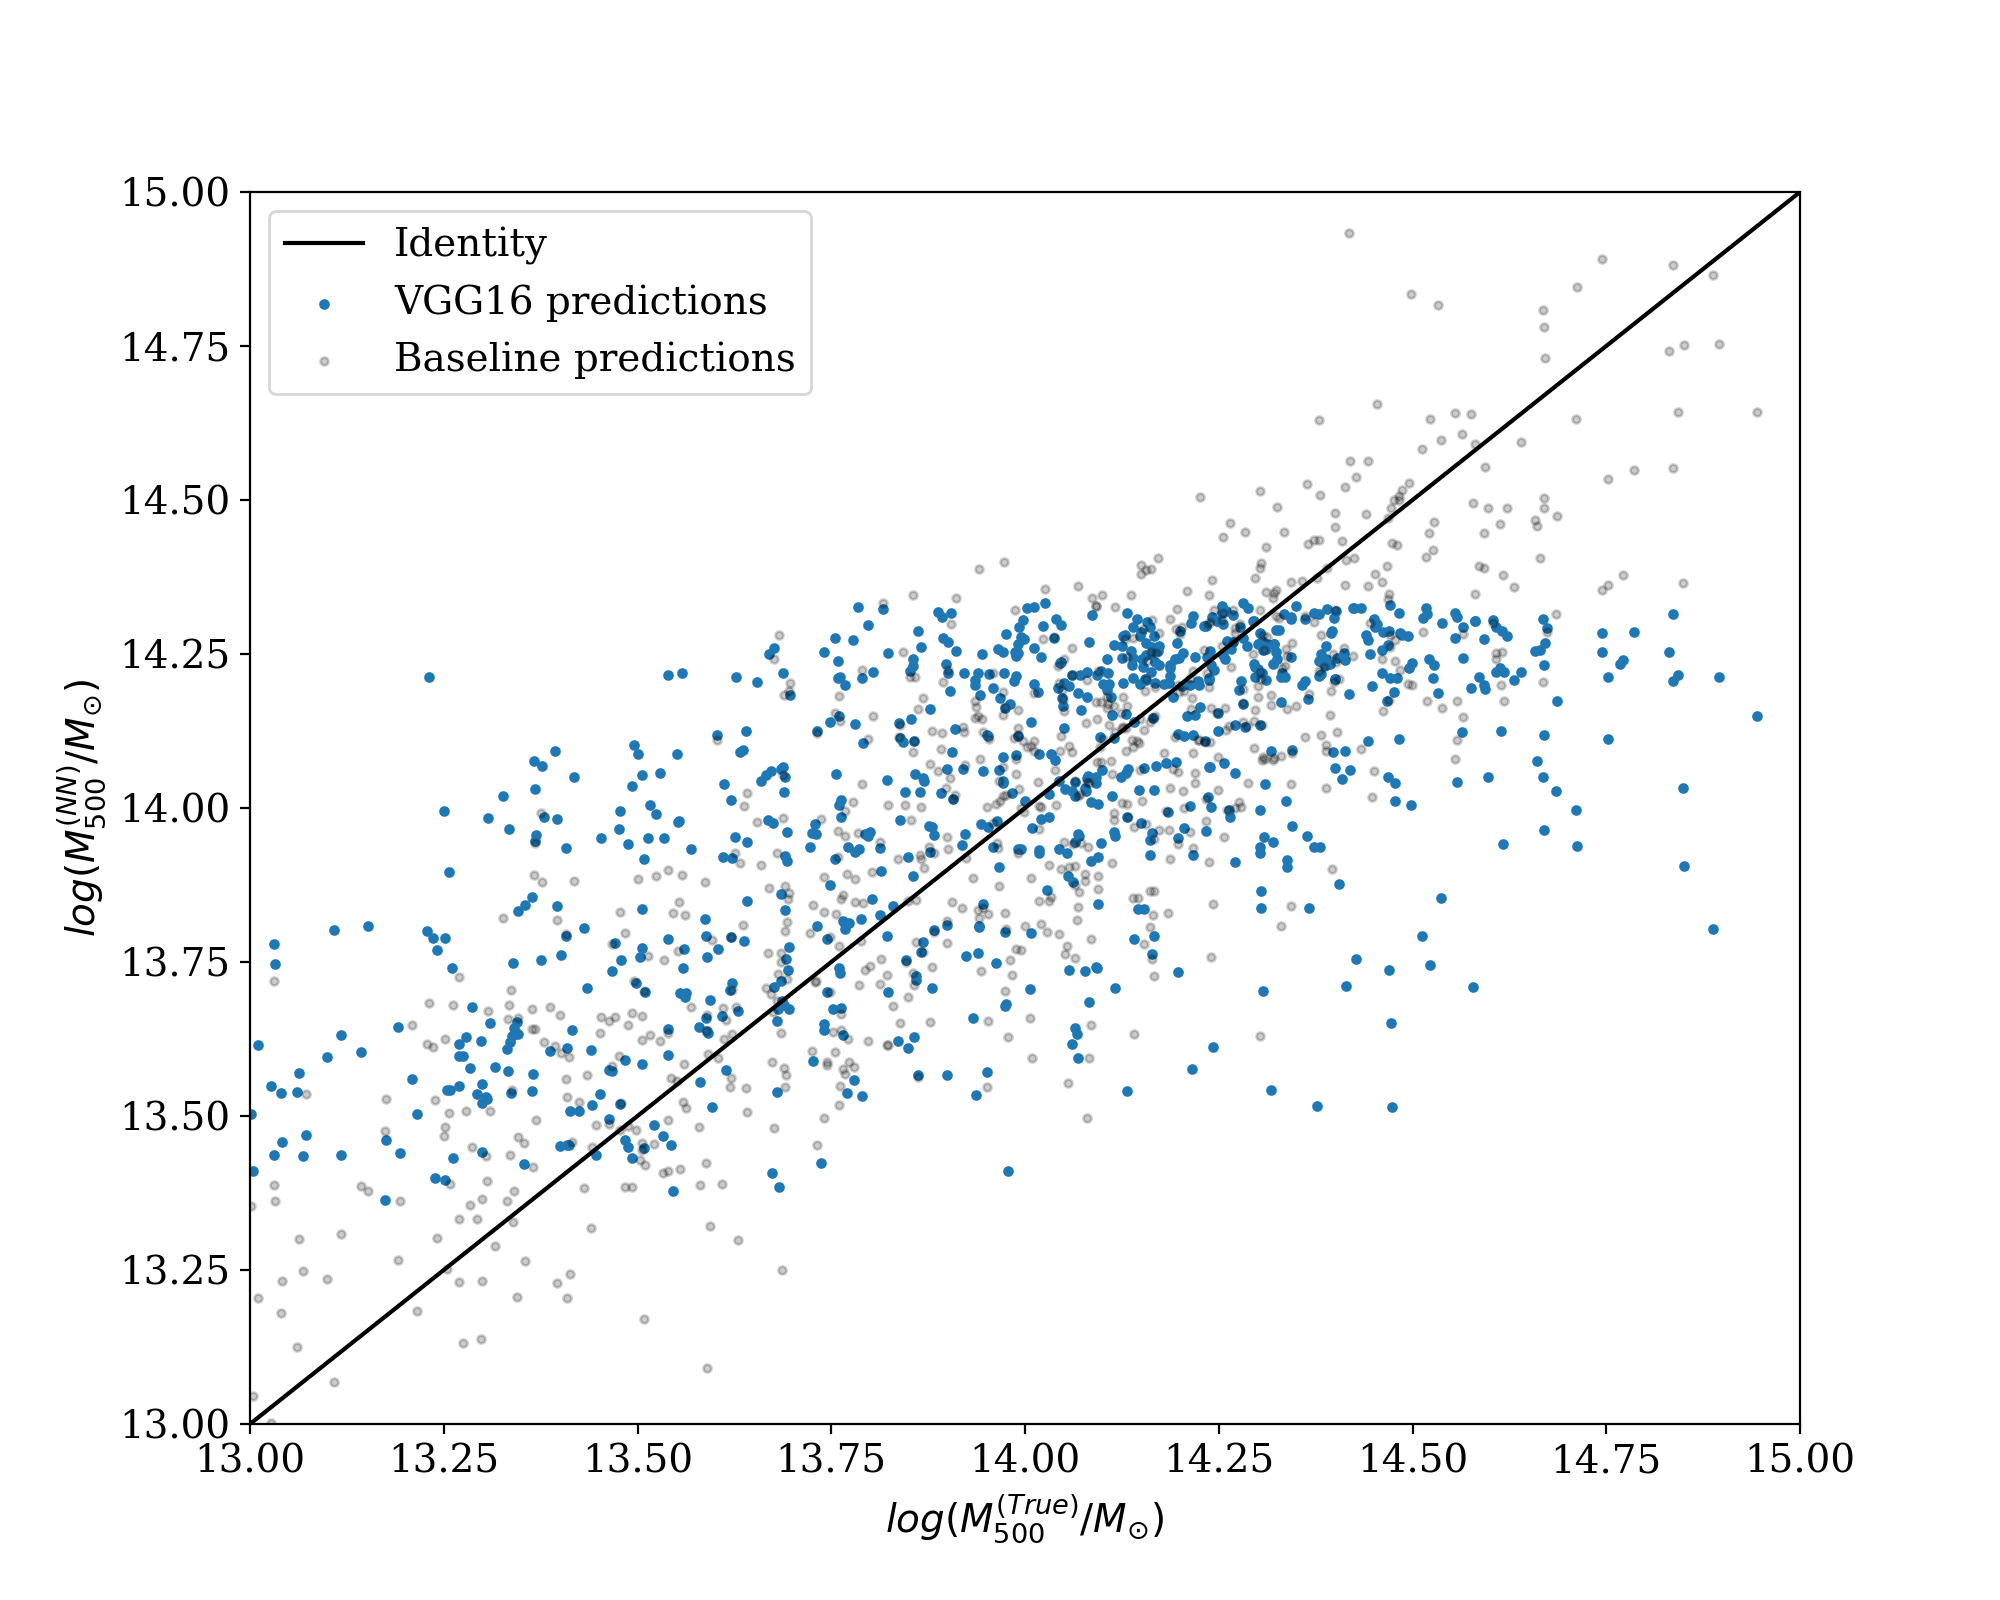
\includegraphics[width=\linewidth]{images/Chapter4/Results/test_VGG16_scatter.png}
    \label{fig:test_VGG16_scatter}
    \caption{VGG16}
\end{subfigure}
\begin{subfigure}{.325\textwidth}
    \centering
    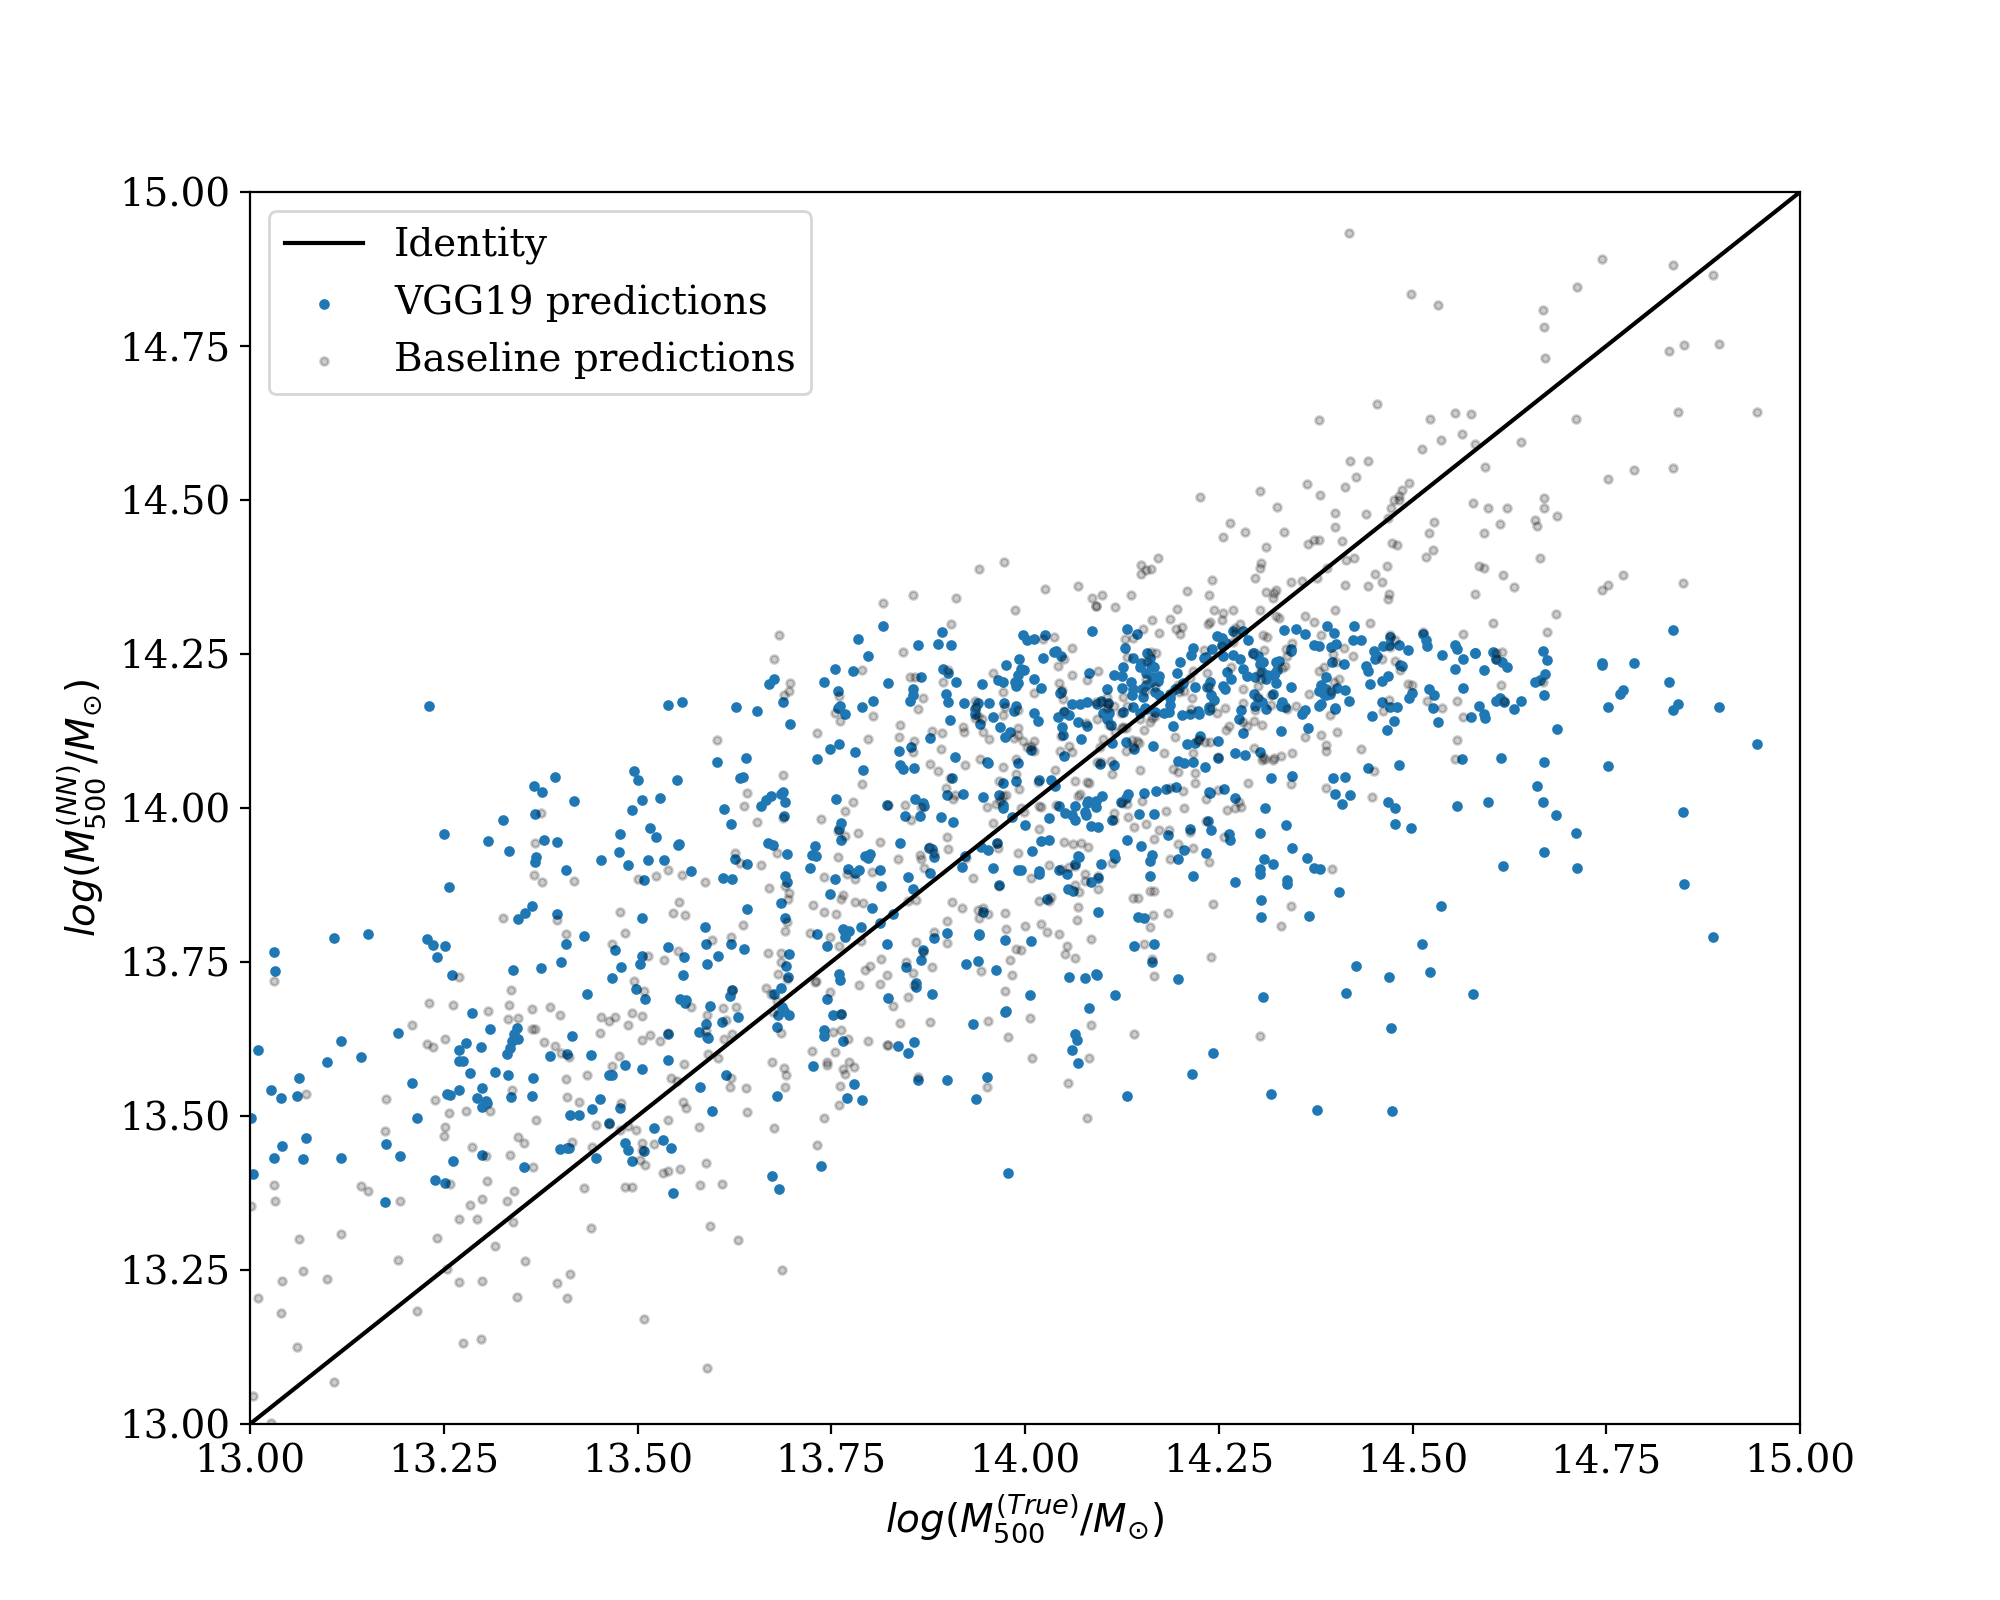
\includegraphics[width=\linewidth]{images/Chapter4/Results/test_VGG19_scatter.png}
    \label{fig:test_VGG19_scatter}
    \caption{VGG19}
\end{subfigure}
\begin{subfigure}{.325\textwidth}
    \centering
    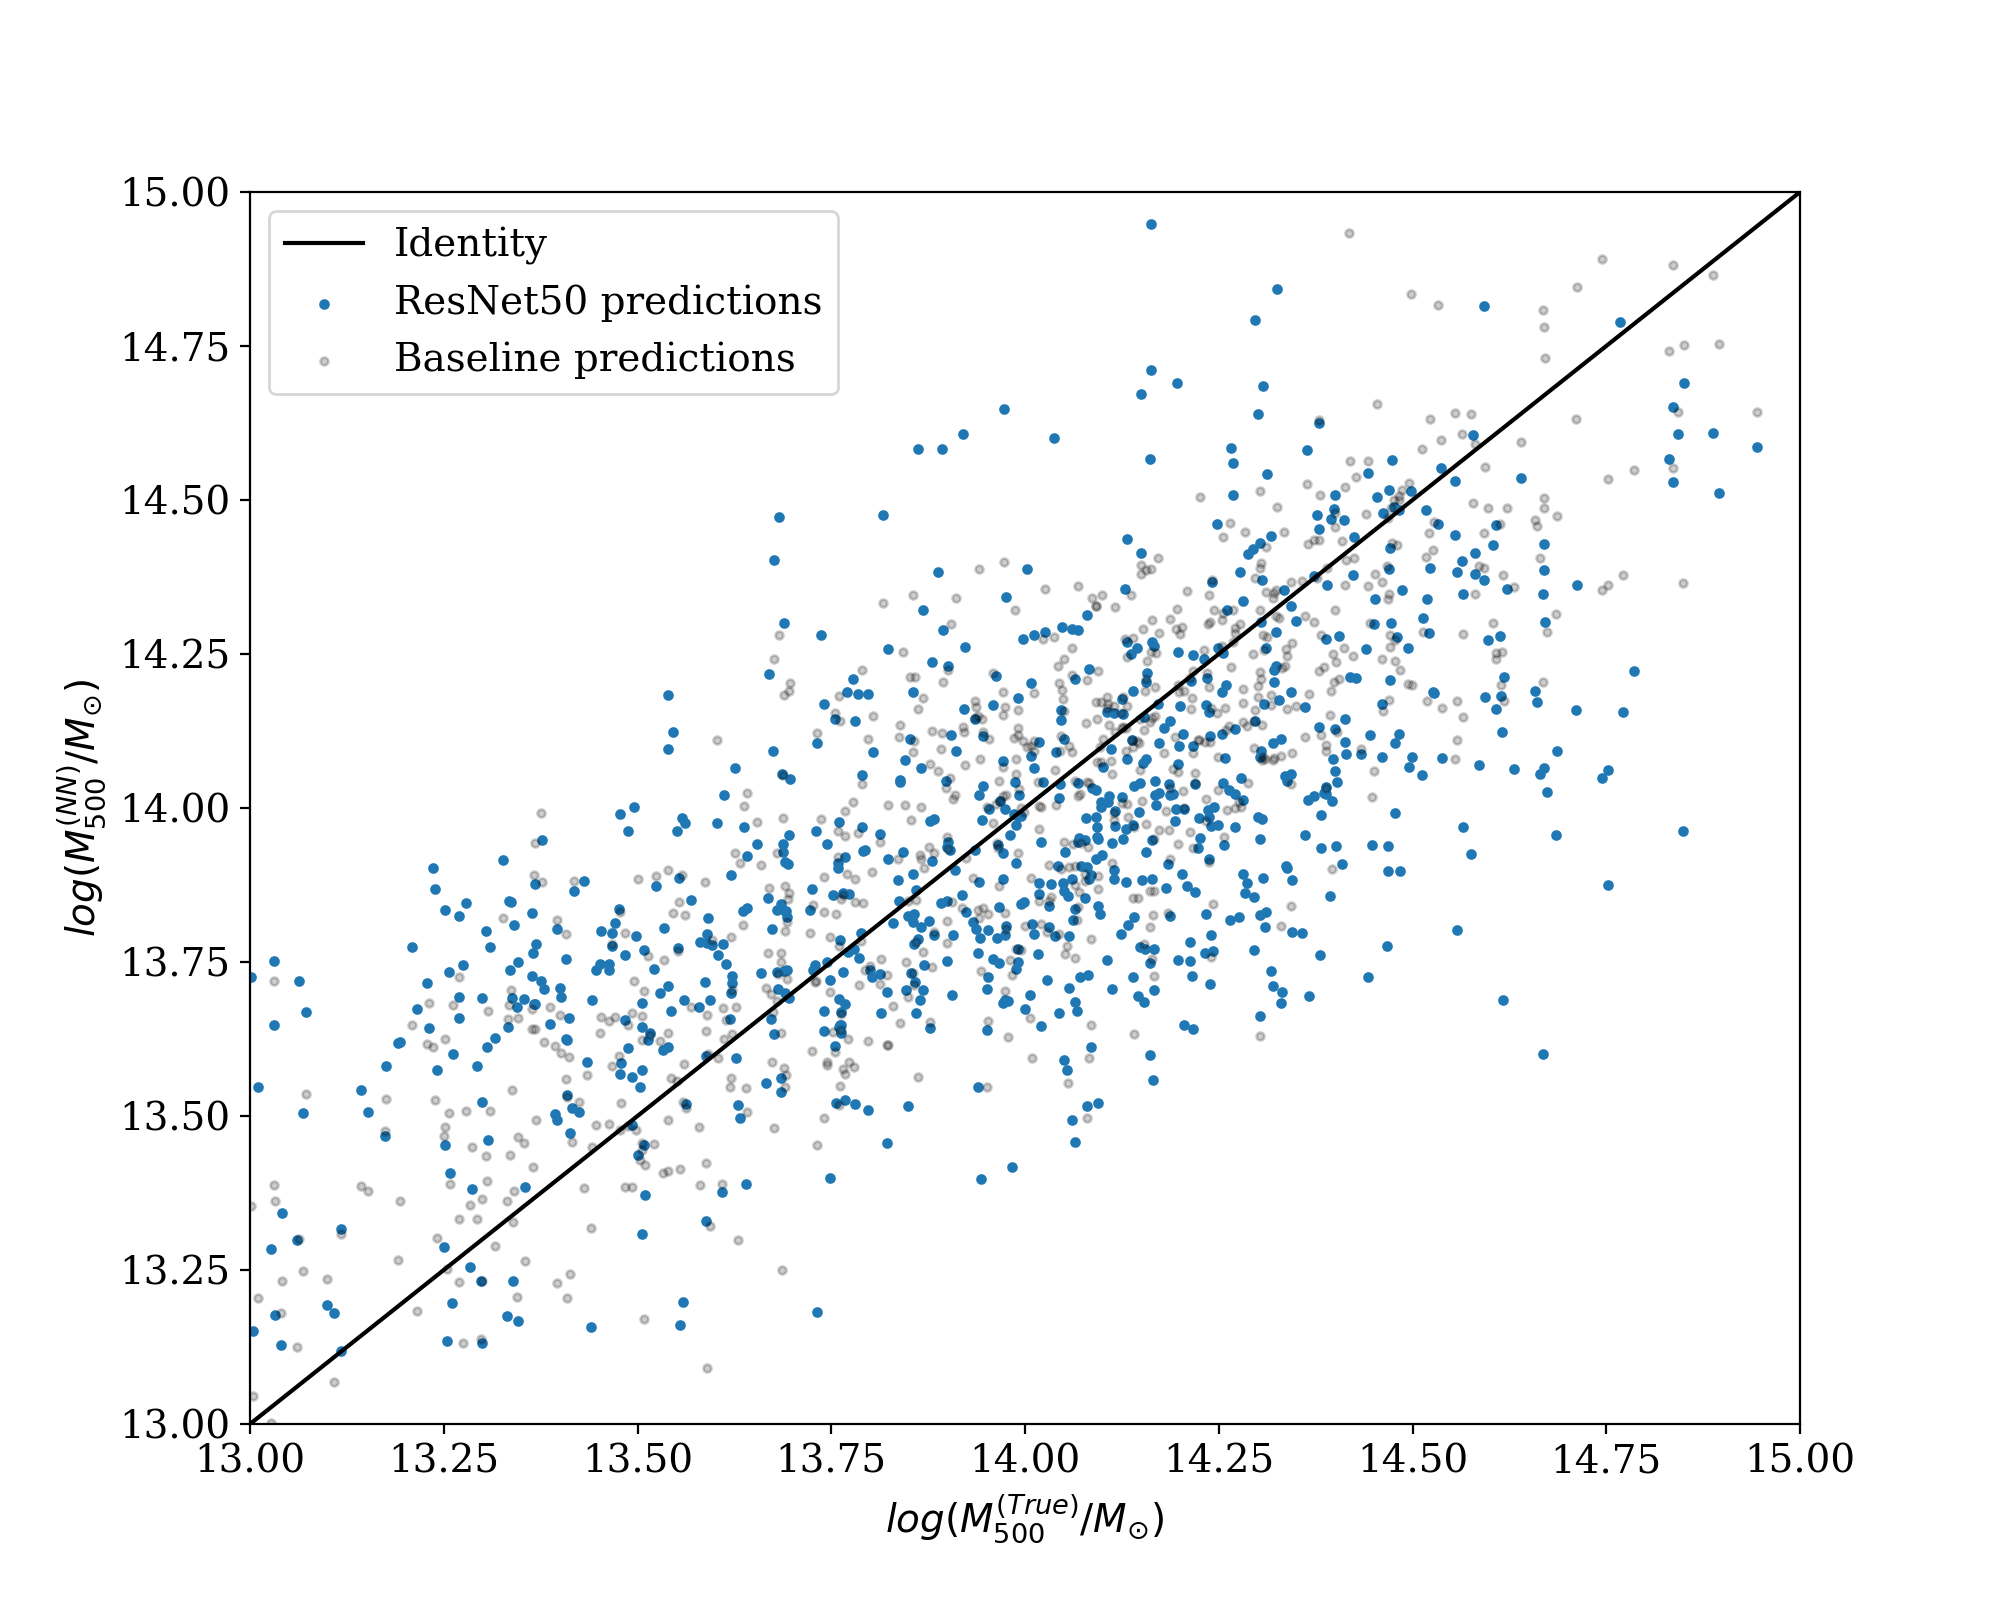
\includegraphics[width=\linewidth]{images/Chapter4/Results/test_ResNet50_scatter.png}
    \label{fig:test_ResNet50_scatter}
    \caption{ResNet50}
\end{subfigure}
\begin{subfigure}{.325\textwidth}
    \centering
    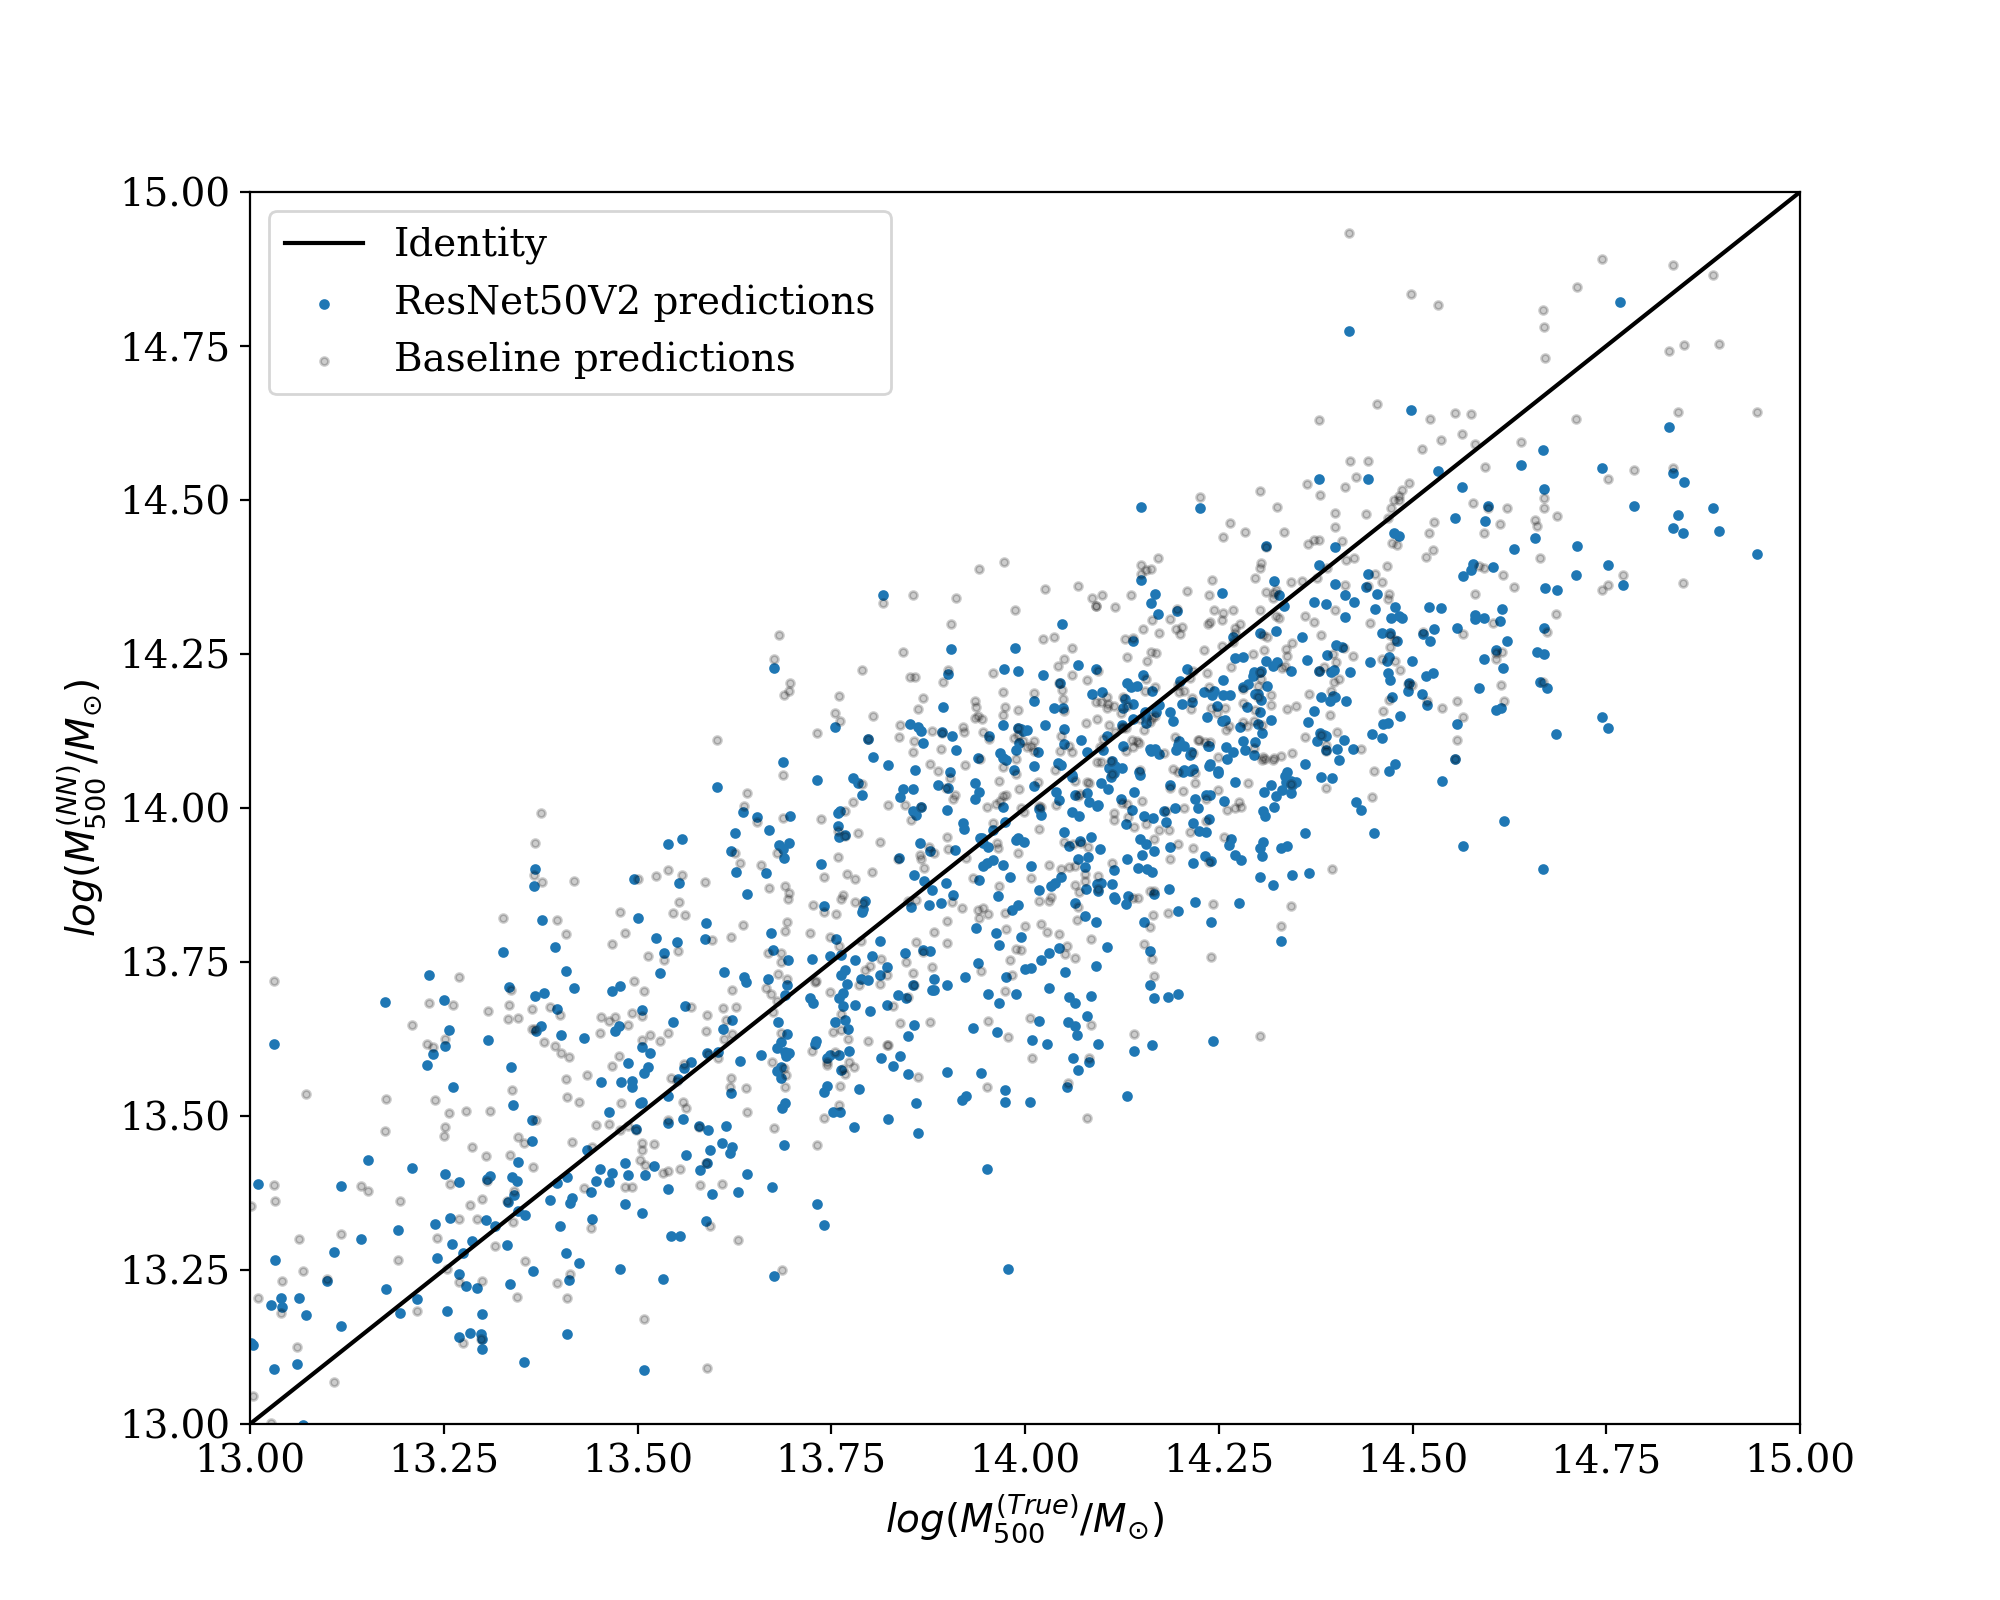
\includegraphics[width=\linewidth]{images/Chapter4/Results/test_ResNet50V2_scatter.png}
    \label{fig:test_ResNet50V2_scatter}
    \caption{ResNet50V2}
\end{subfigure}
\begin{subfigure}{.325\textwidth}
    \centering
    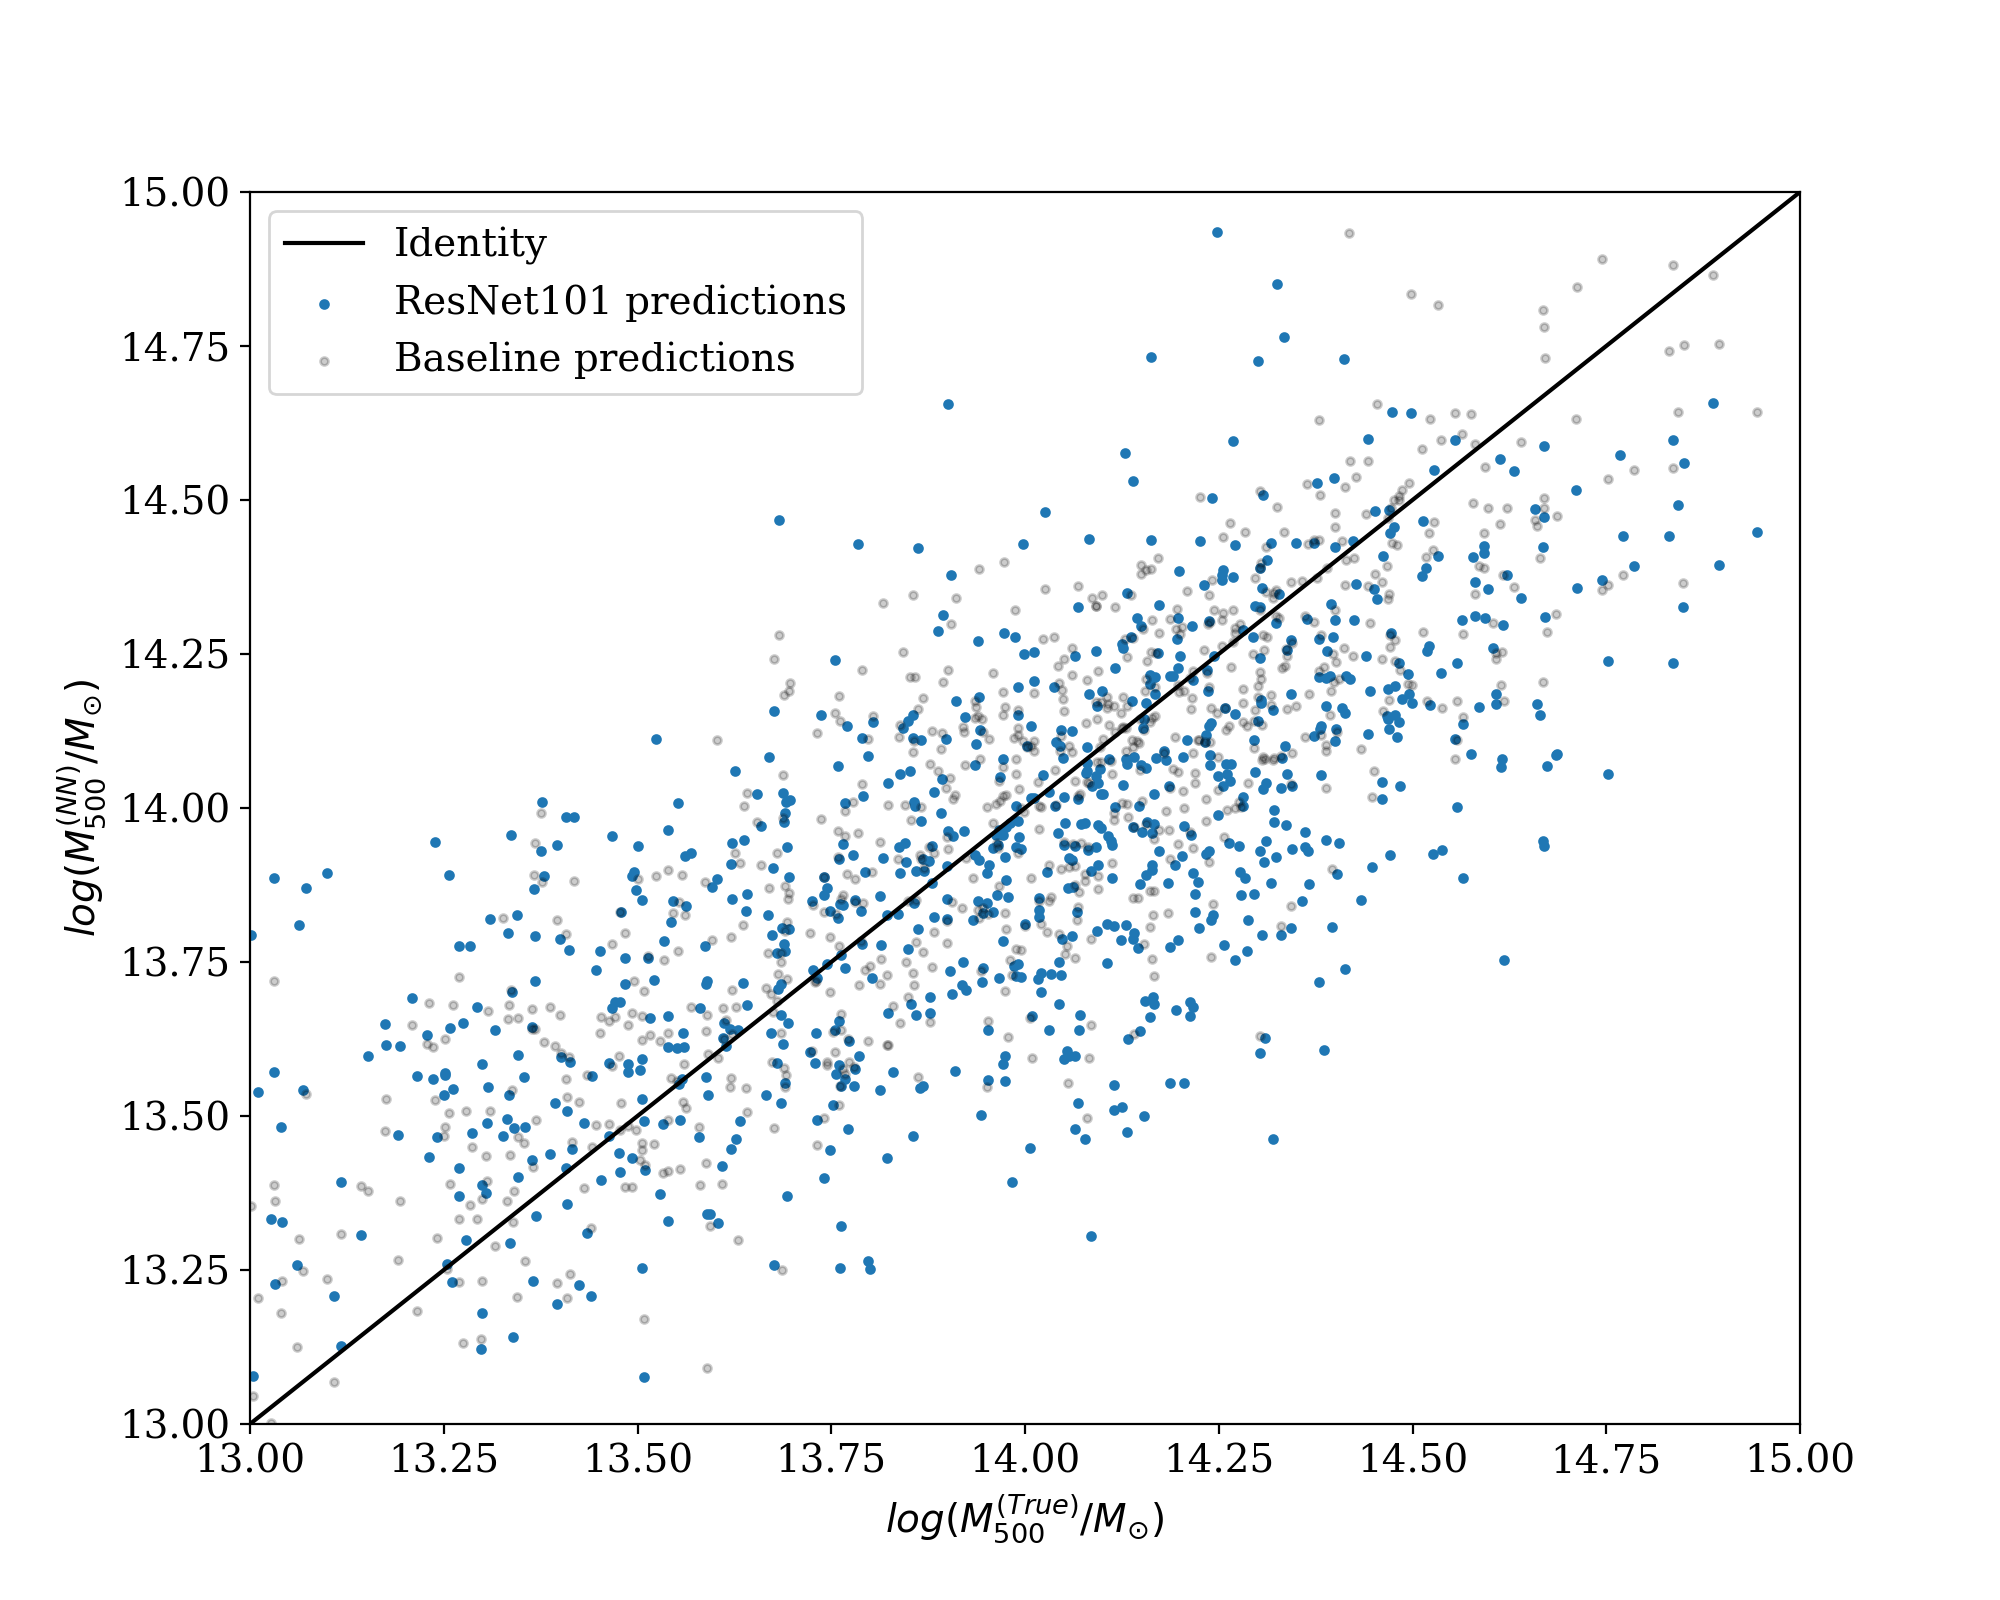
\includegraphics[width=\linewidth]{images/Chapter4/Results/test_ResNet101_scatter.png}
    \label{fig:test_ResNet101_scatter}
    \caption{ResNet101}
\end{subfigure}
\begin{subfigure}{.325\textwidth}
    \centering
    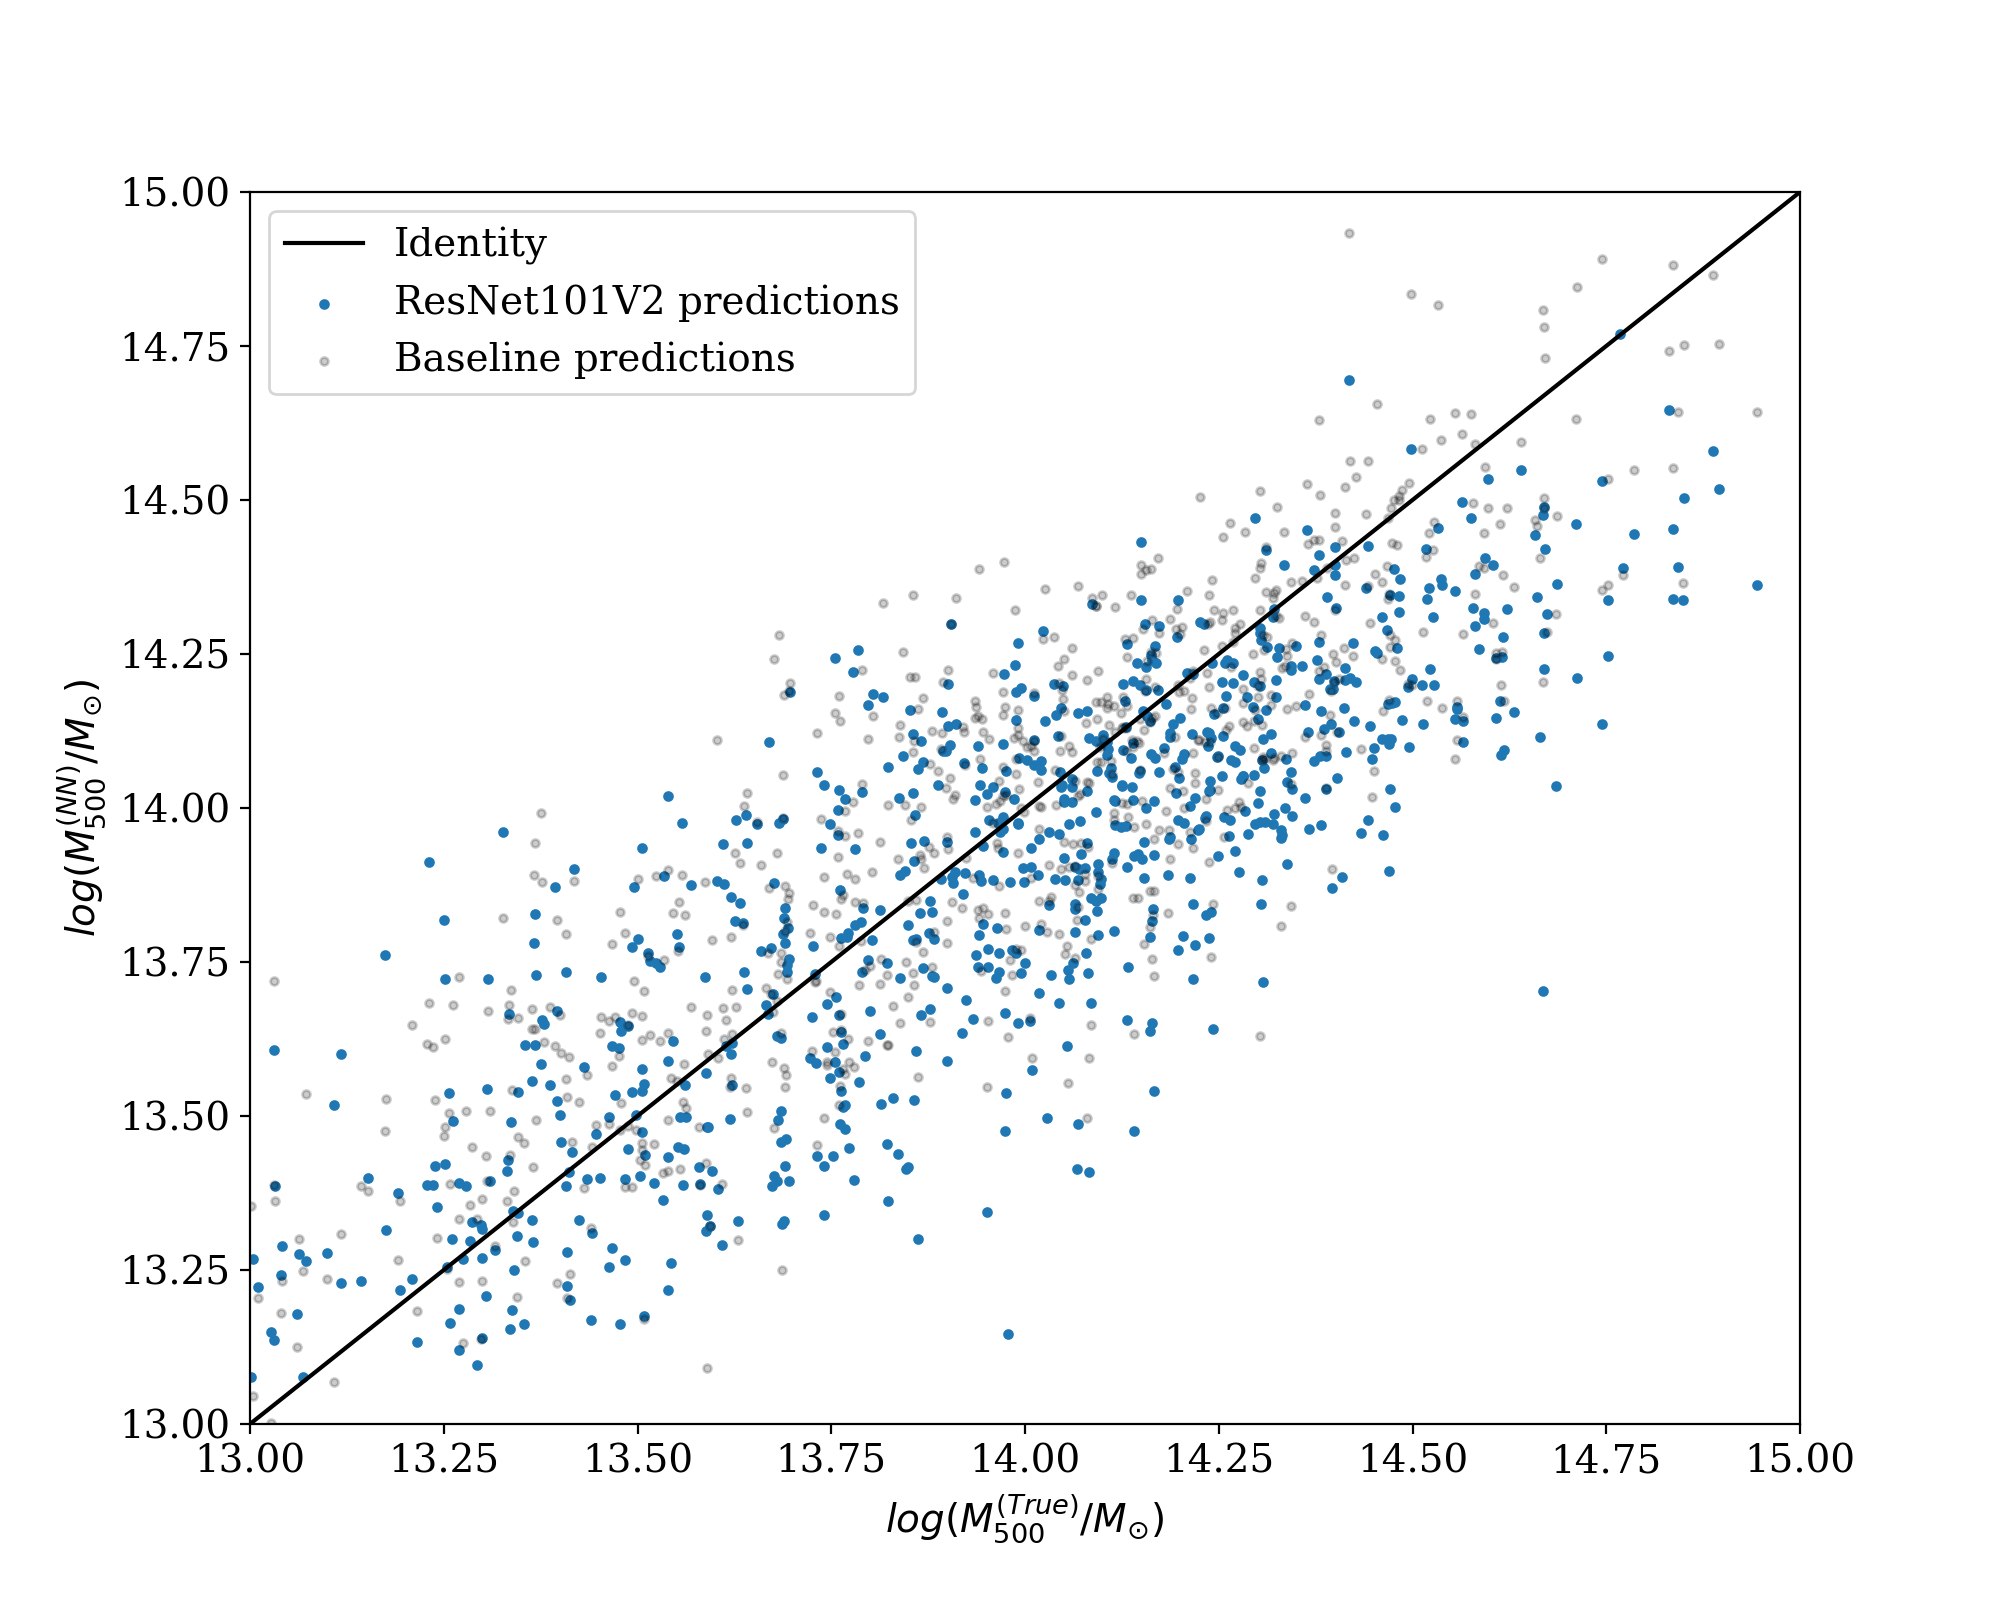
\includegraphics[width=\linewidth]{images/Chapter4/Results/test_ResNet101V2_scatter.png}
    \label{fig:test_ResNet101V2_scatter}
    \caption{ResNet101V2}
\end{subfigure}
\begin{subfigure}{.325\textwidth}
    \centering
    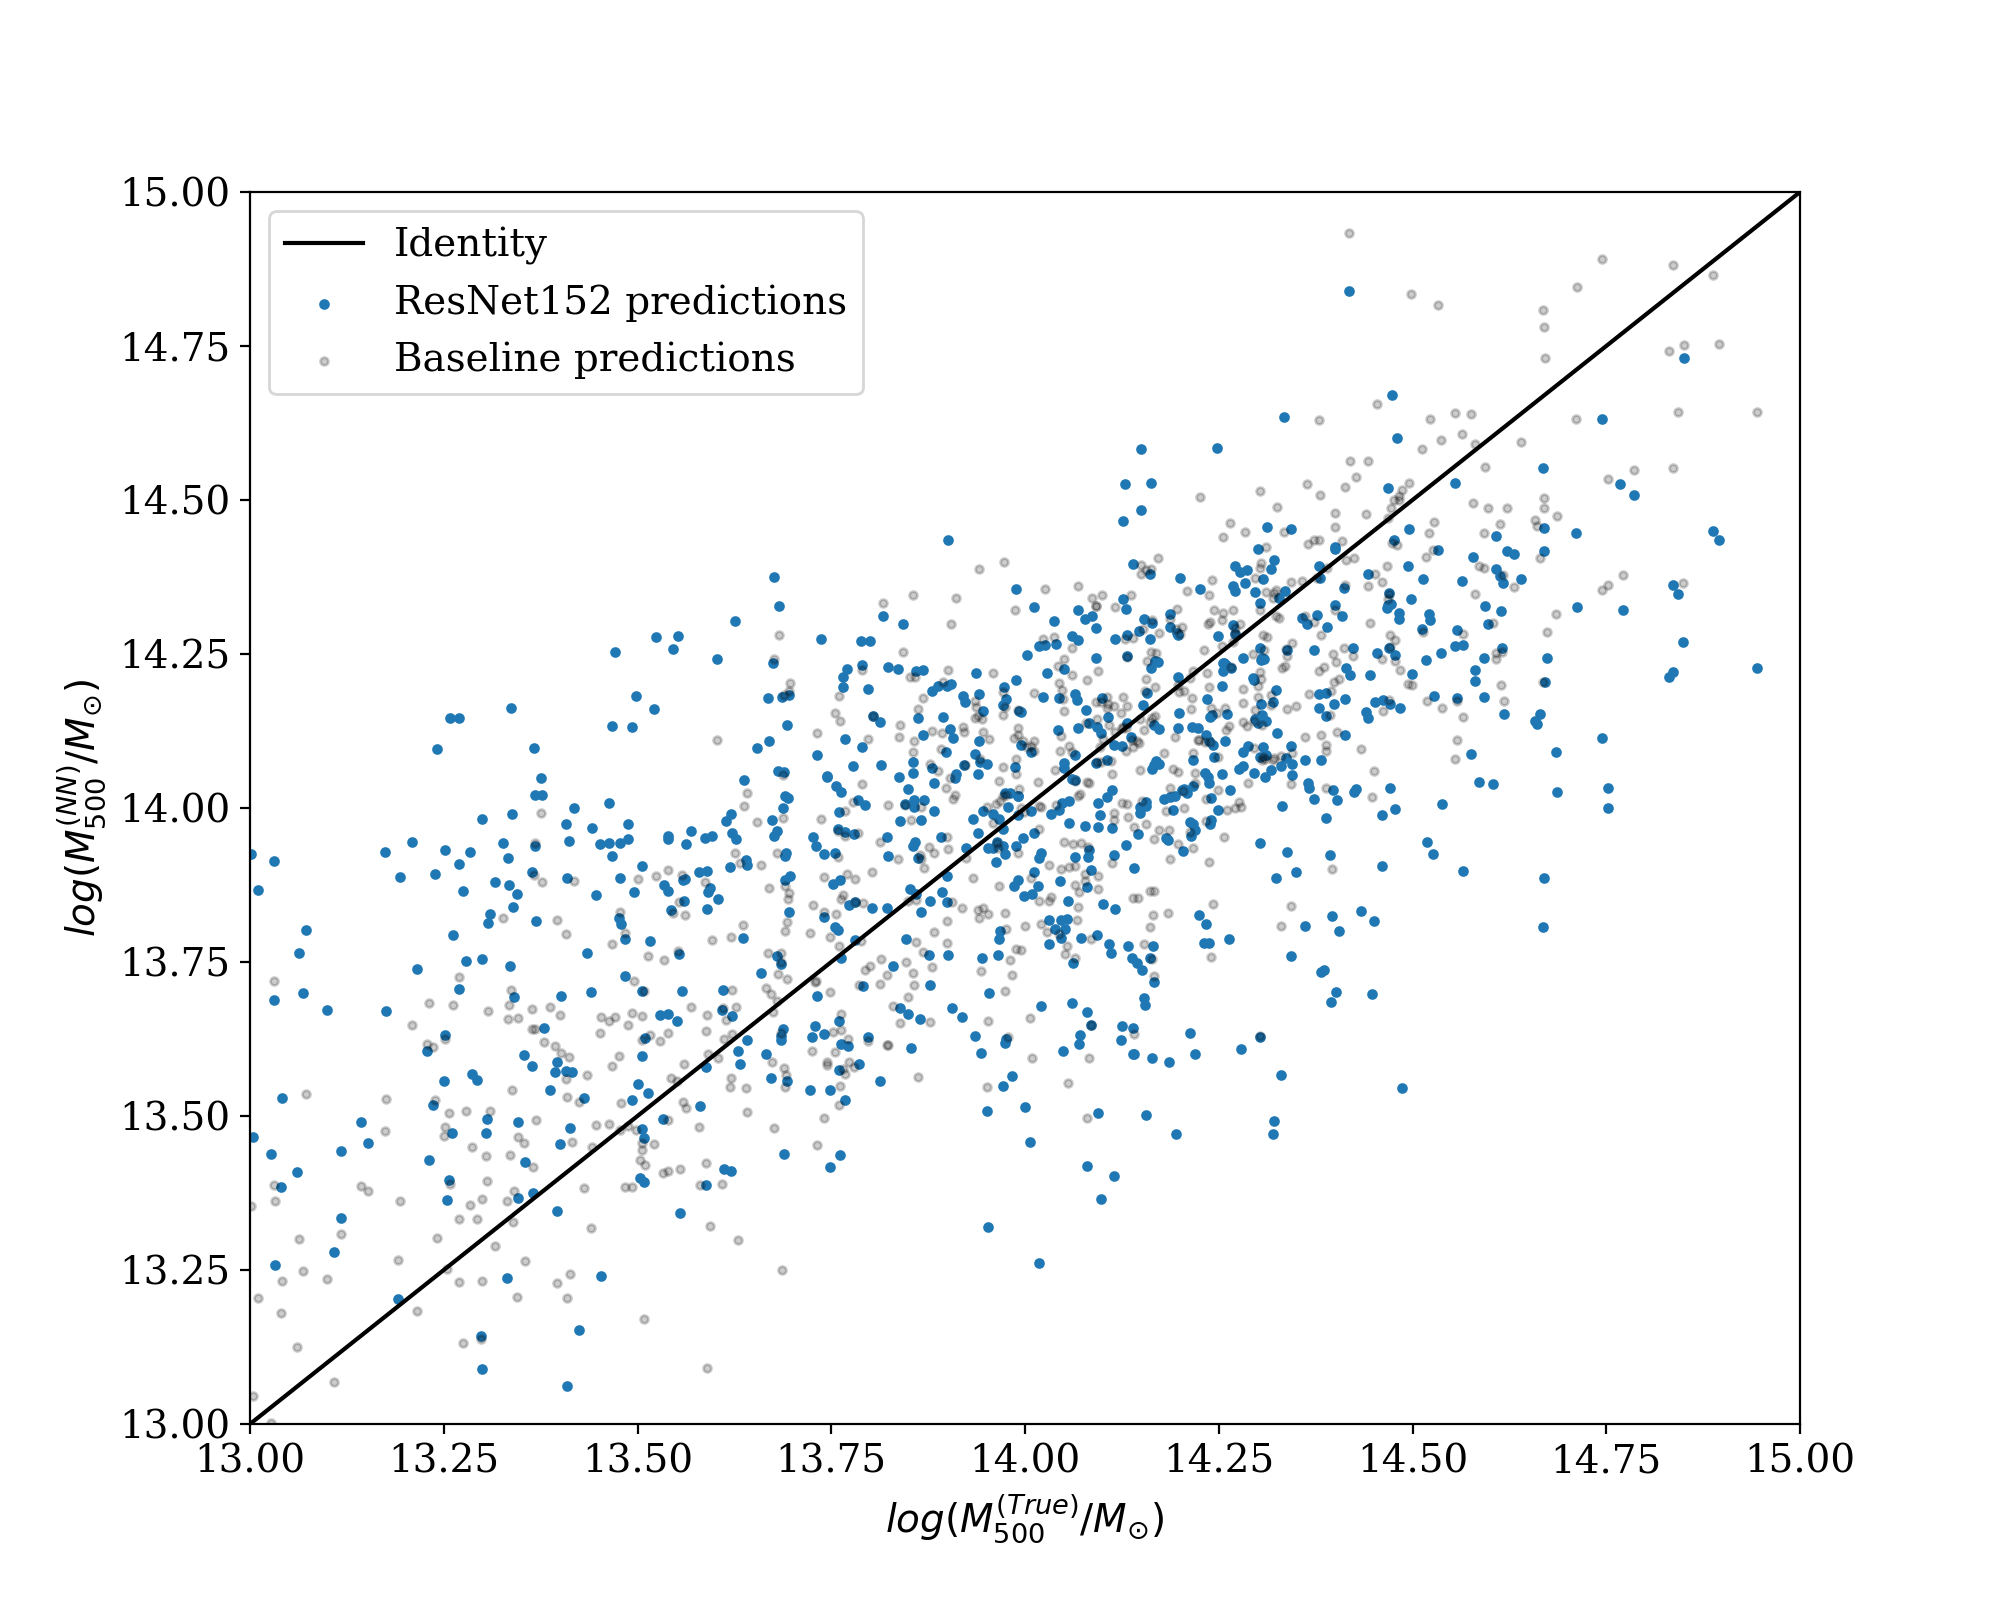
\includegraphics[width=\linewidth]{images/Chapter4/Results/test_ResNet152_scatter.png}
    \label{fig:test_ResNet152_scatter}
    \caption{ResNet152}
\end{subfigure}
\begin{subfigure}{.325\textwidth}
    \centering
    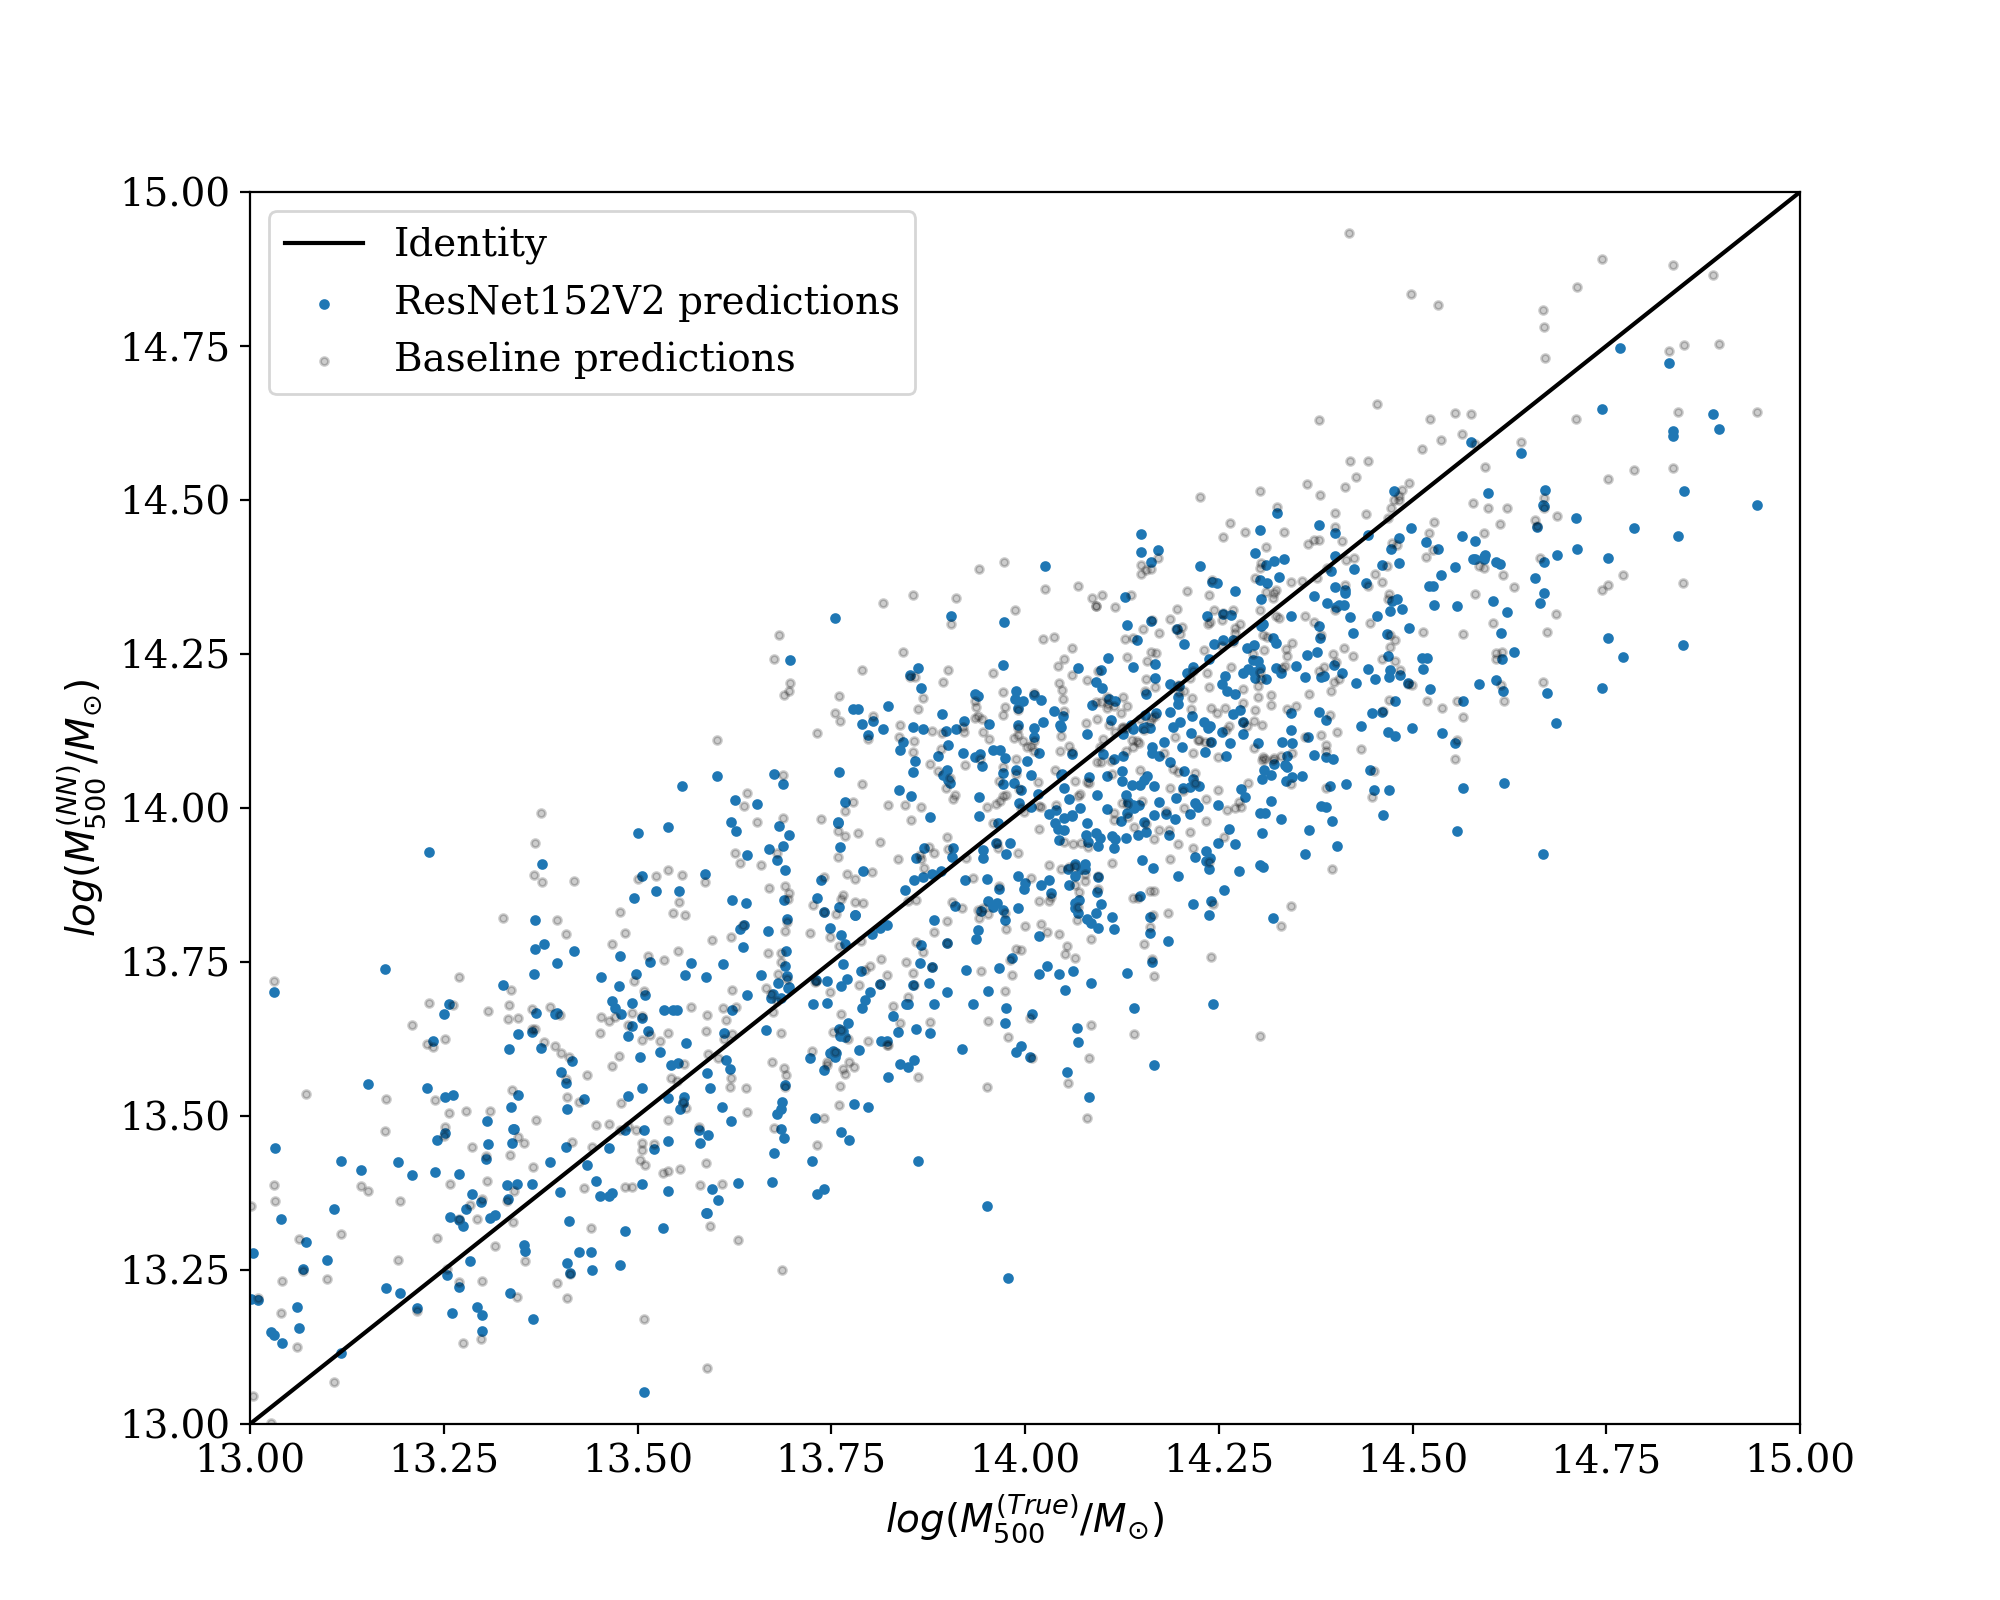
\includegraphics[width=\linewidth]{images/Chapter4/Results/test_ResNet152V2_scatter.png}
    \label{fig:test_ResNet152V2_scatter}
    \caption{ResNet152V2}
\end{subfigure}
\begin{subfigure}{.325\textwidth}
    \centering
    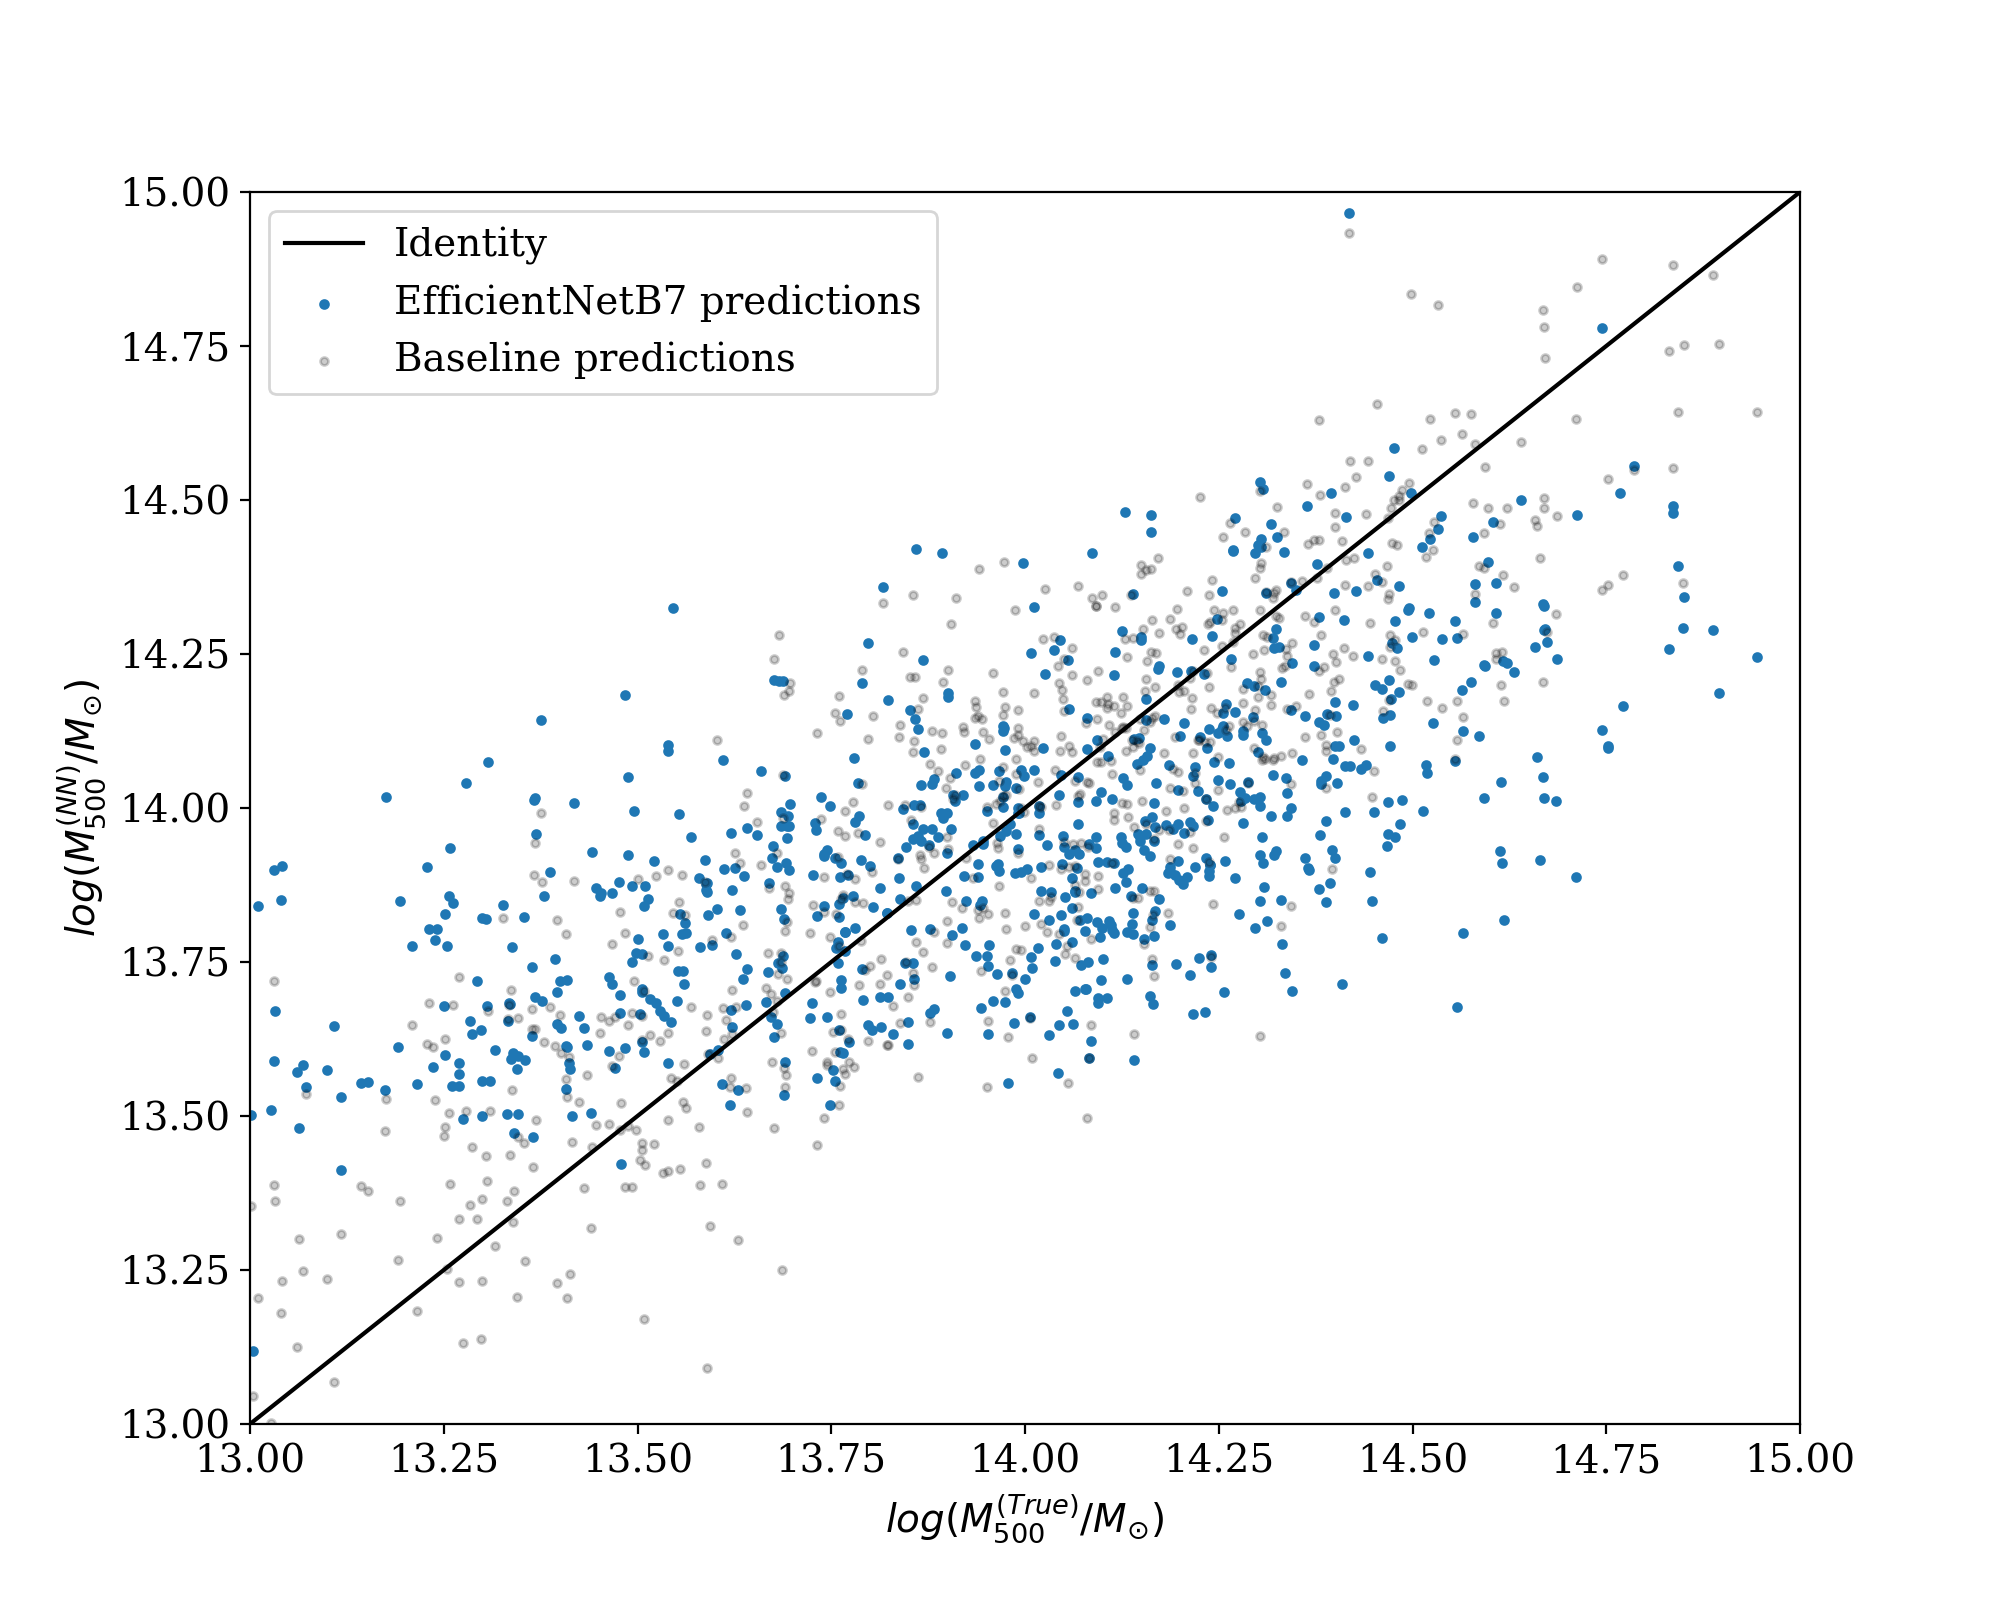
\includegraphics[width=\linewidth]{images/Chapter4/Results/test_EfficientNetB7_scatter.png}
    \label{fig:test_EfficientNetB7_scatter}
    \caption{EfficientNetB7}
\end{subfigure}
\caption{Comparison between each deep model's best predictions (\textit{blue}) and the best predictions from the basic CNN (\textit{grey}) in the test set.}
\end{figure}

\begin{figure}[H]
\centering
\begin{subfigure}{.325\textwidth}
    \centering
    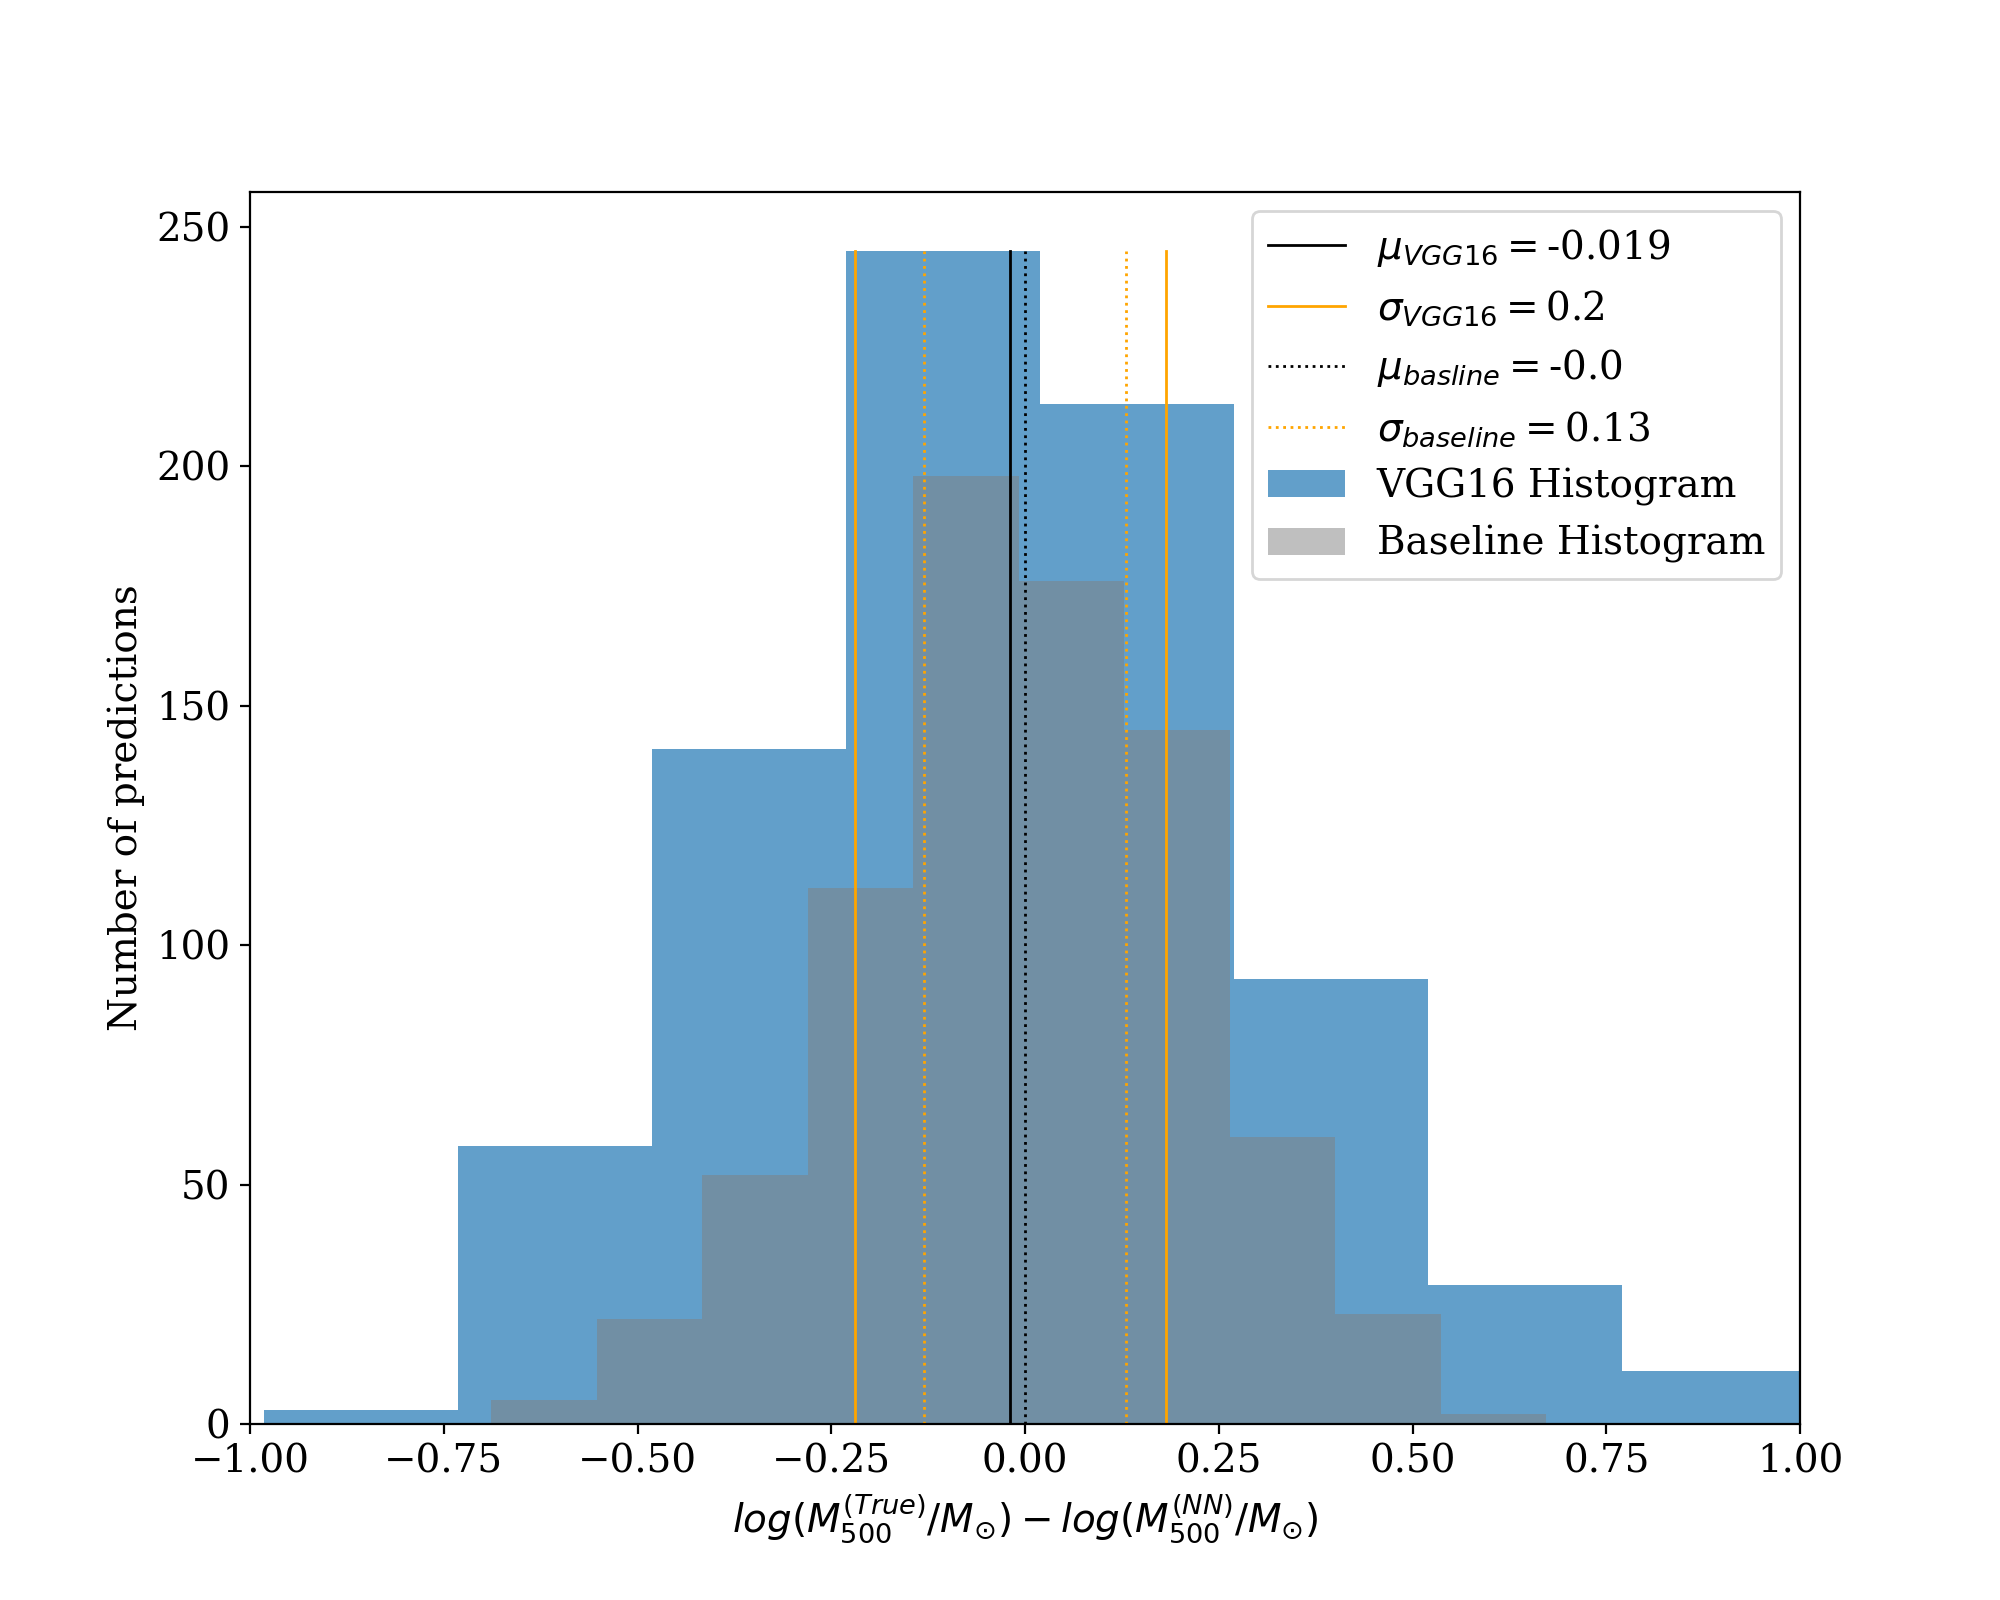
\includegraphics[width=\linewidth]{images/Chapter4/Results/test_VGG16_hist.png}
    \label{fig:test_VGG16_hist}
    \caption{VGG16}
\end{subfigure}
\begin{subfigure}{.325\textwidth}
    \centering
    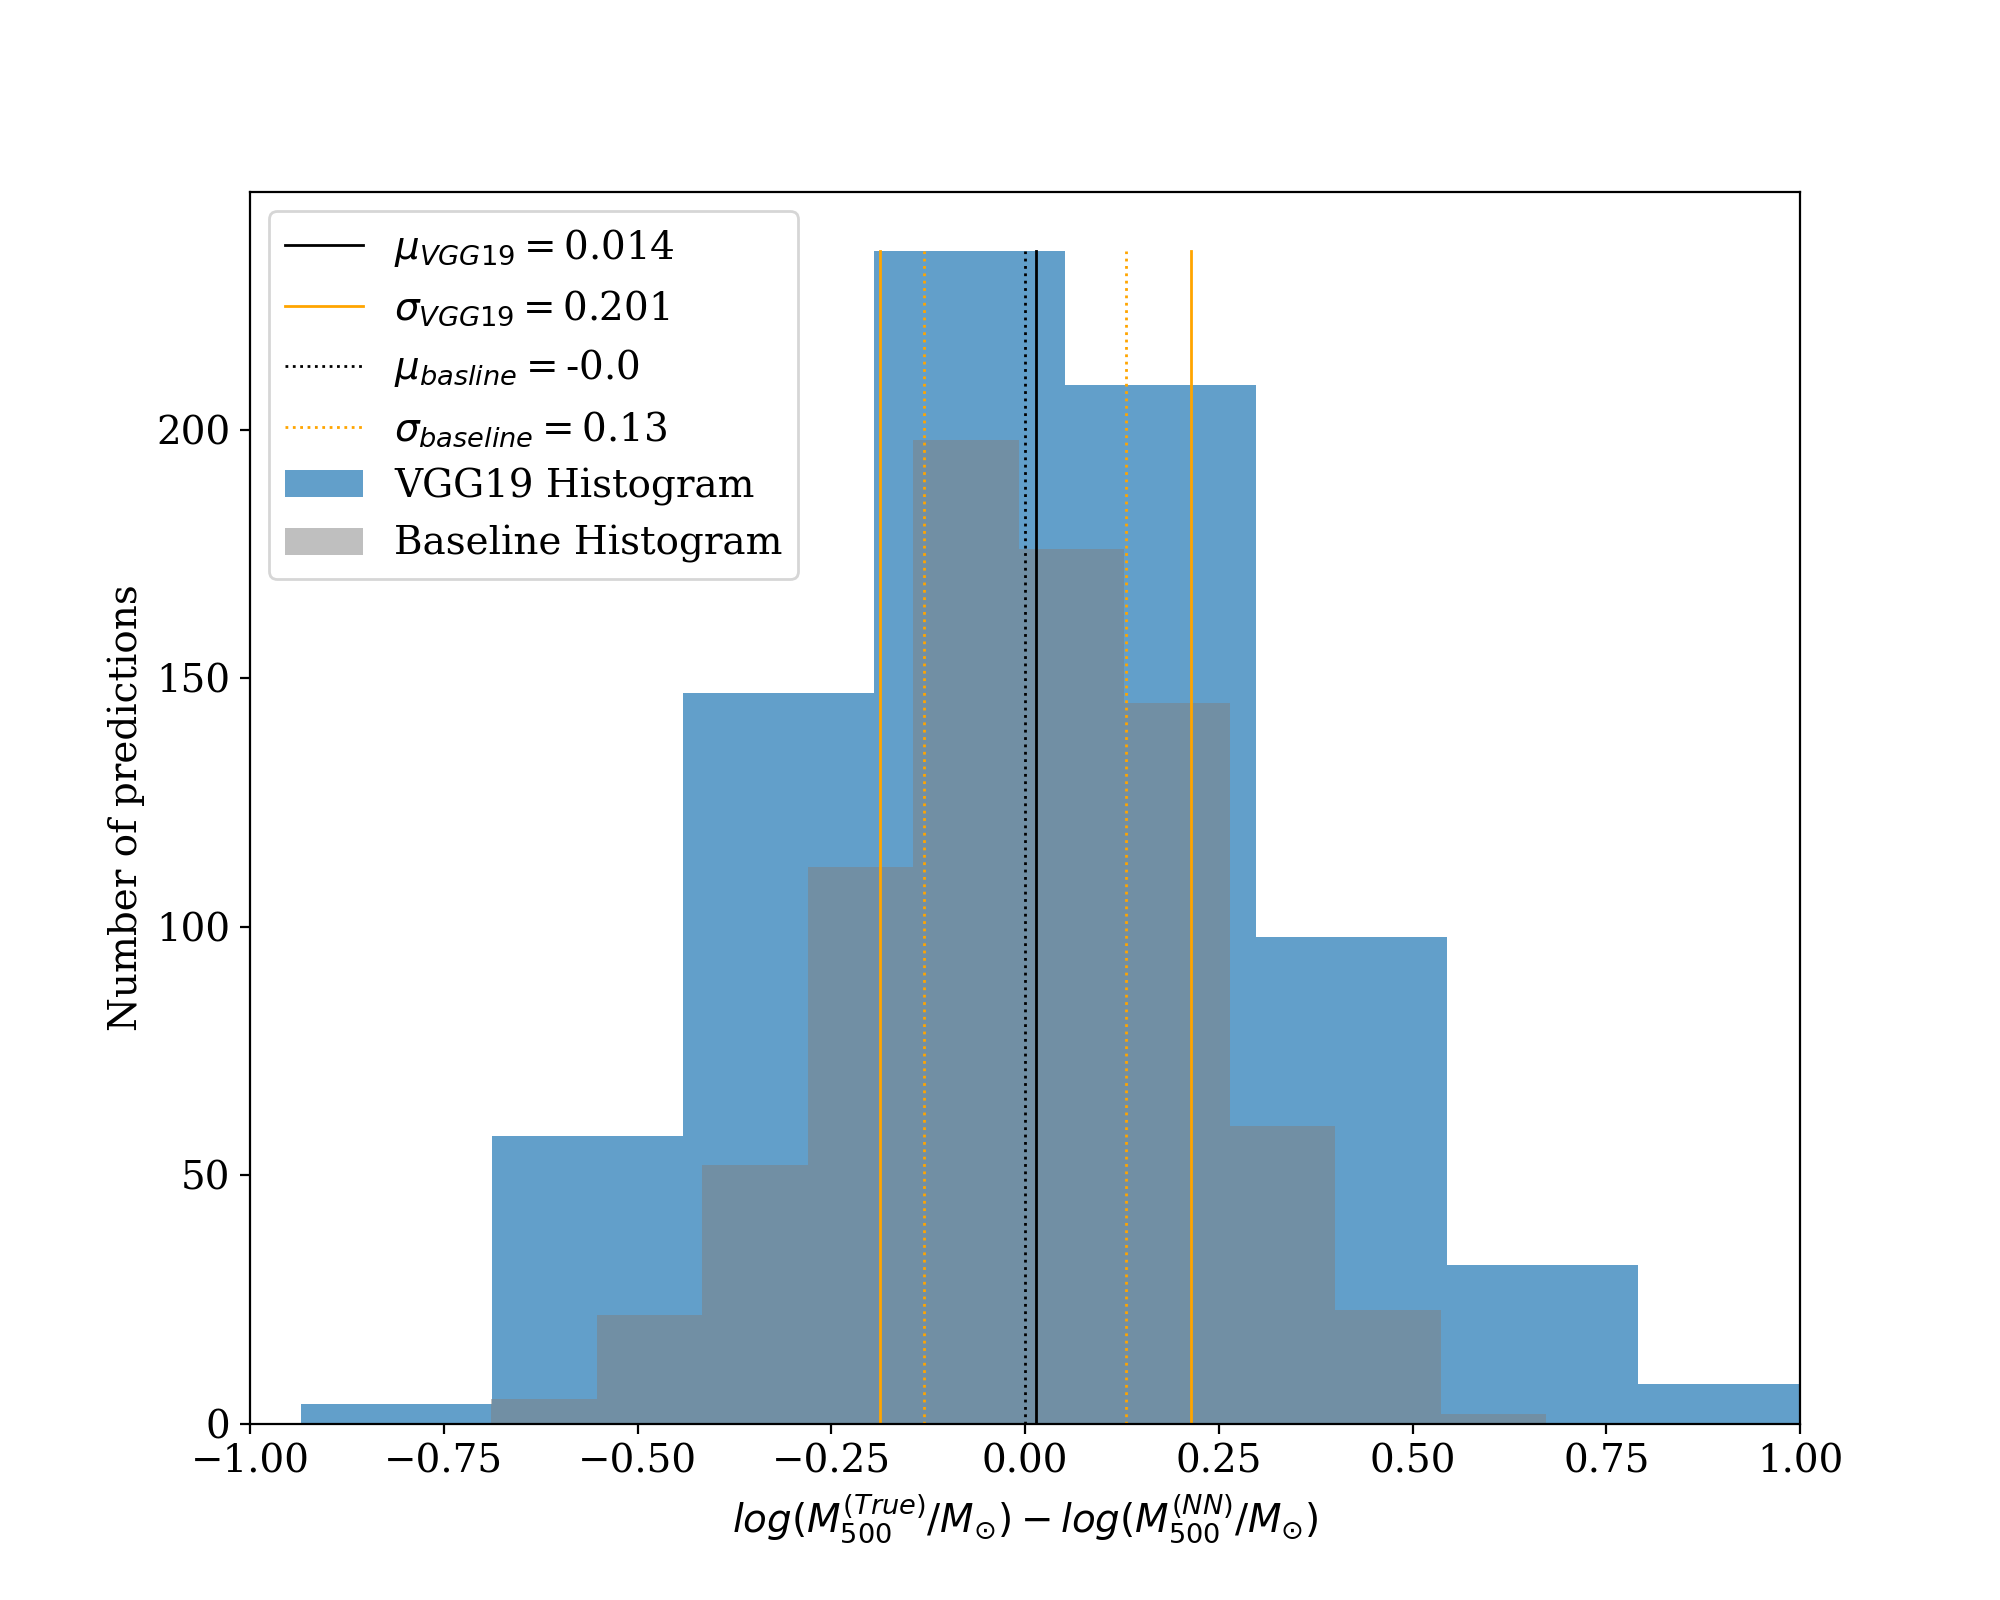
\includegraphics[width=\linewidth]{images/Chapter4/Results/test_VGG19_hist.png}
    \label{fig:test_VGG19_hist}
    \caption{VGG19}
\end{subfigure}
\begin{subfigure}{.325\textwidth}
    \centering
    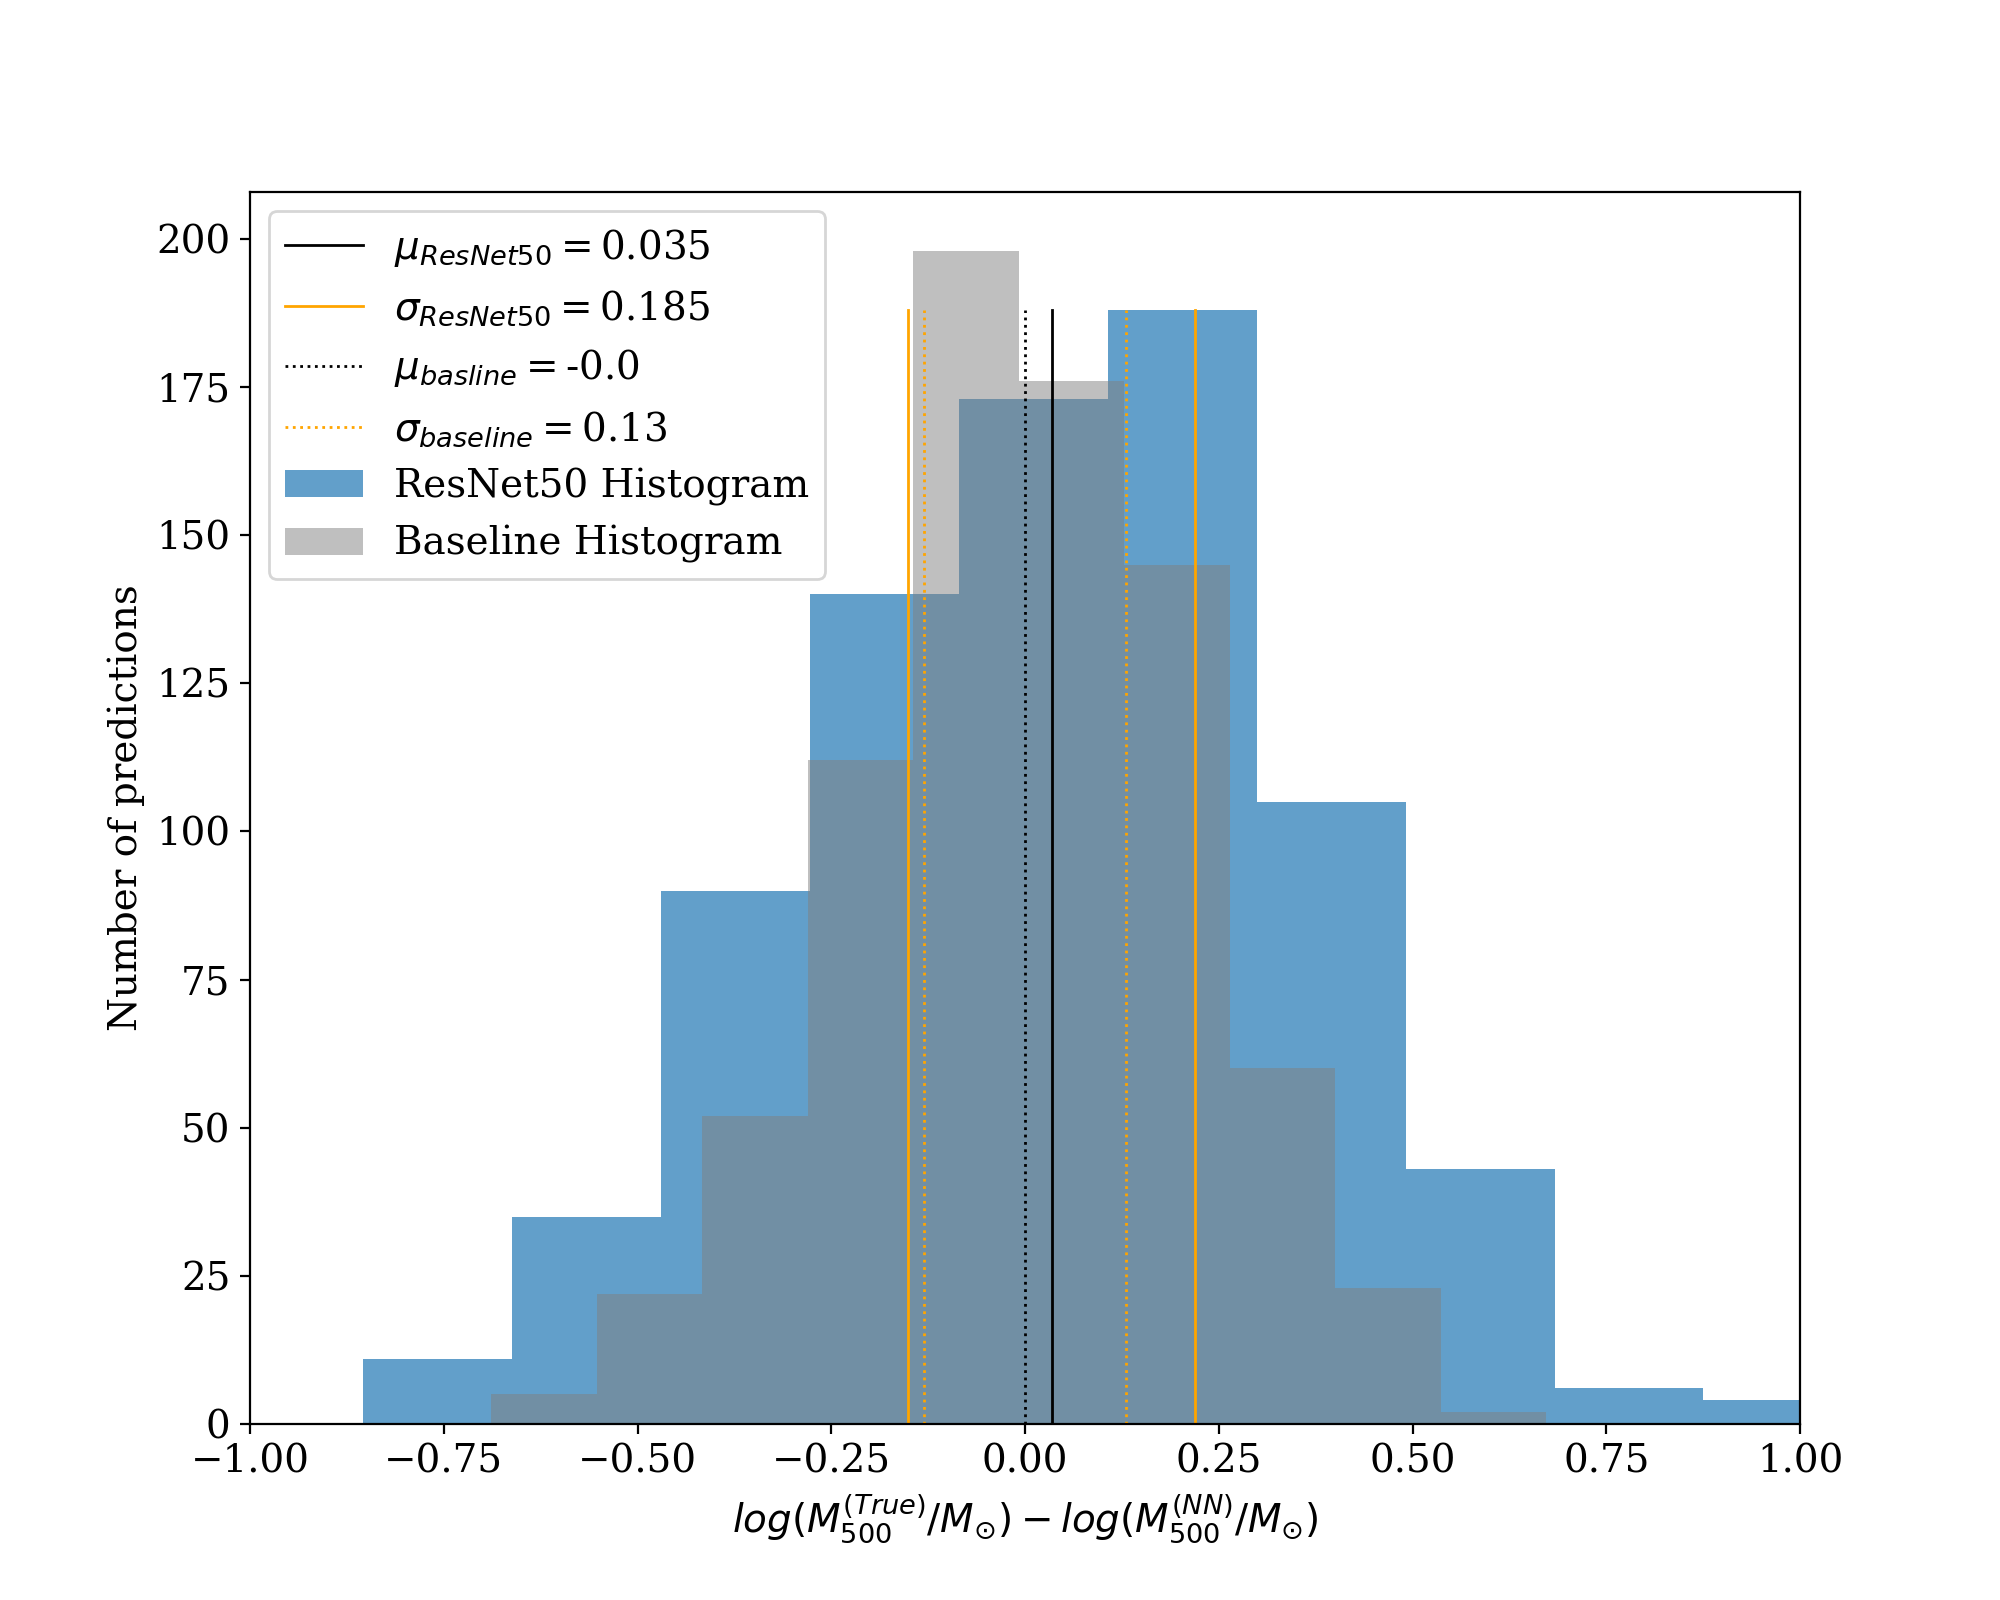
\includegraphics[width=\linewidth]{images/Chapter4/Results/test_ResNet50_hist.png}
    \label{fig:test_ResNet50_hist}
    \caption{ResNet50}
\end{subfigure}
\begin{subfigure}{.325\textwidth}
    \centering
    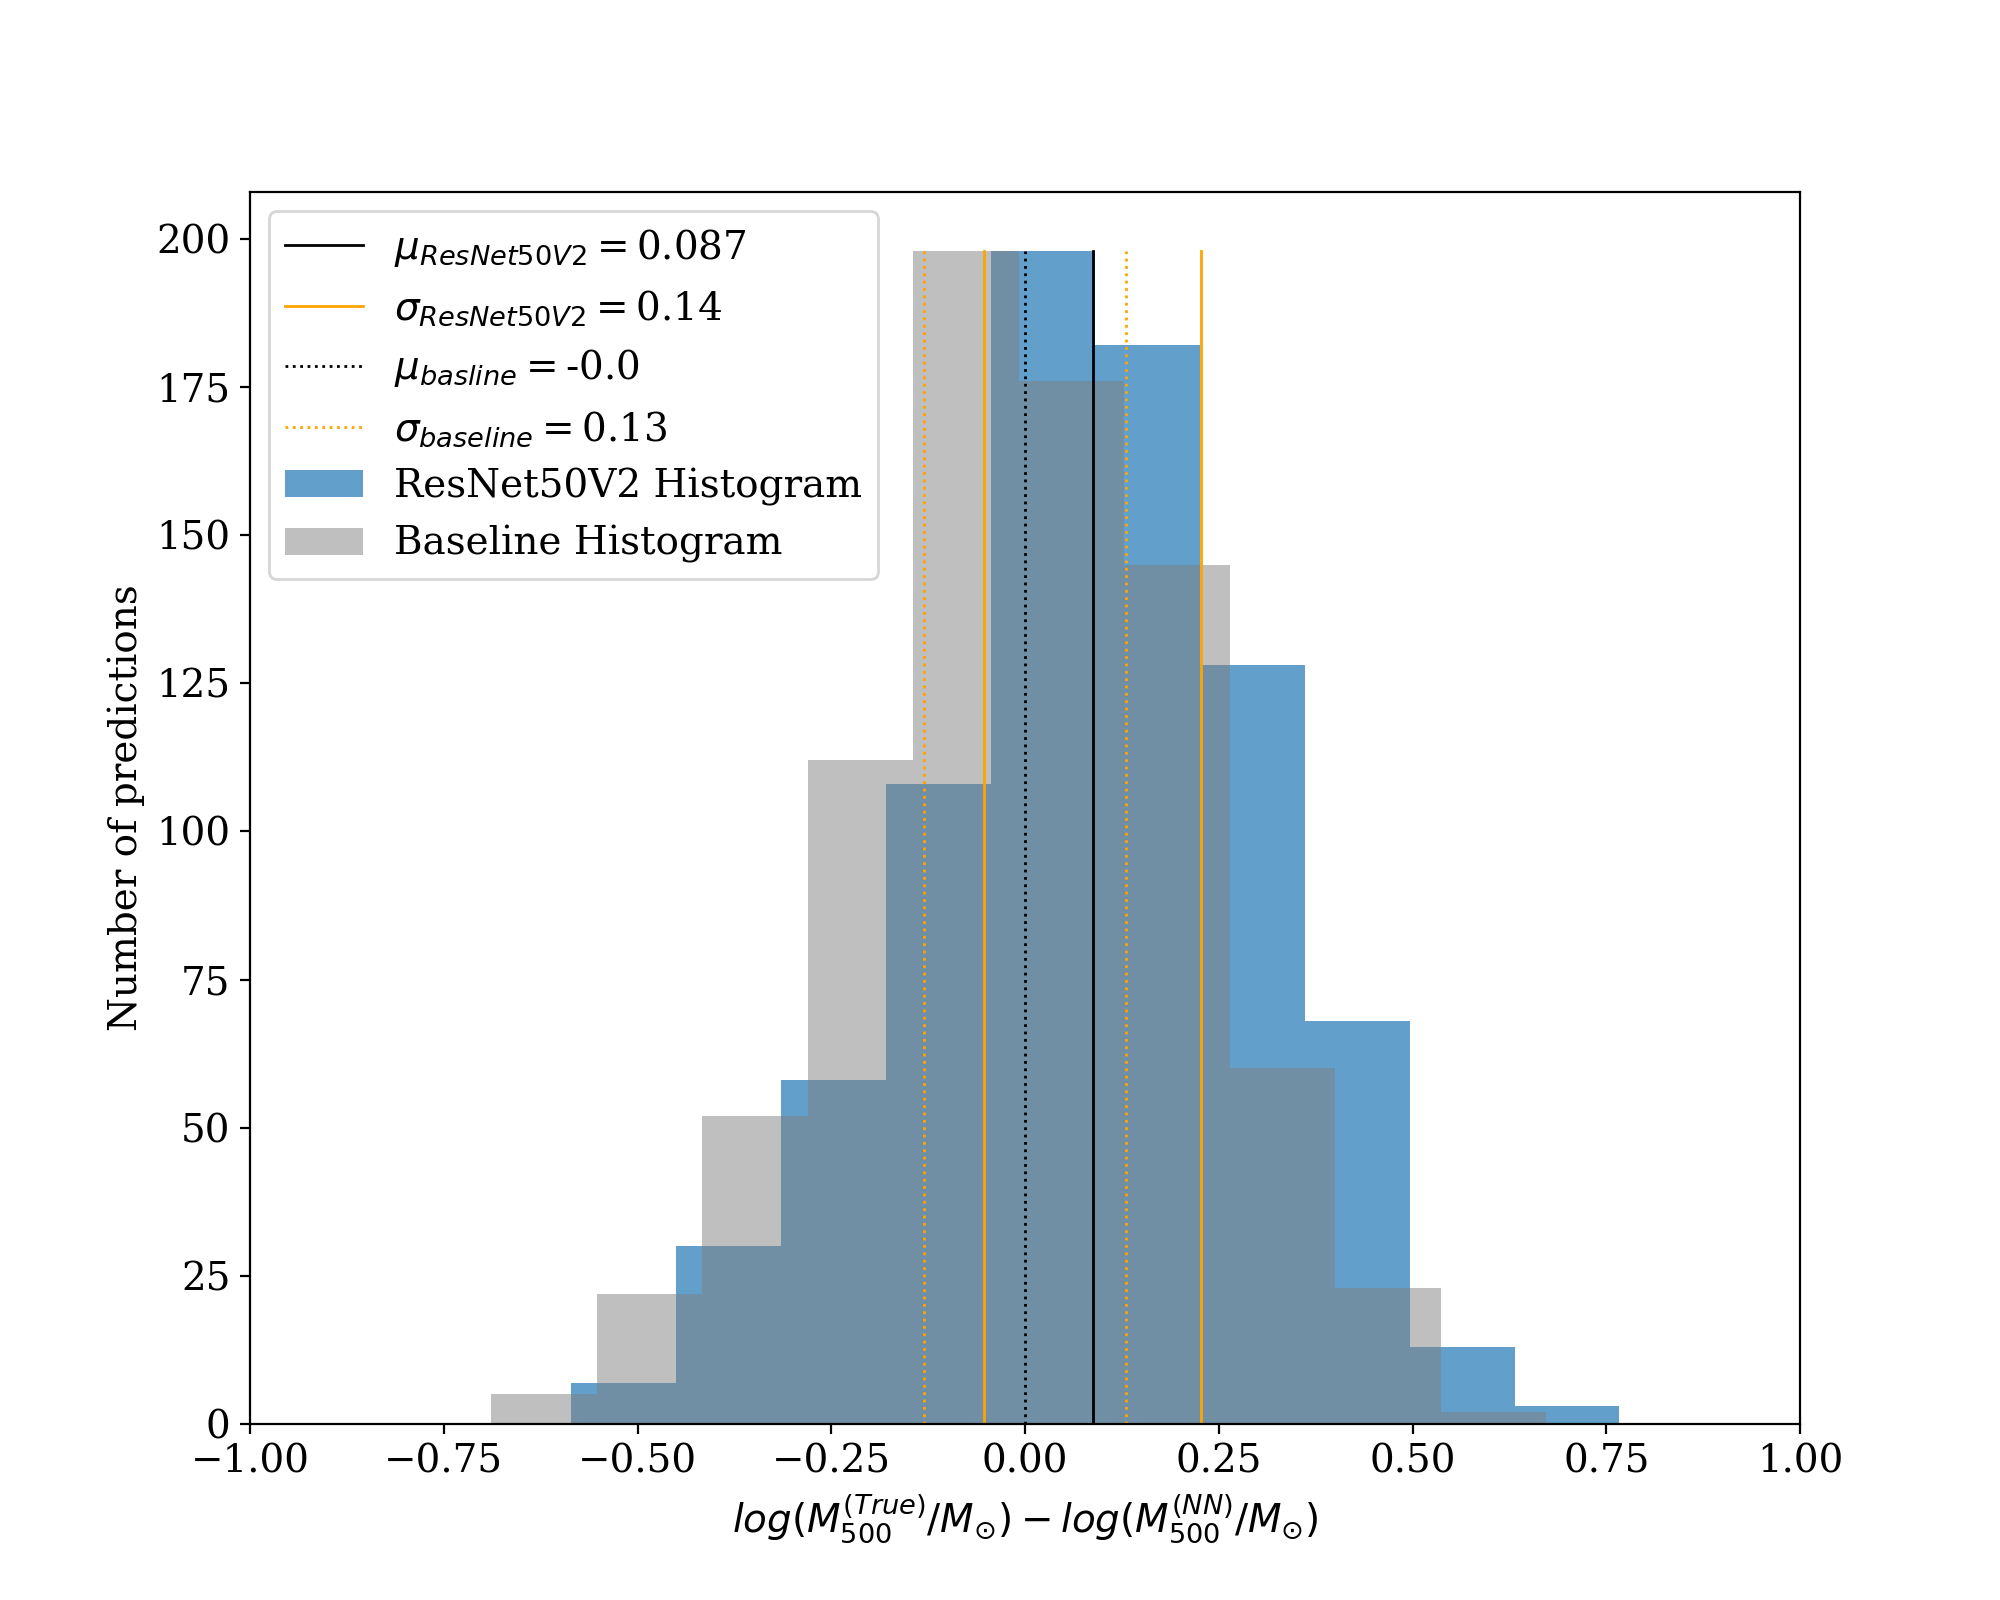
\includegraphics[width=\linewidth]{images/Chapter4/Results/test_ResNet50V2_hist.png}
    \label{fig:test_ResNet50V2_hist}
    \caption{ResNet50V2}
\end{subfigure}
\begin{subfigure}{.325\textwidth}
    \centering
    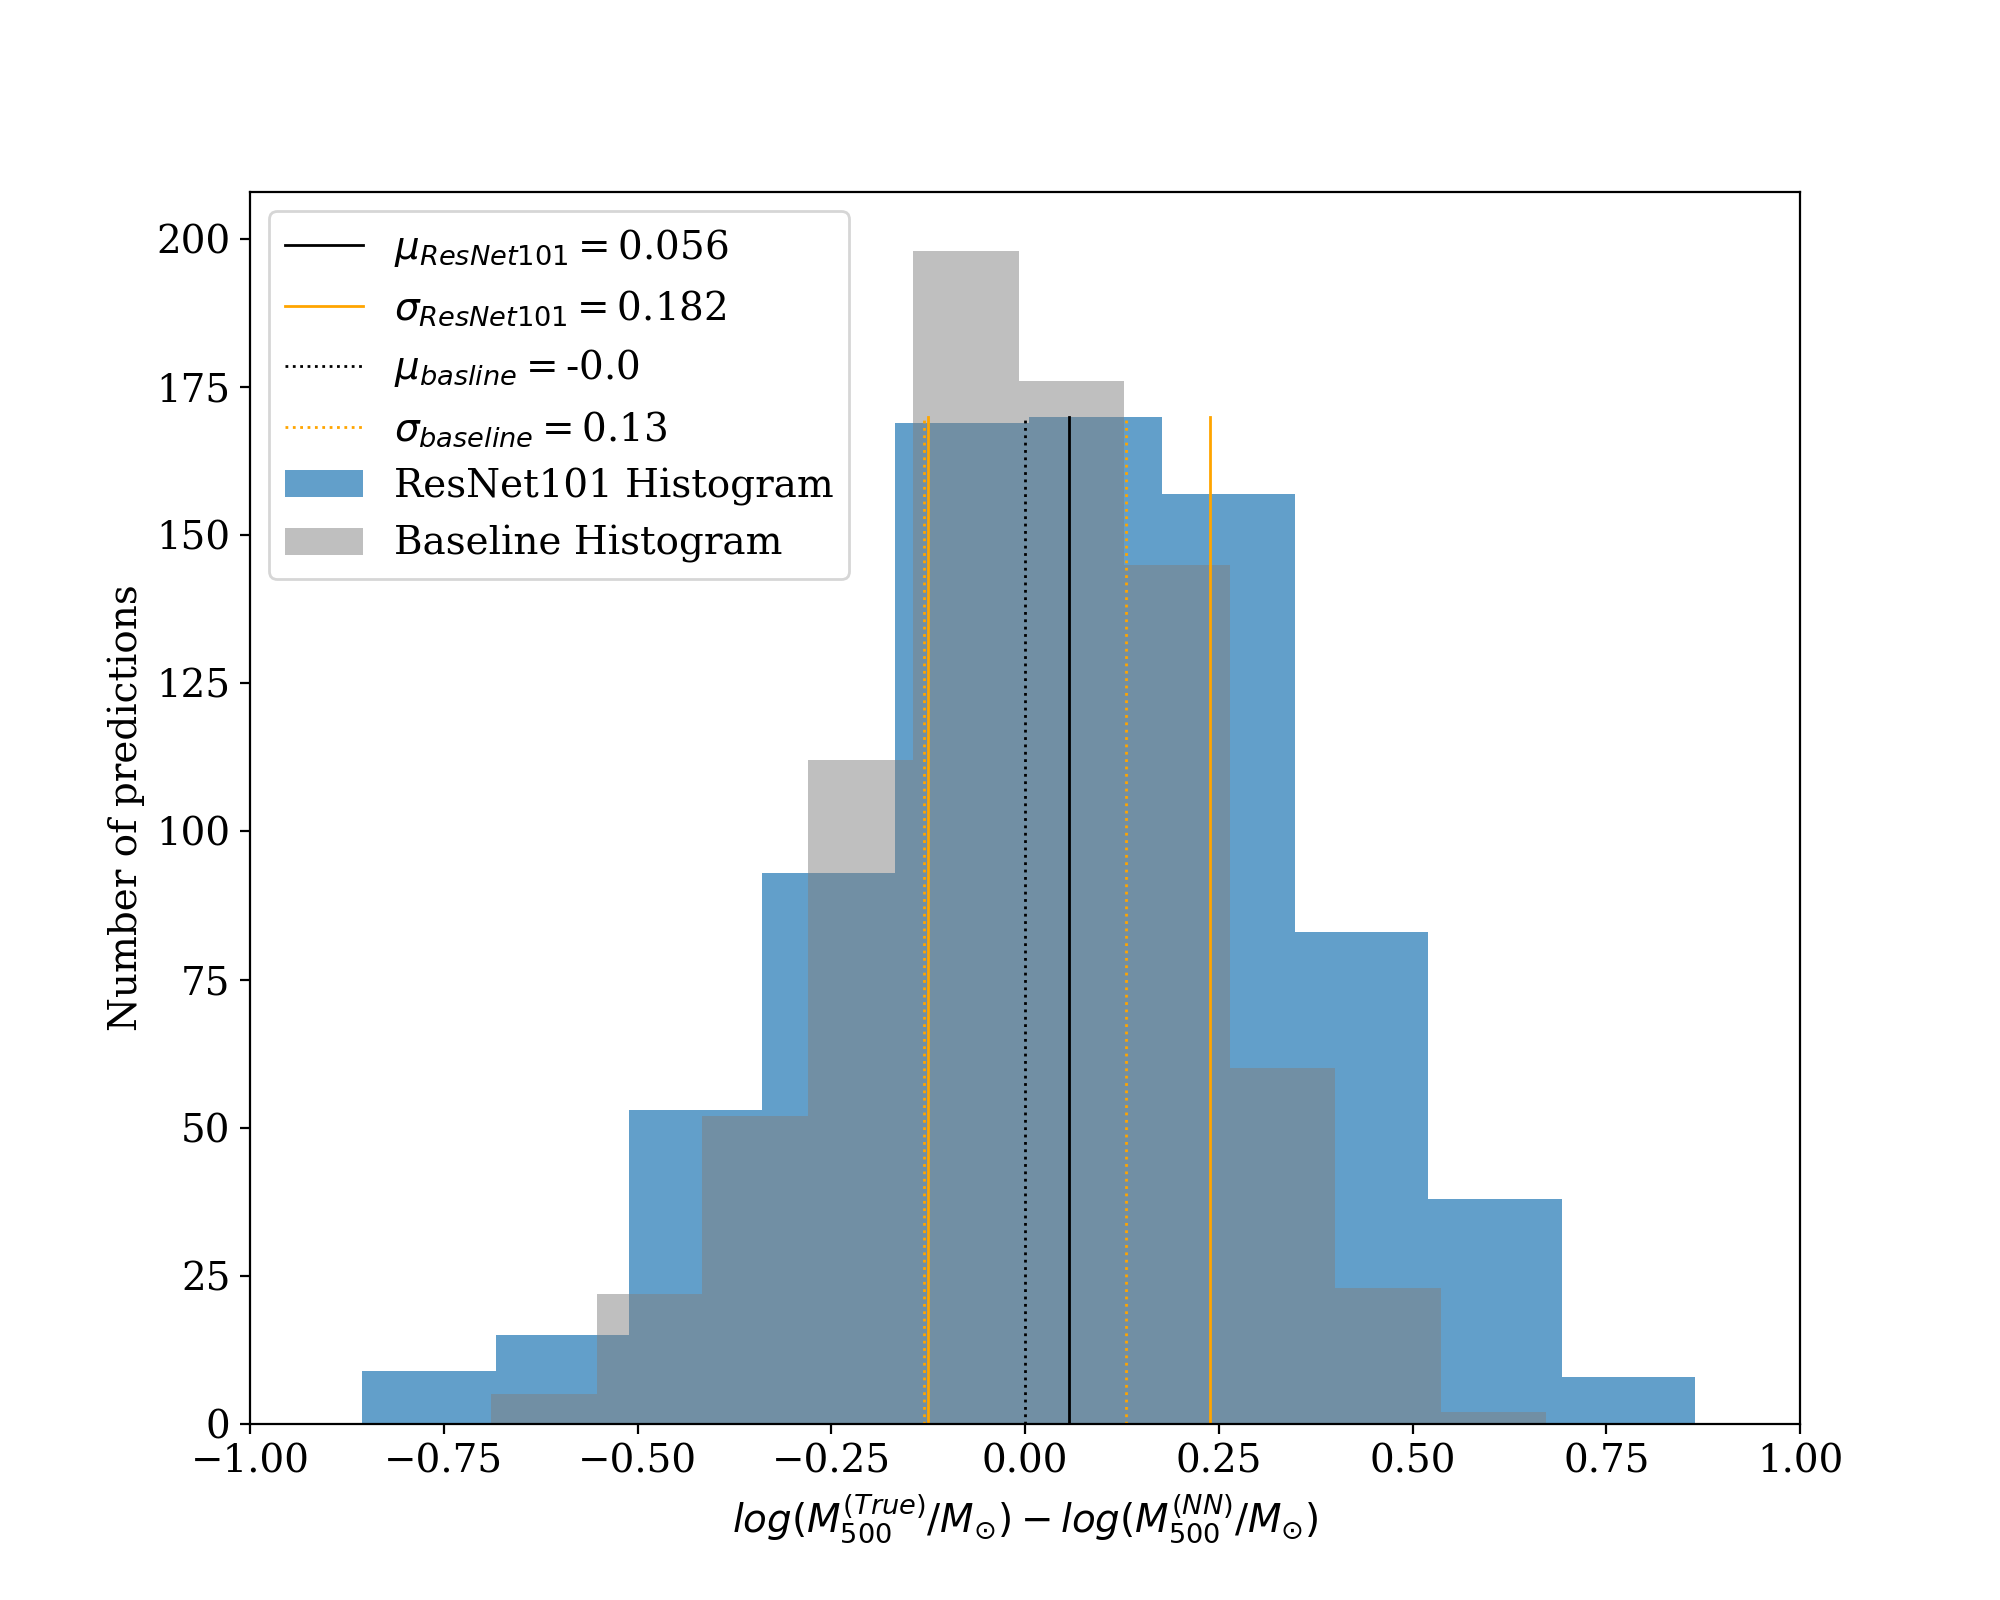
\includegraphics[width=\linewidth]{images/Chapter4/Results/test_ResNet101_hist.png}
    \label{fig:test_ResNet101_hist}
    \caption{ResNet101}
\end{subfigure}
\begin{subfigure}{.325\textwidth}
    \centering
    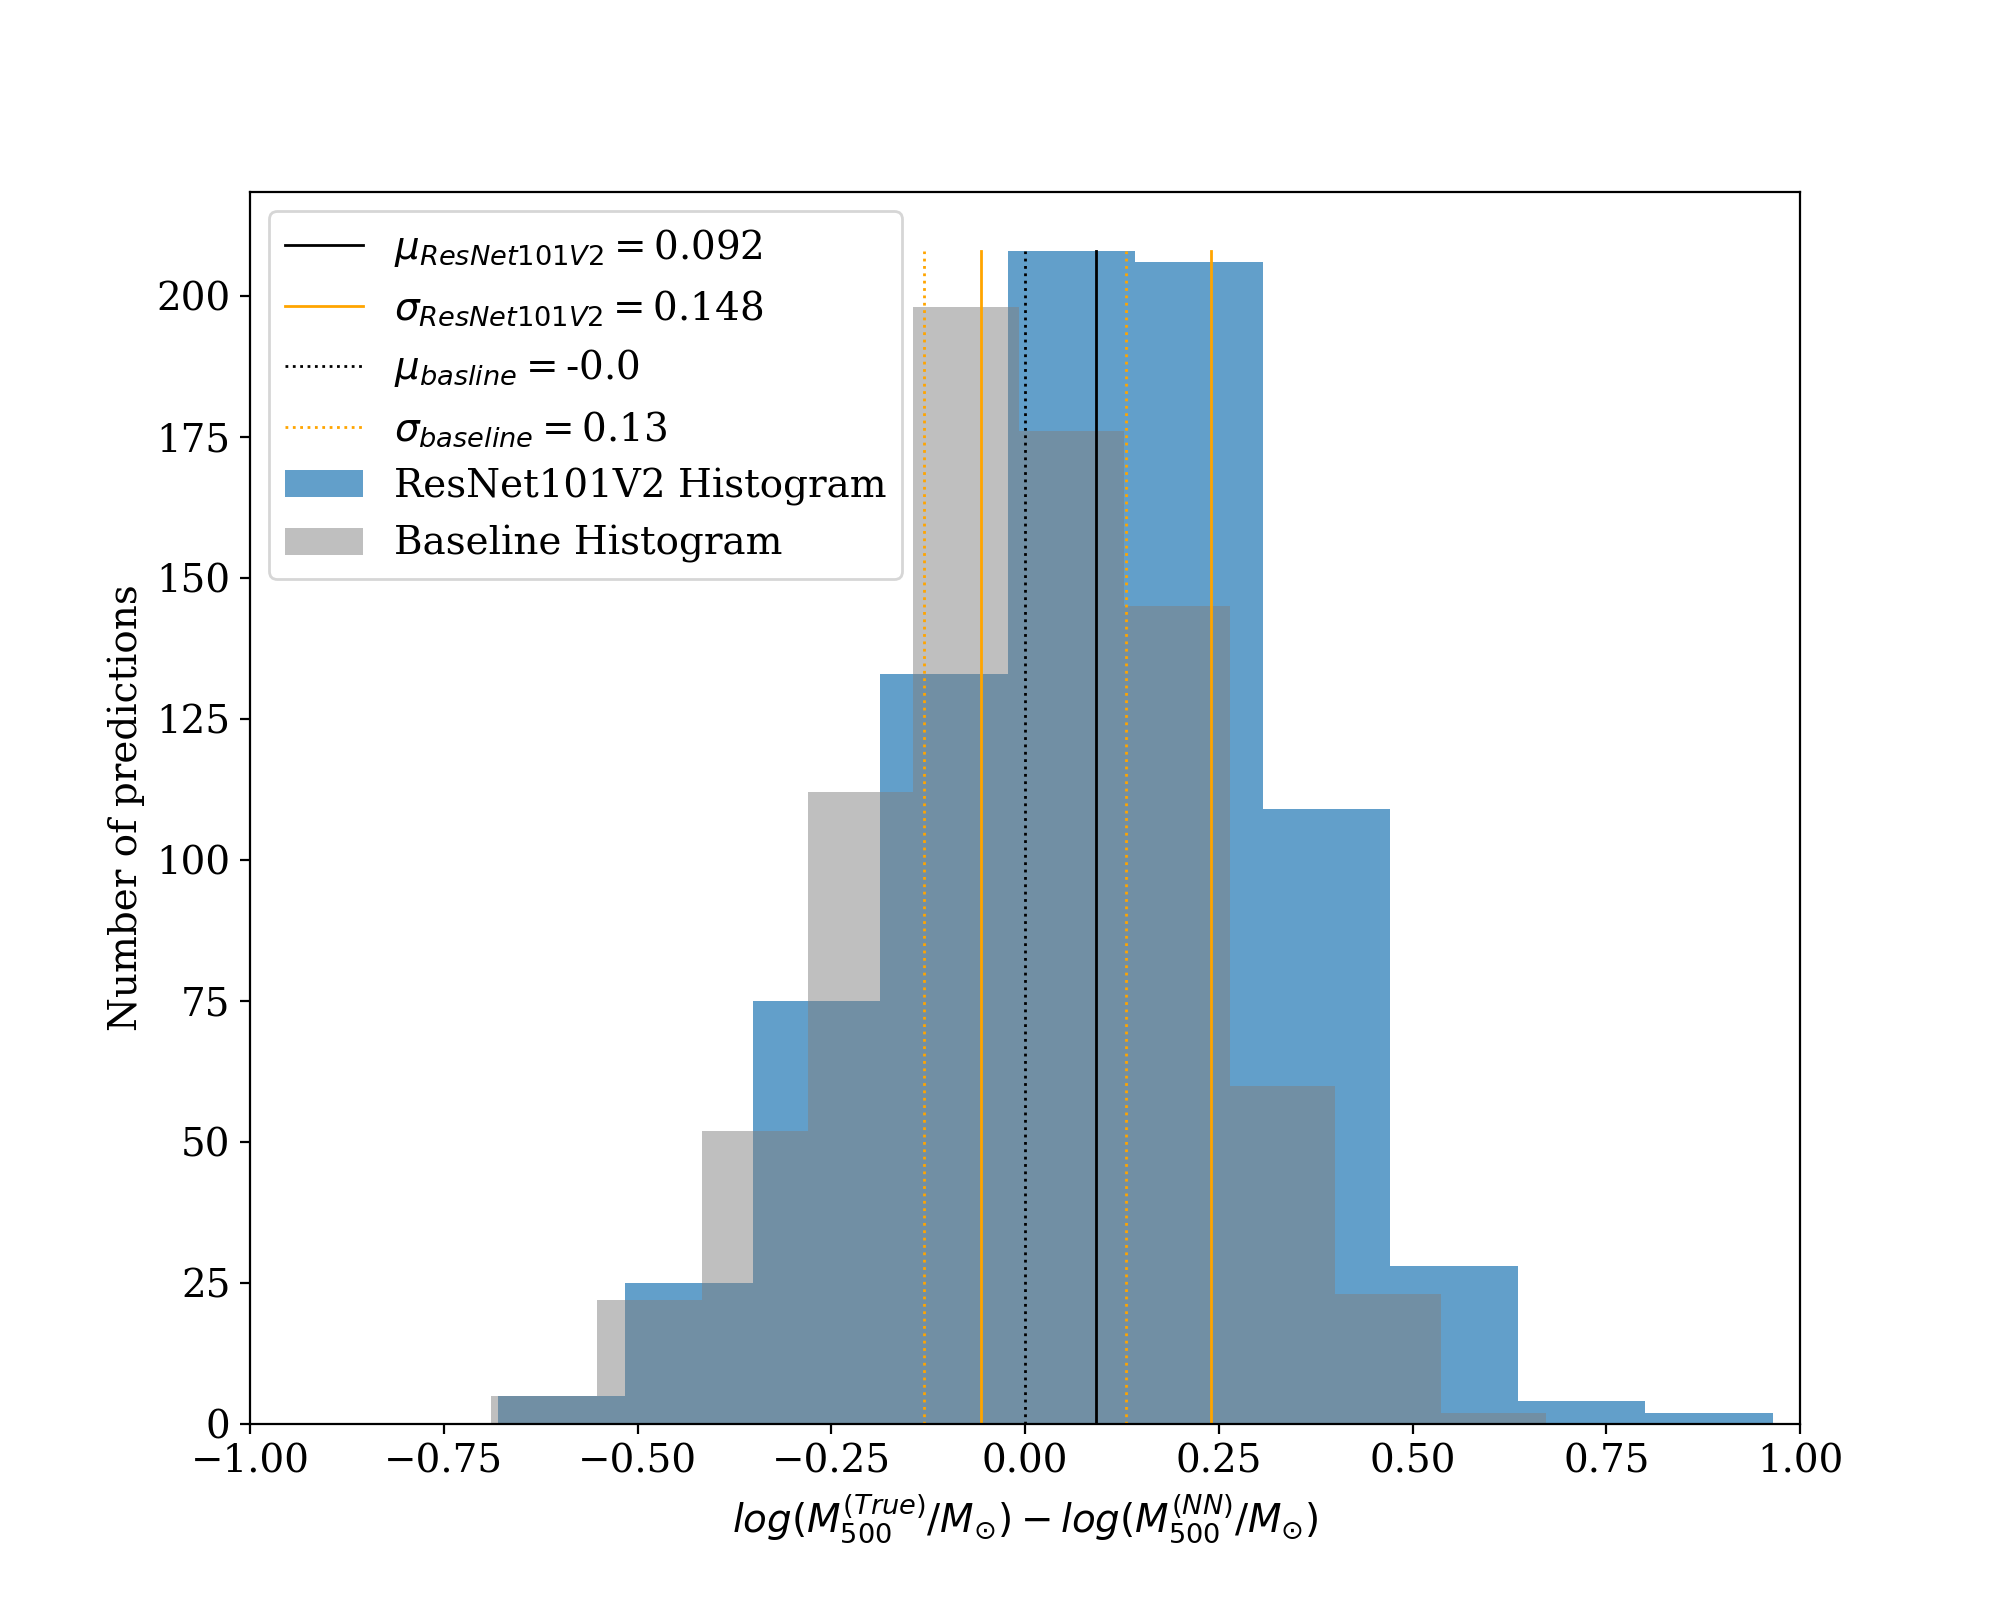
\includegraphics[width=\linewidth]{images/Chapter4/Results/test_ResNet101V2_hist.png}
    \label{fig:test_ResNet101V2_hist}
    \caption{ResNet101V2}
\end{subfigure}
\begin{subfigure}{.325\textwidth}
    \centering
    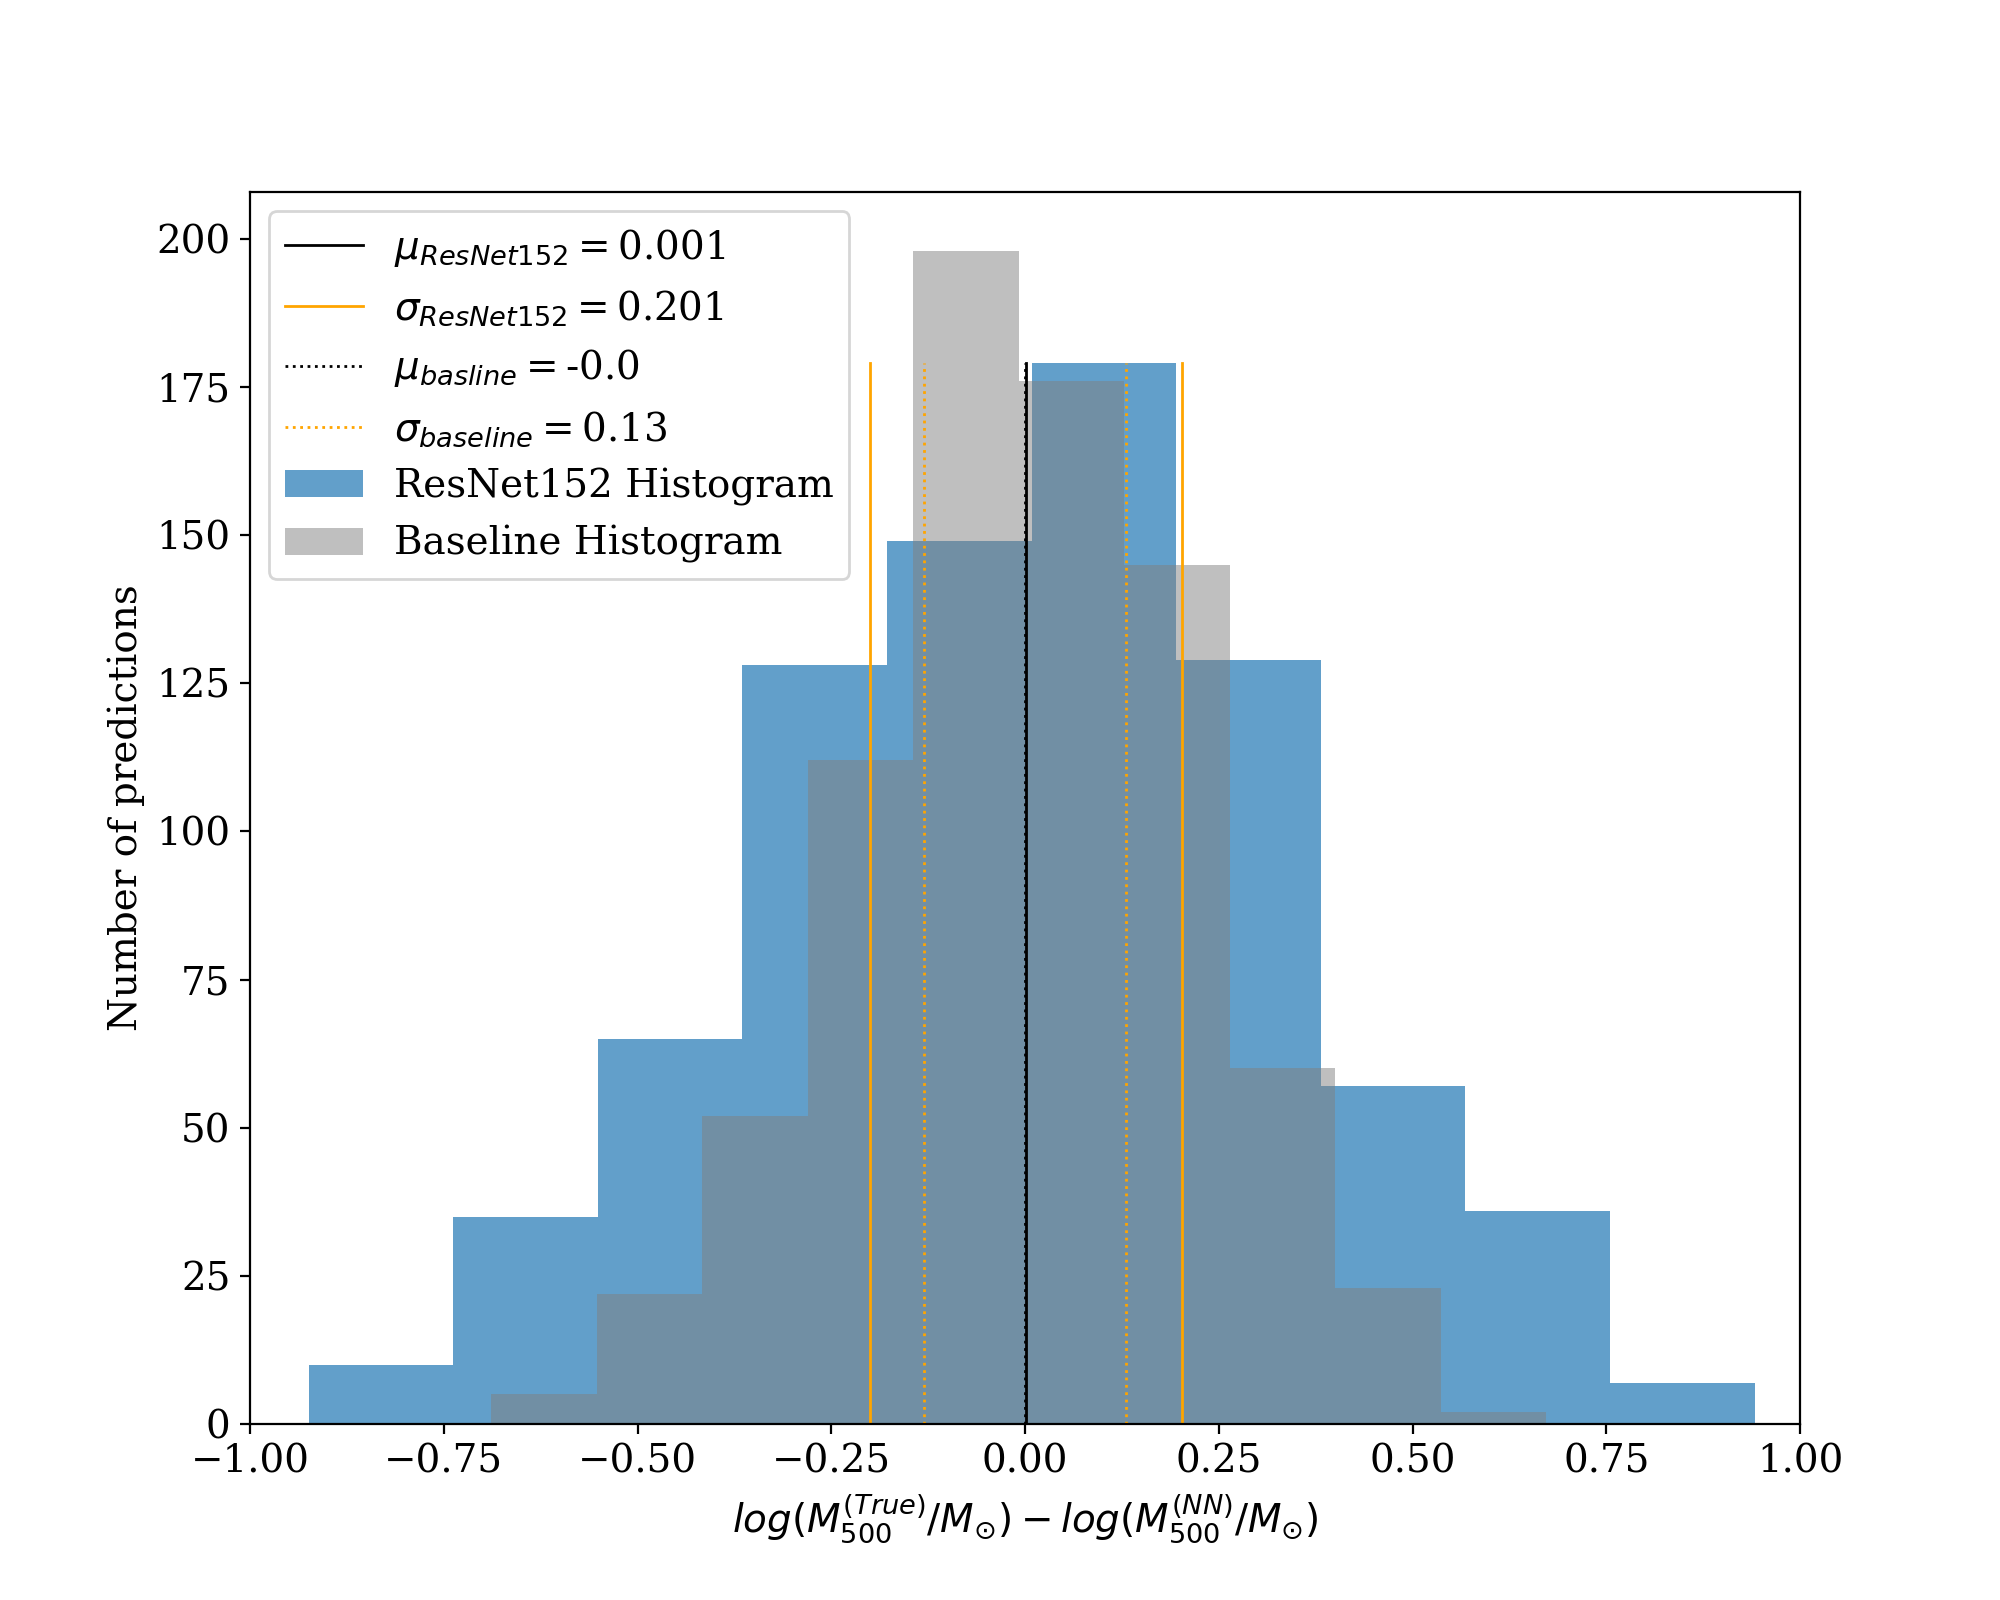
\includegraphics[width=\linewidth]{images/Chapter4/Results/test_ResNet152_hist.png}
    \label{fig:test_ResNet152_hist}
    \caption{ResNet152}
\end{subfigure}
\begin{subfigure}{.325\textwidth}
    \centering
    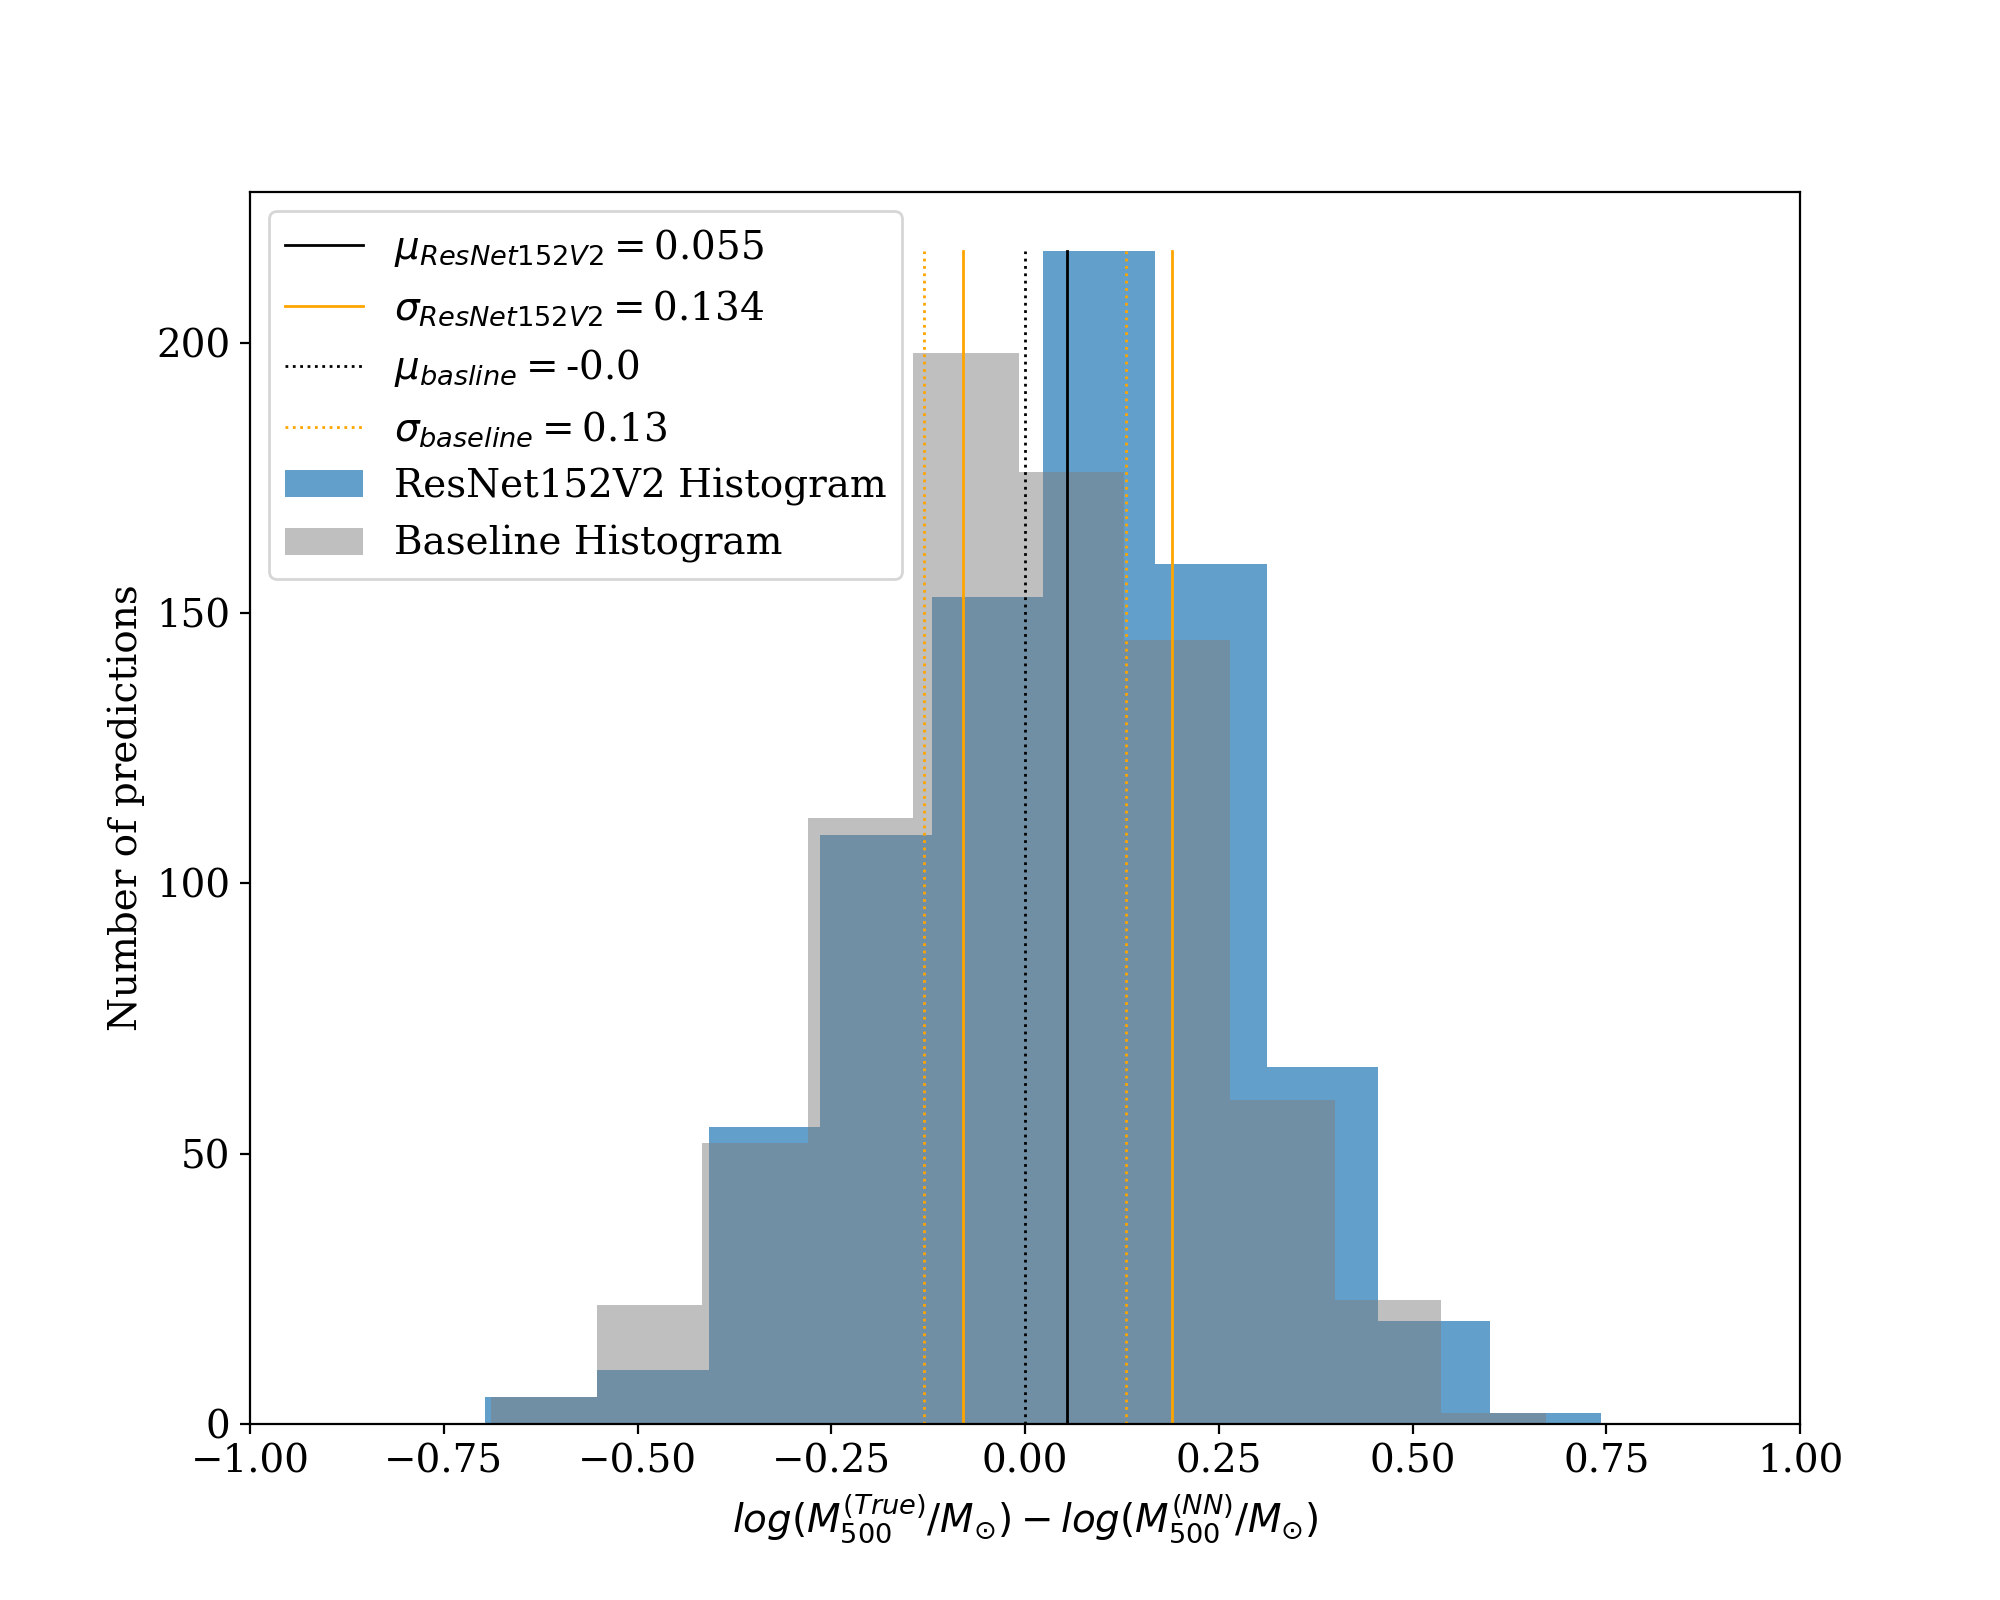
\includegraphics[width=\linewidth]{images/Chapter4/Results/test_ResNet152V2_hist.png}
    \label{fig:test_ResNet152V2_hist}
    \caption{ResNet152V2}
\end{subfigure}
\begin{subfigure}{.325\textwidth}
    \centering
    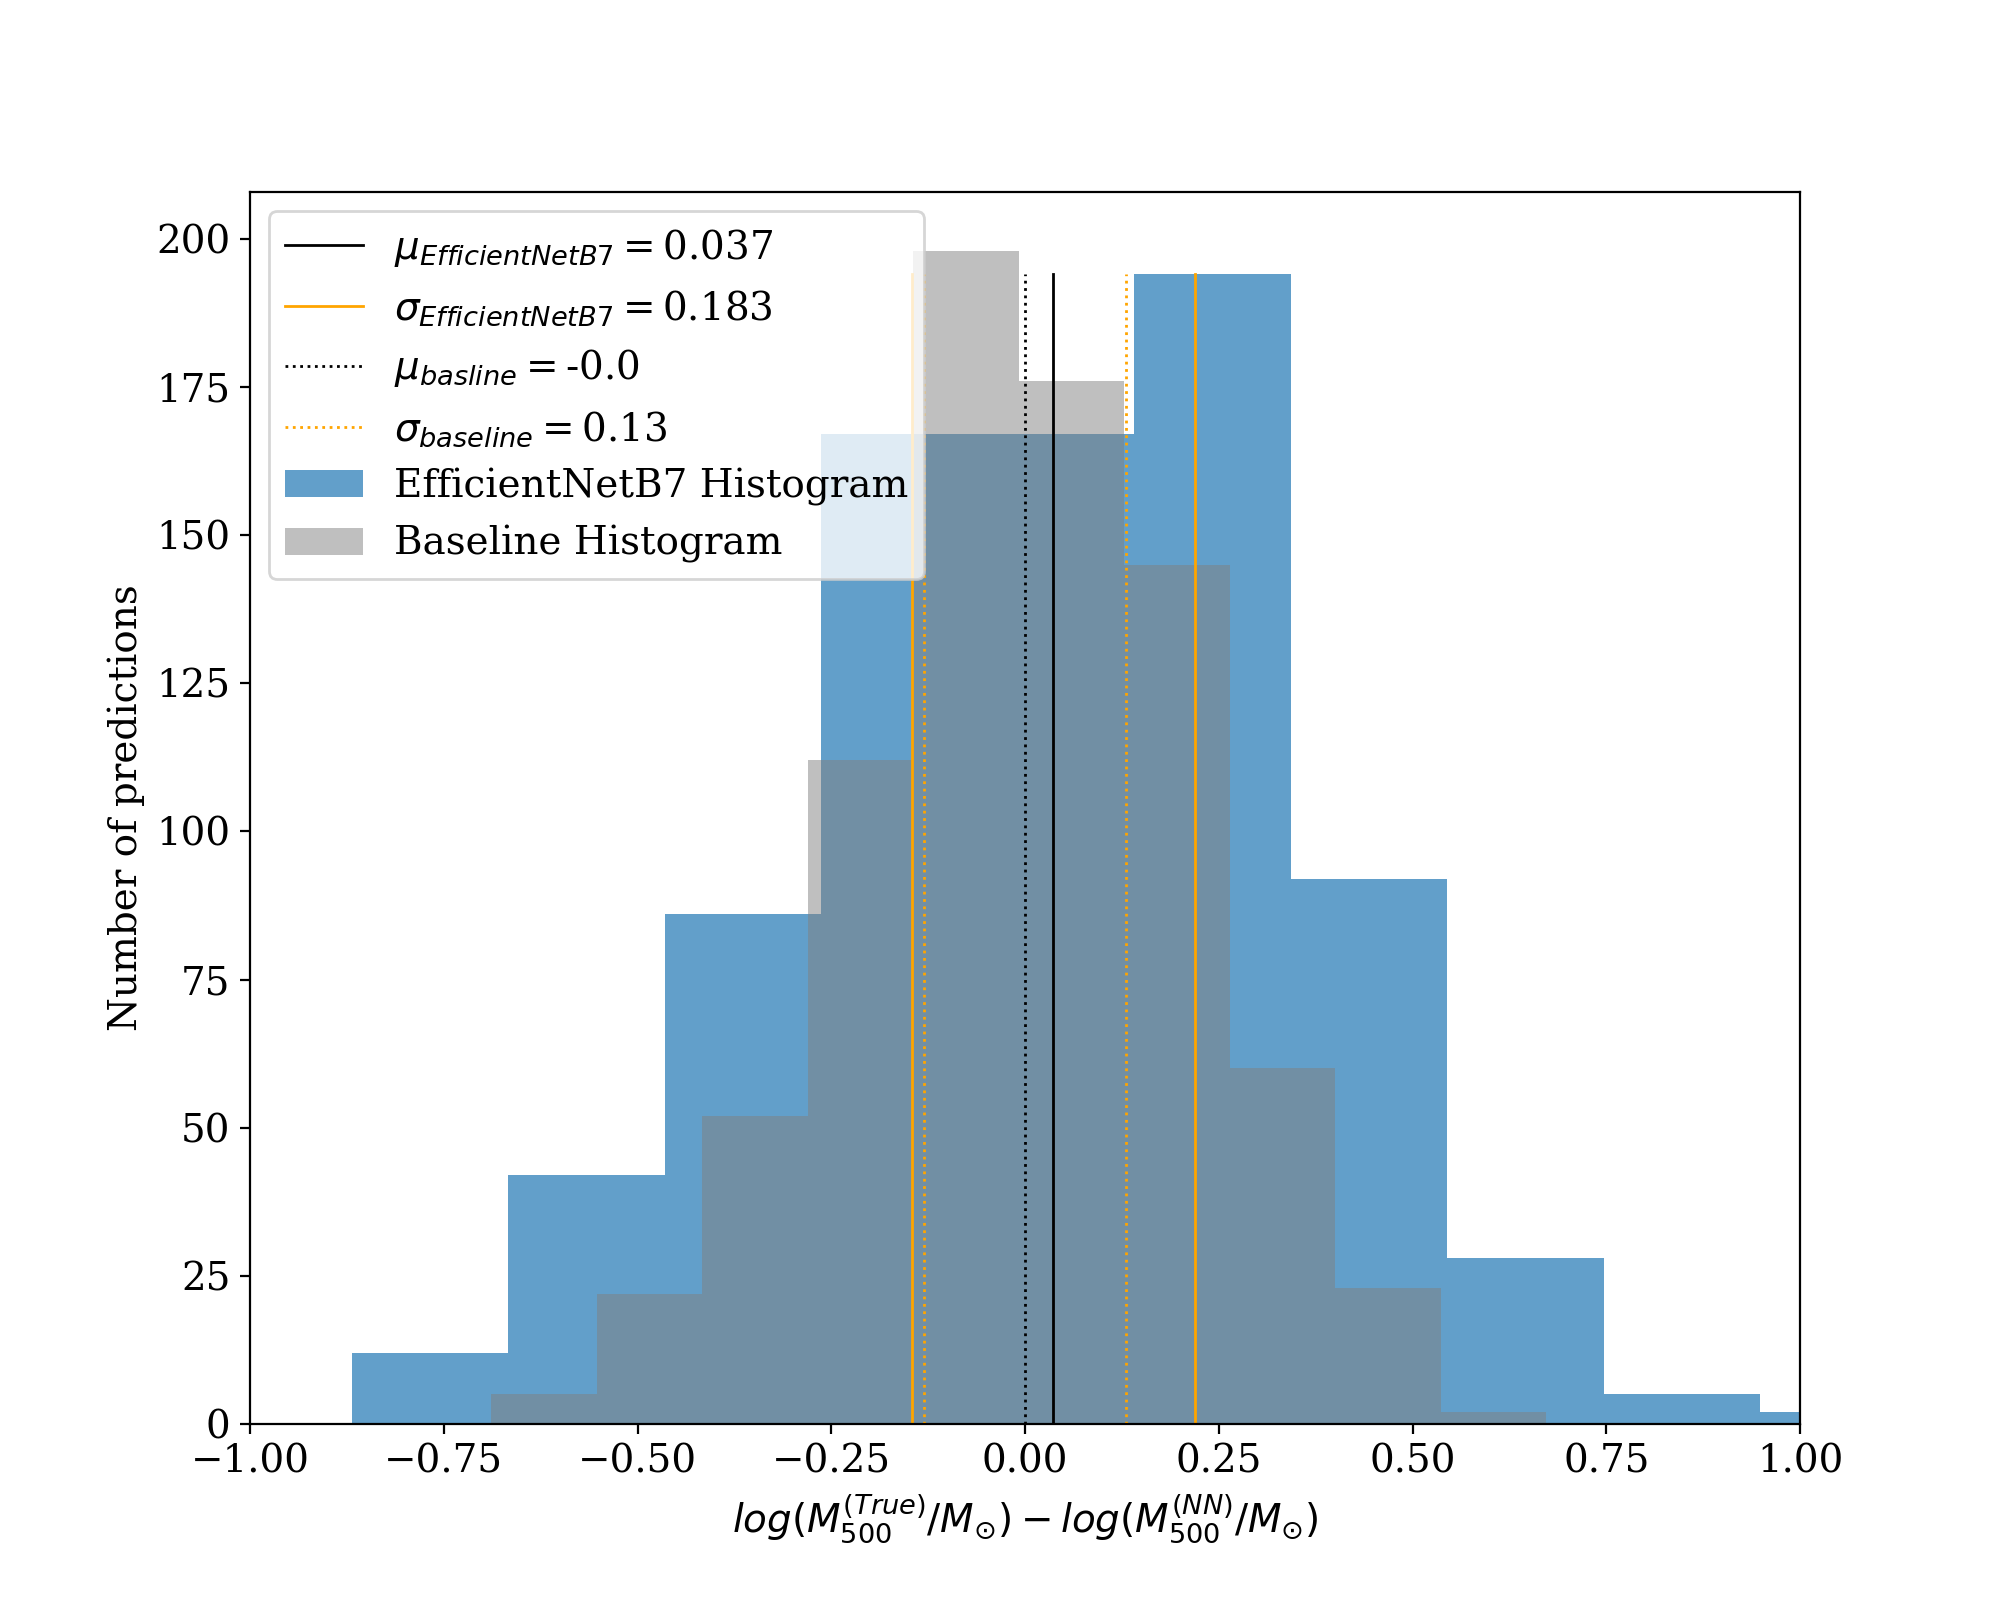
\includegraphics[width=\linewidth]{images/Chapter4/Results/test_EfficientNetB7_hist.png}
    \label{fig:test_EfficientNetB7_hist}
    \caption{EfficientNetB7}
\end{subfigure}
\caption{Comparison histograms between each deep model's best predictions (\textit{blue}) and the best predictions from the basic CNN (\textit{grey}) on the test set.}
\end{figure}





\begin{figure}[H]
\centering
\begin{subfigure}{.325\textwidth}
    \centering
    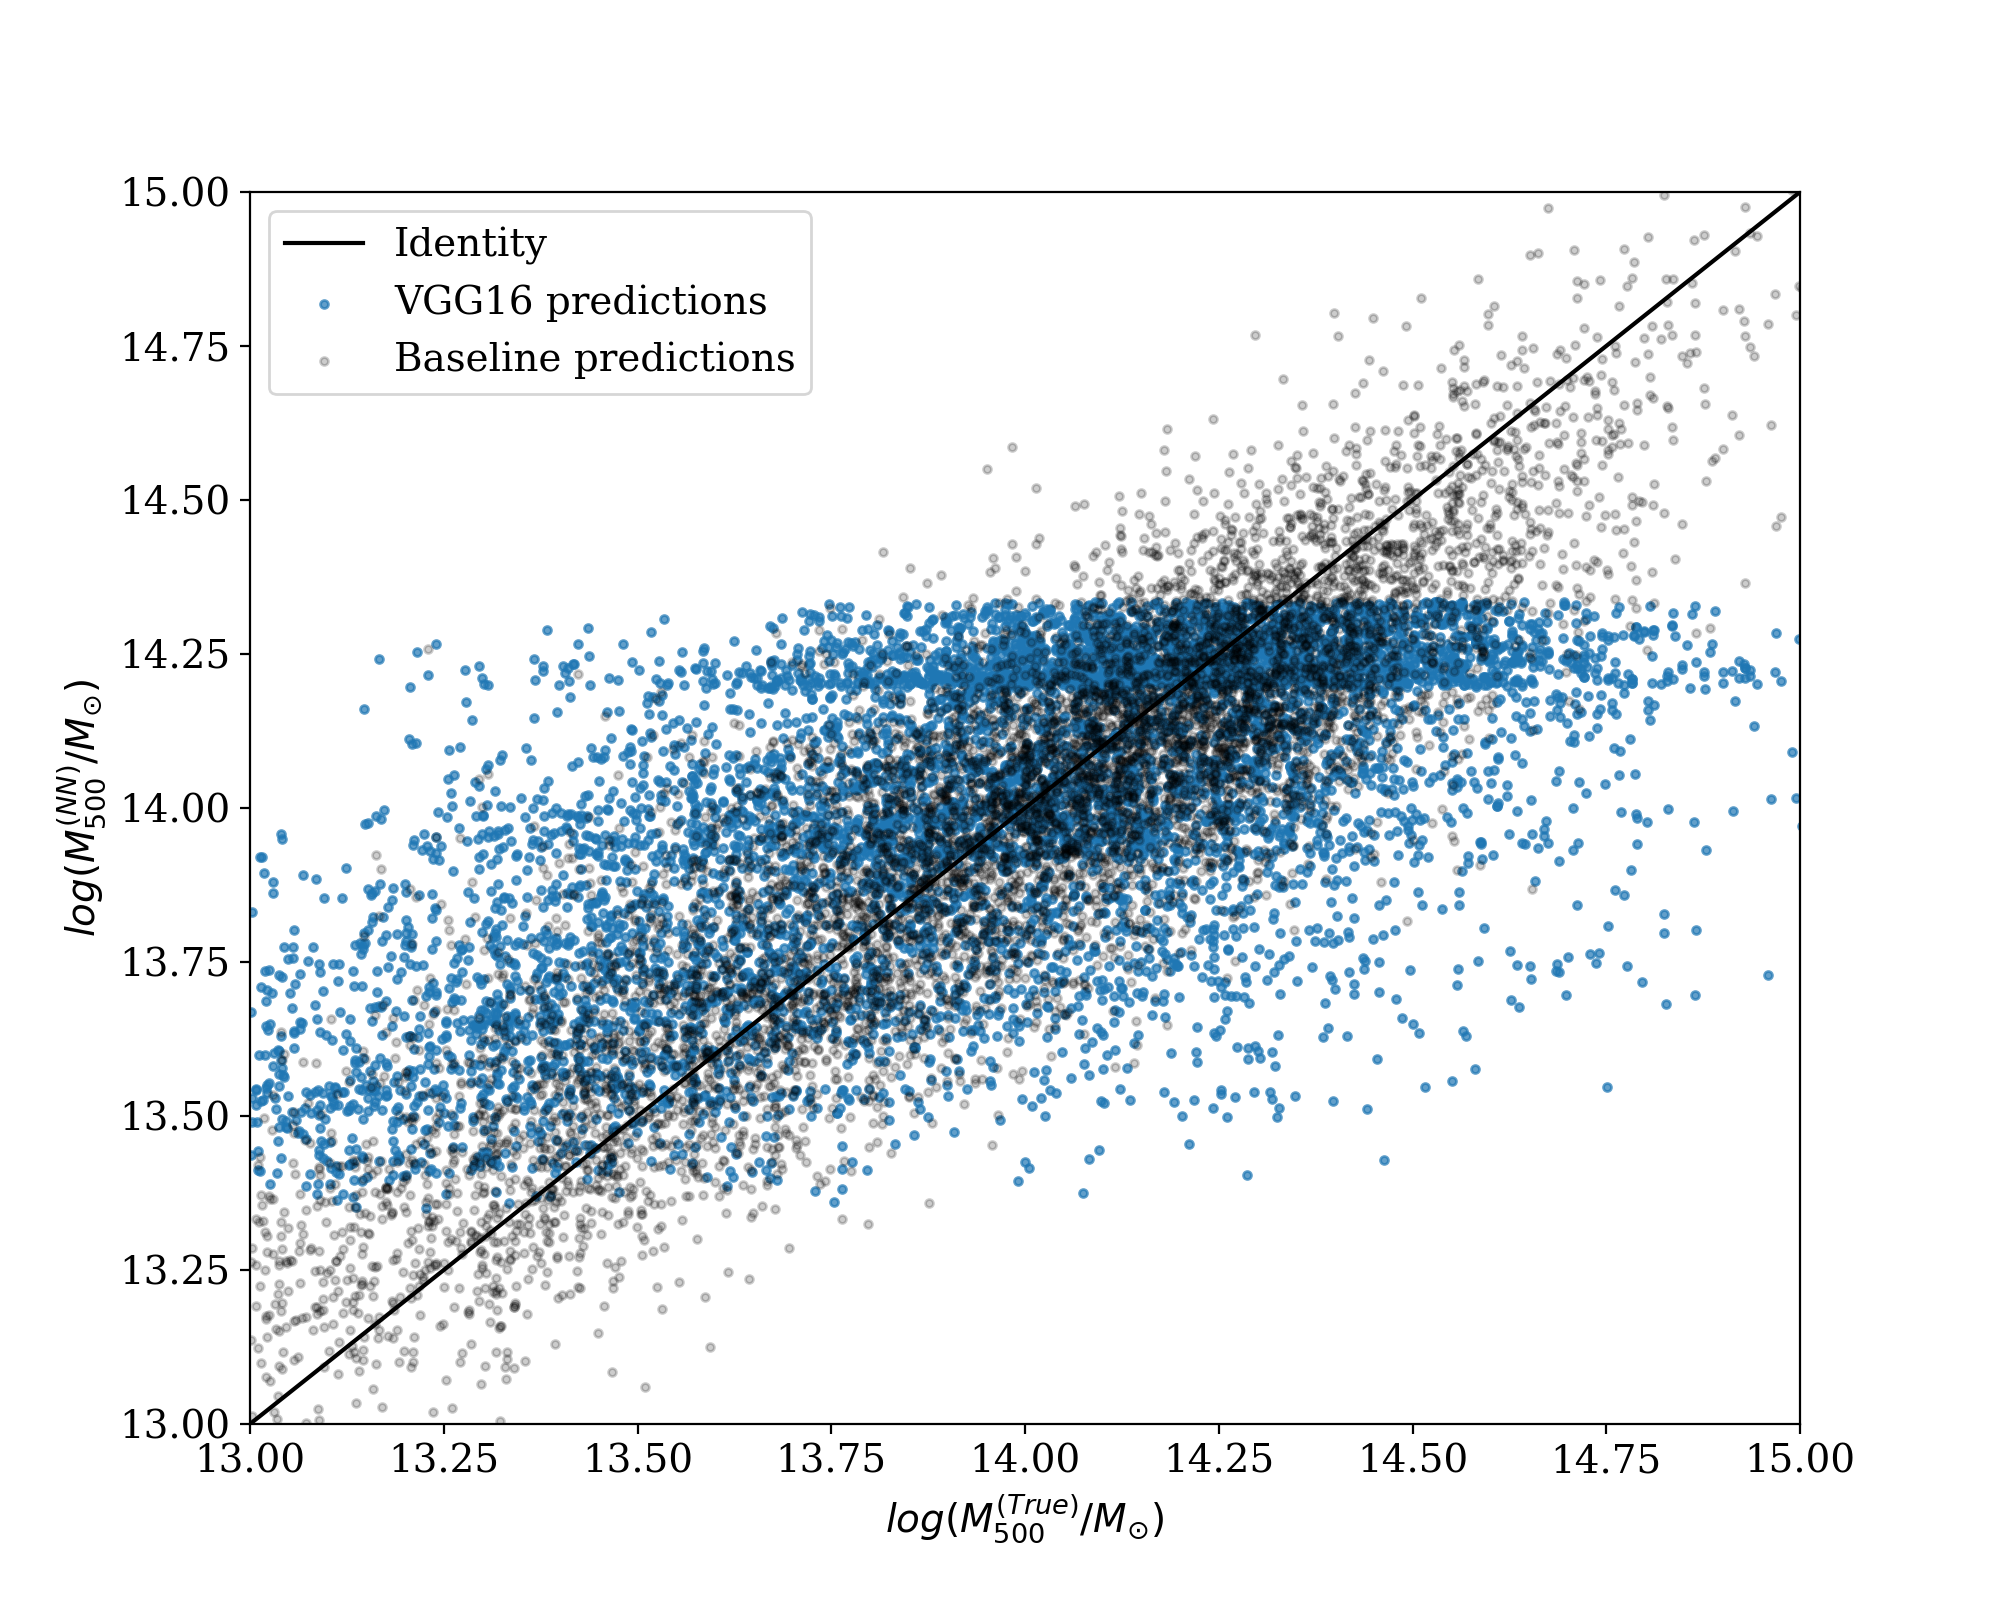
\includegraphics[width=\linewidth]{images/Chapter4/Results/training_VGG16_scatter.png}
    \label{fig:training_VGG16_scatter}
    \caption{VGG16}
\end{subfigure}
\begin{subfigure}{.325\textwidth}
    \centering
    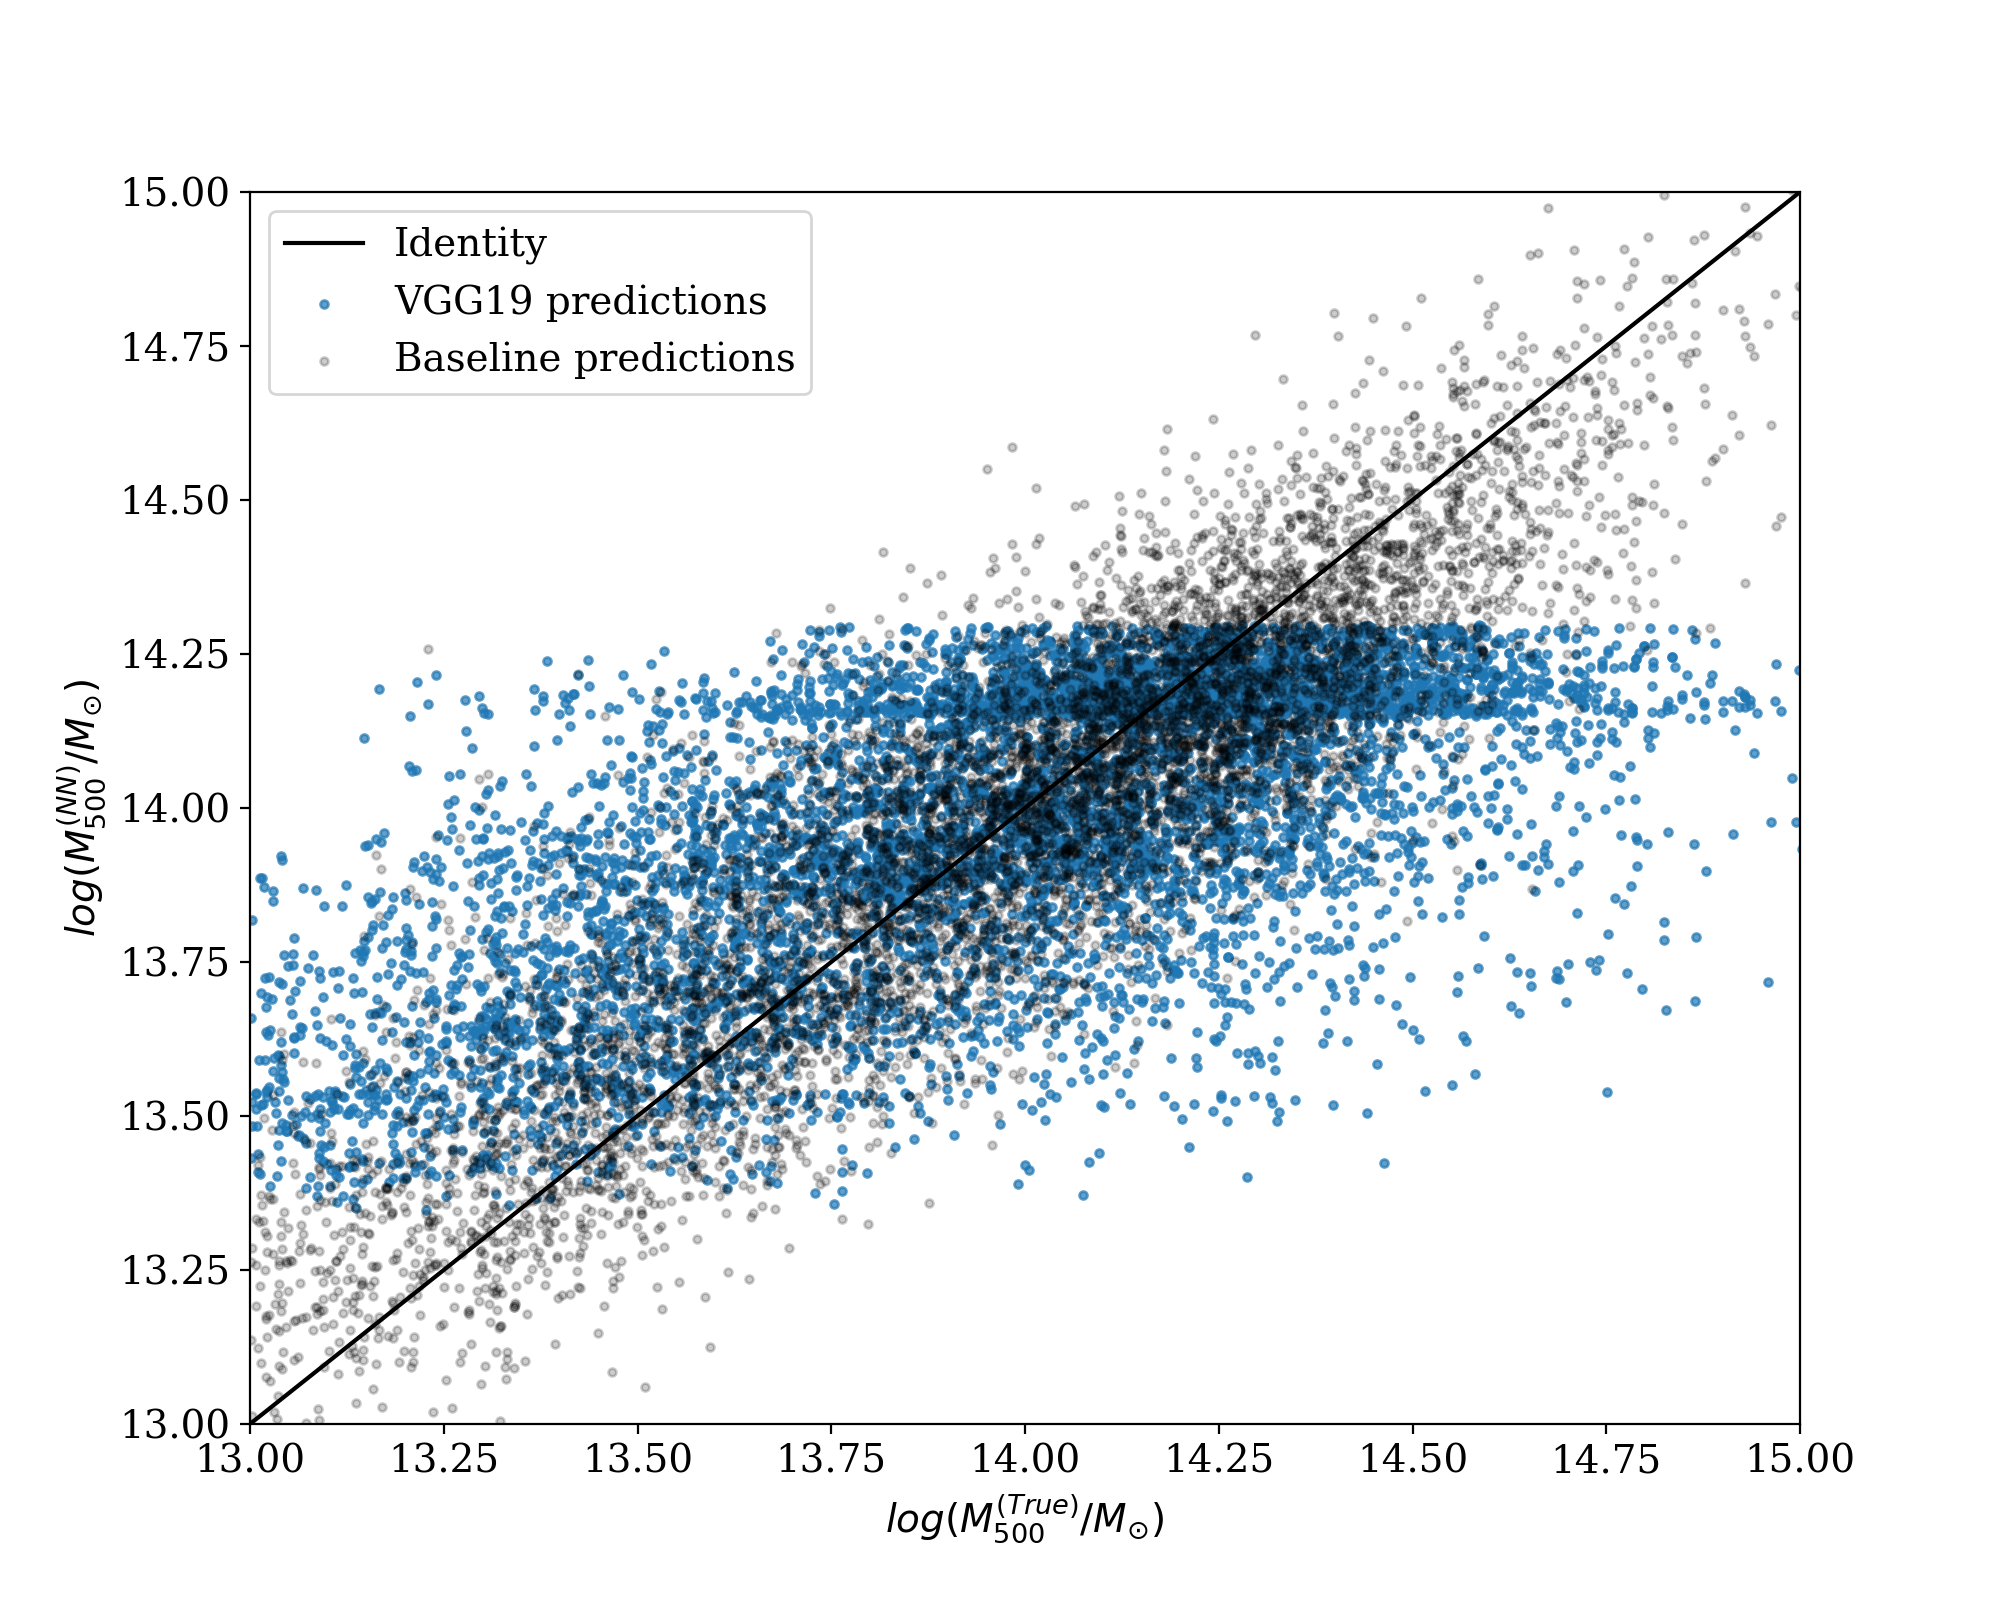
\includegraphics[width=\linewidth]{images/Chapter4/Results/training_VGG19_scatter.png}
    \label{fig:training_VGG19_scatter}
    \caption{VGG19}
\end{subfigure}
\begin{subfigure}{.325\textwidth}
    \centering
    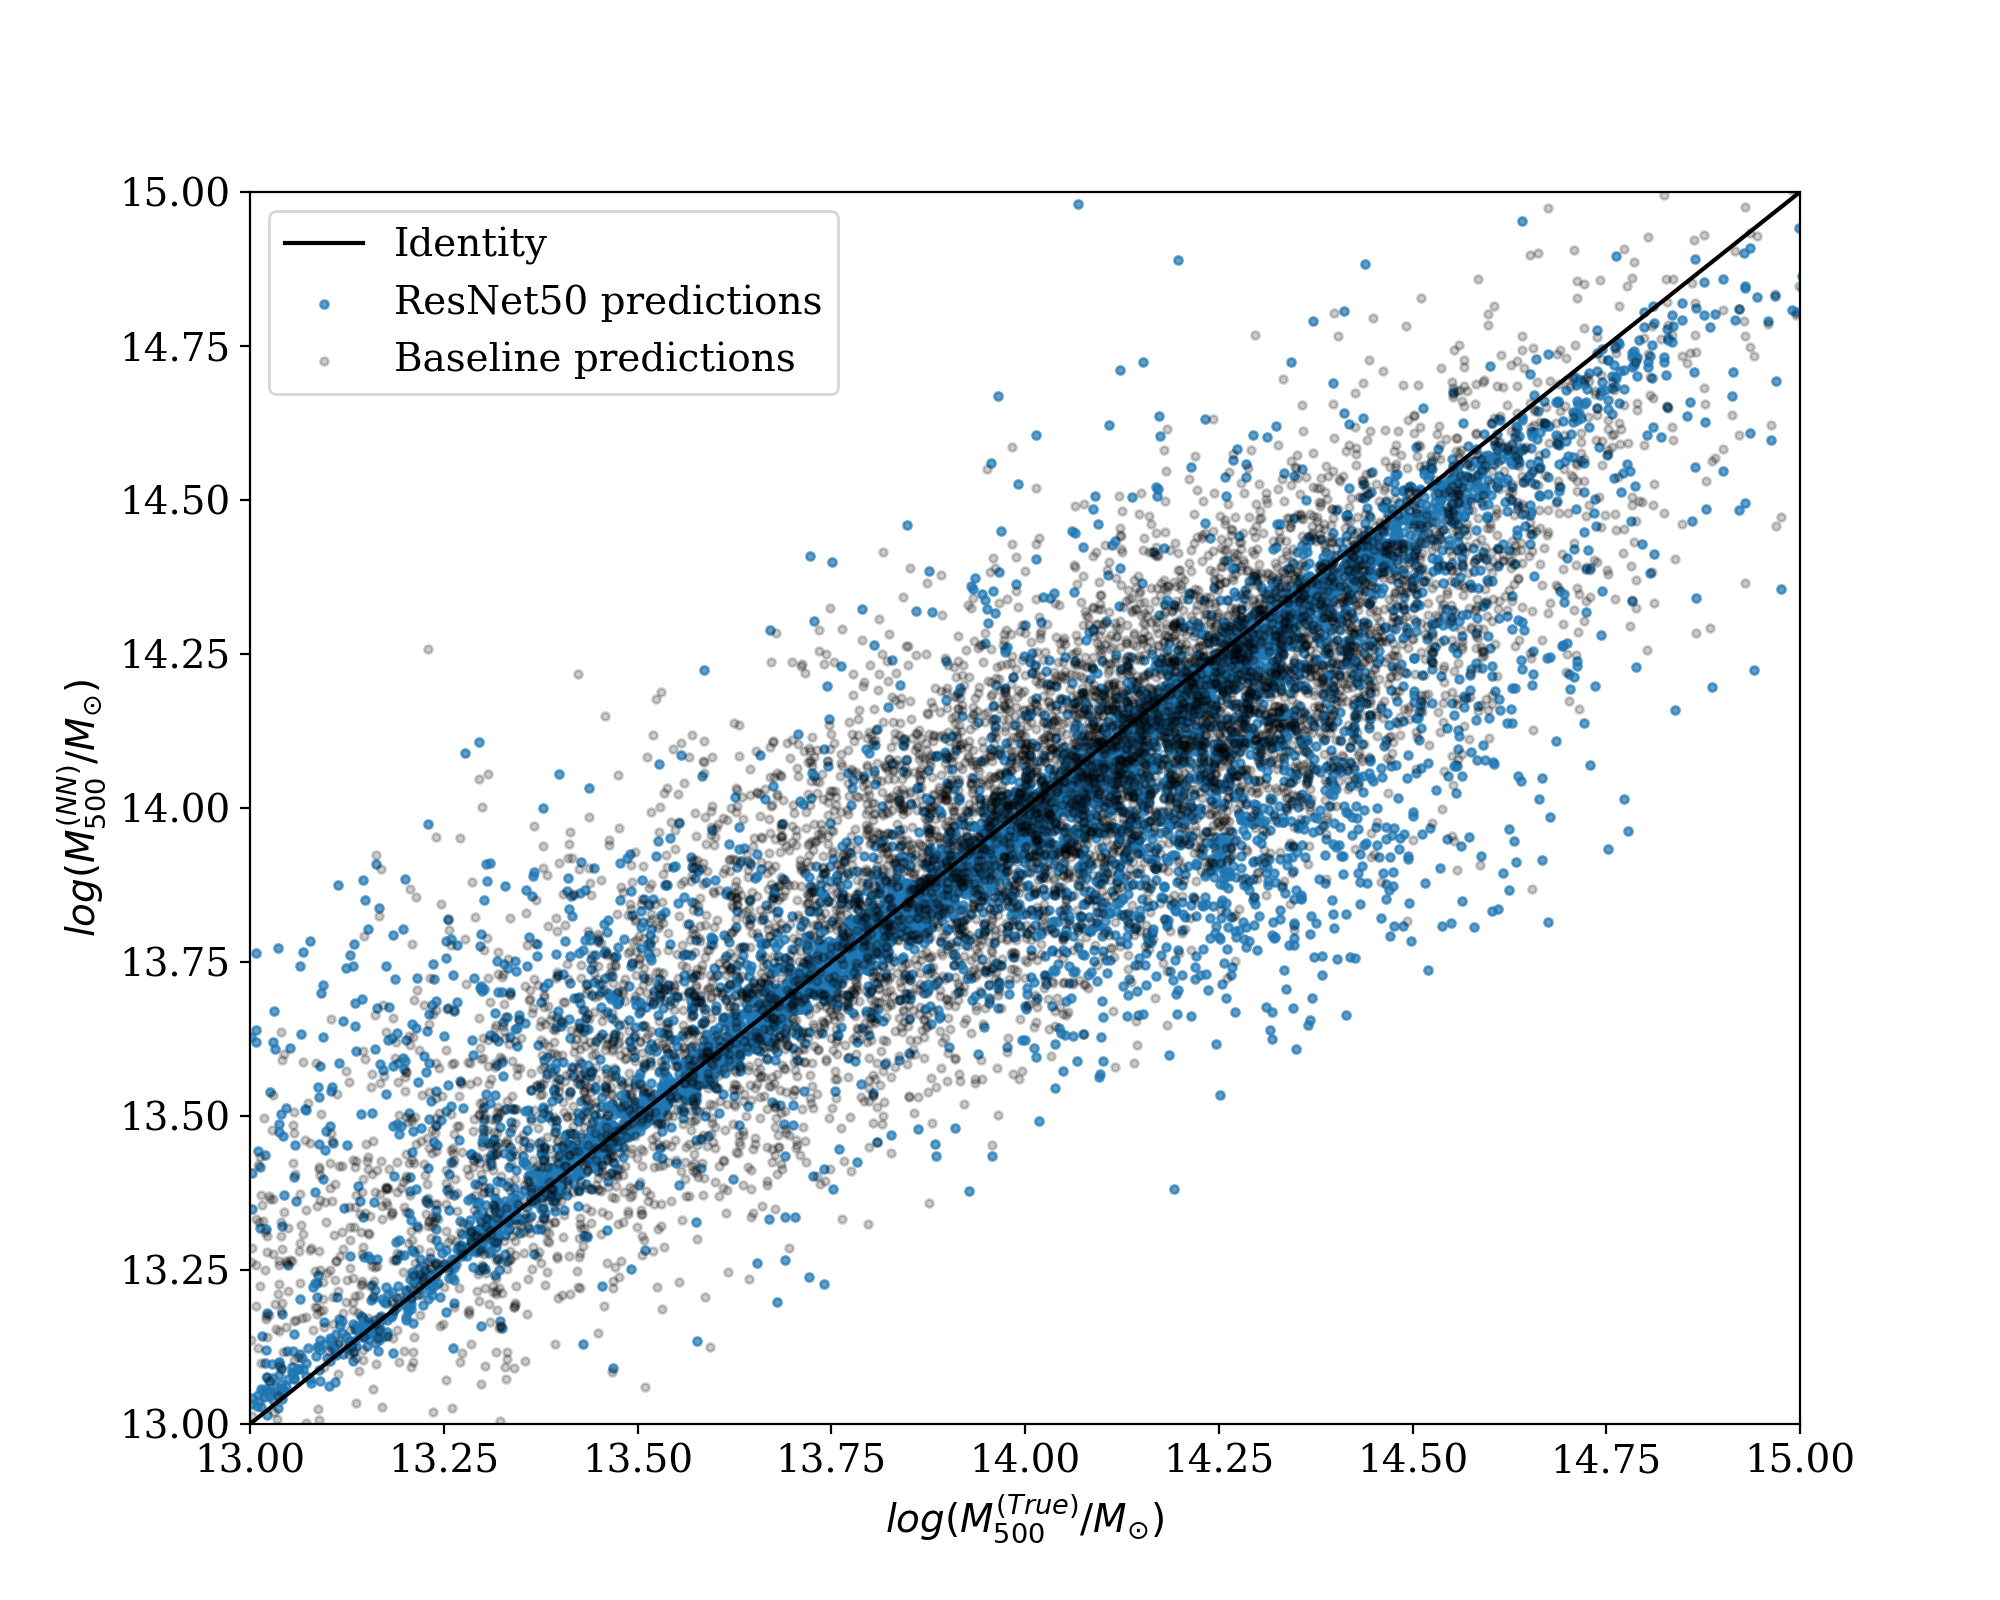
\includegraphics[width=\linewidth]{images/Chapter4/Results/training_ResNet50_scatter.png}
    \label{fig:training_ResNet50_scatter}
    \caption{ResNet50}
\end{subfigure}
\begin{subfigure}{.325\textwidth}
    \centering
    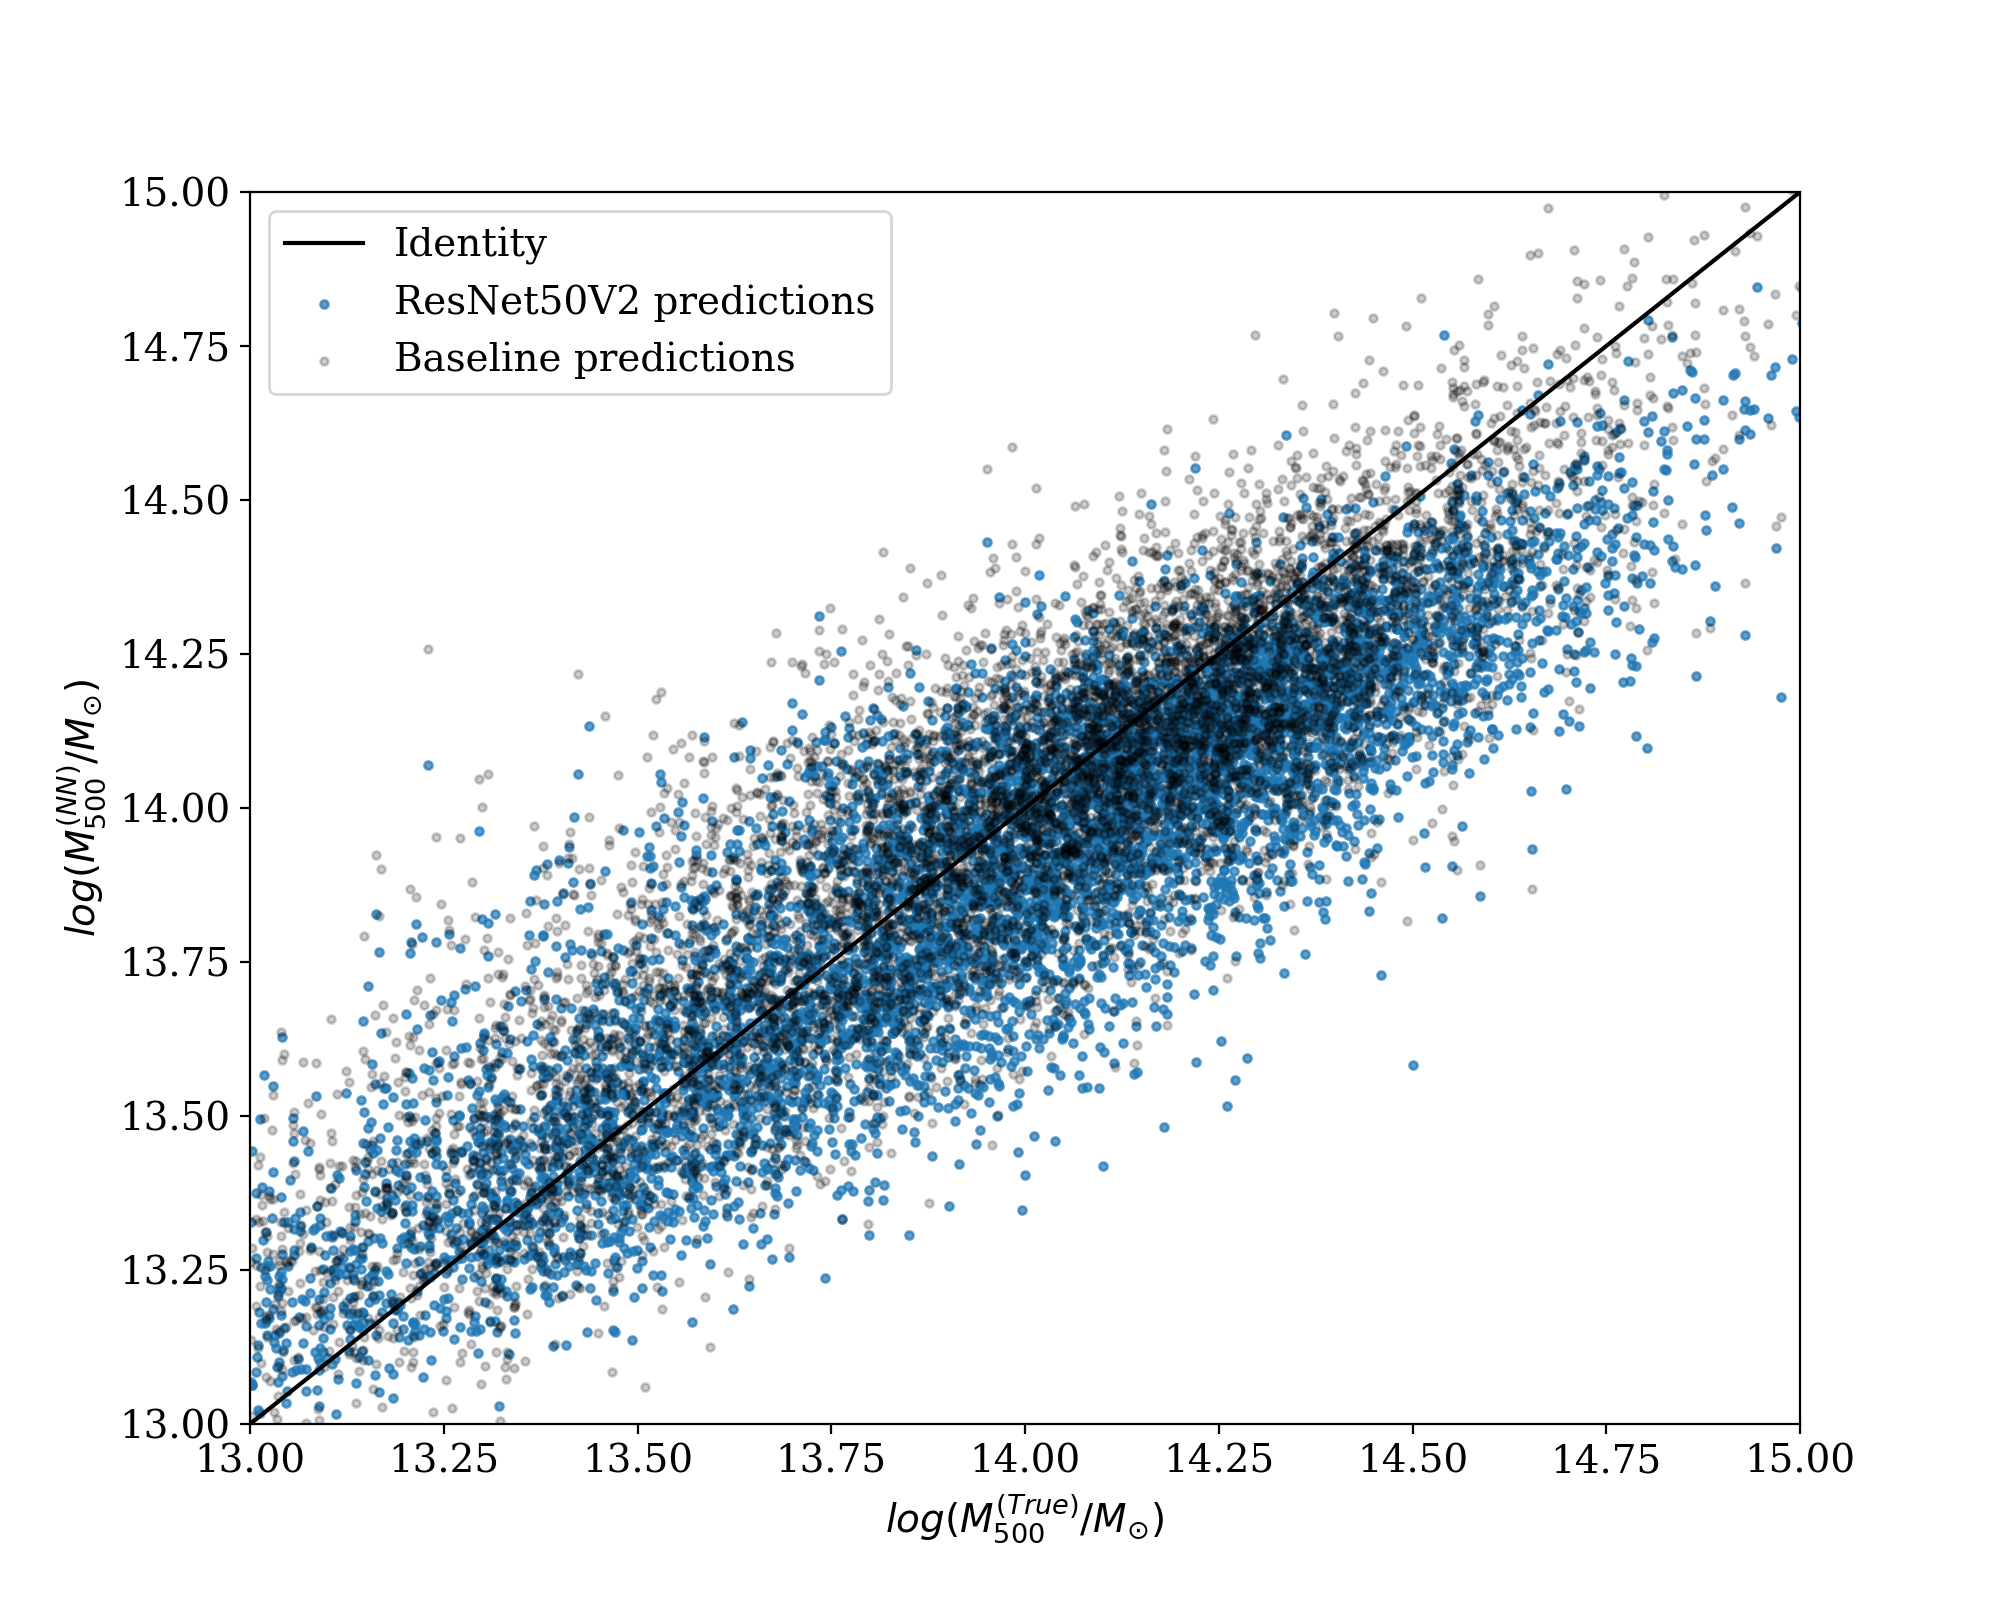
\includegraphics[width=\linewidth]{images/Chapter4/Results/training_ResNet50V2_scatter.png}
    \label{fig:training_ResNet50V2_scatter}
    \caption{ResNet50V2}
\end{subfigure}
\begin{subfigure}{.325\textwidth}
    \centering
    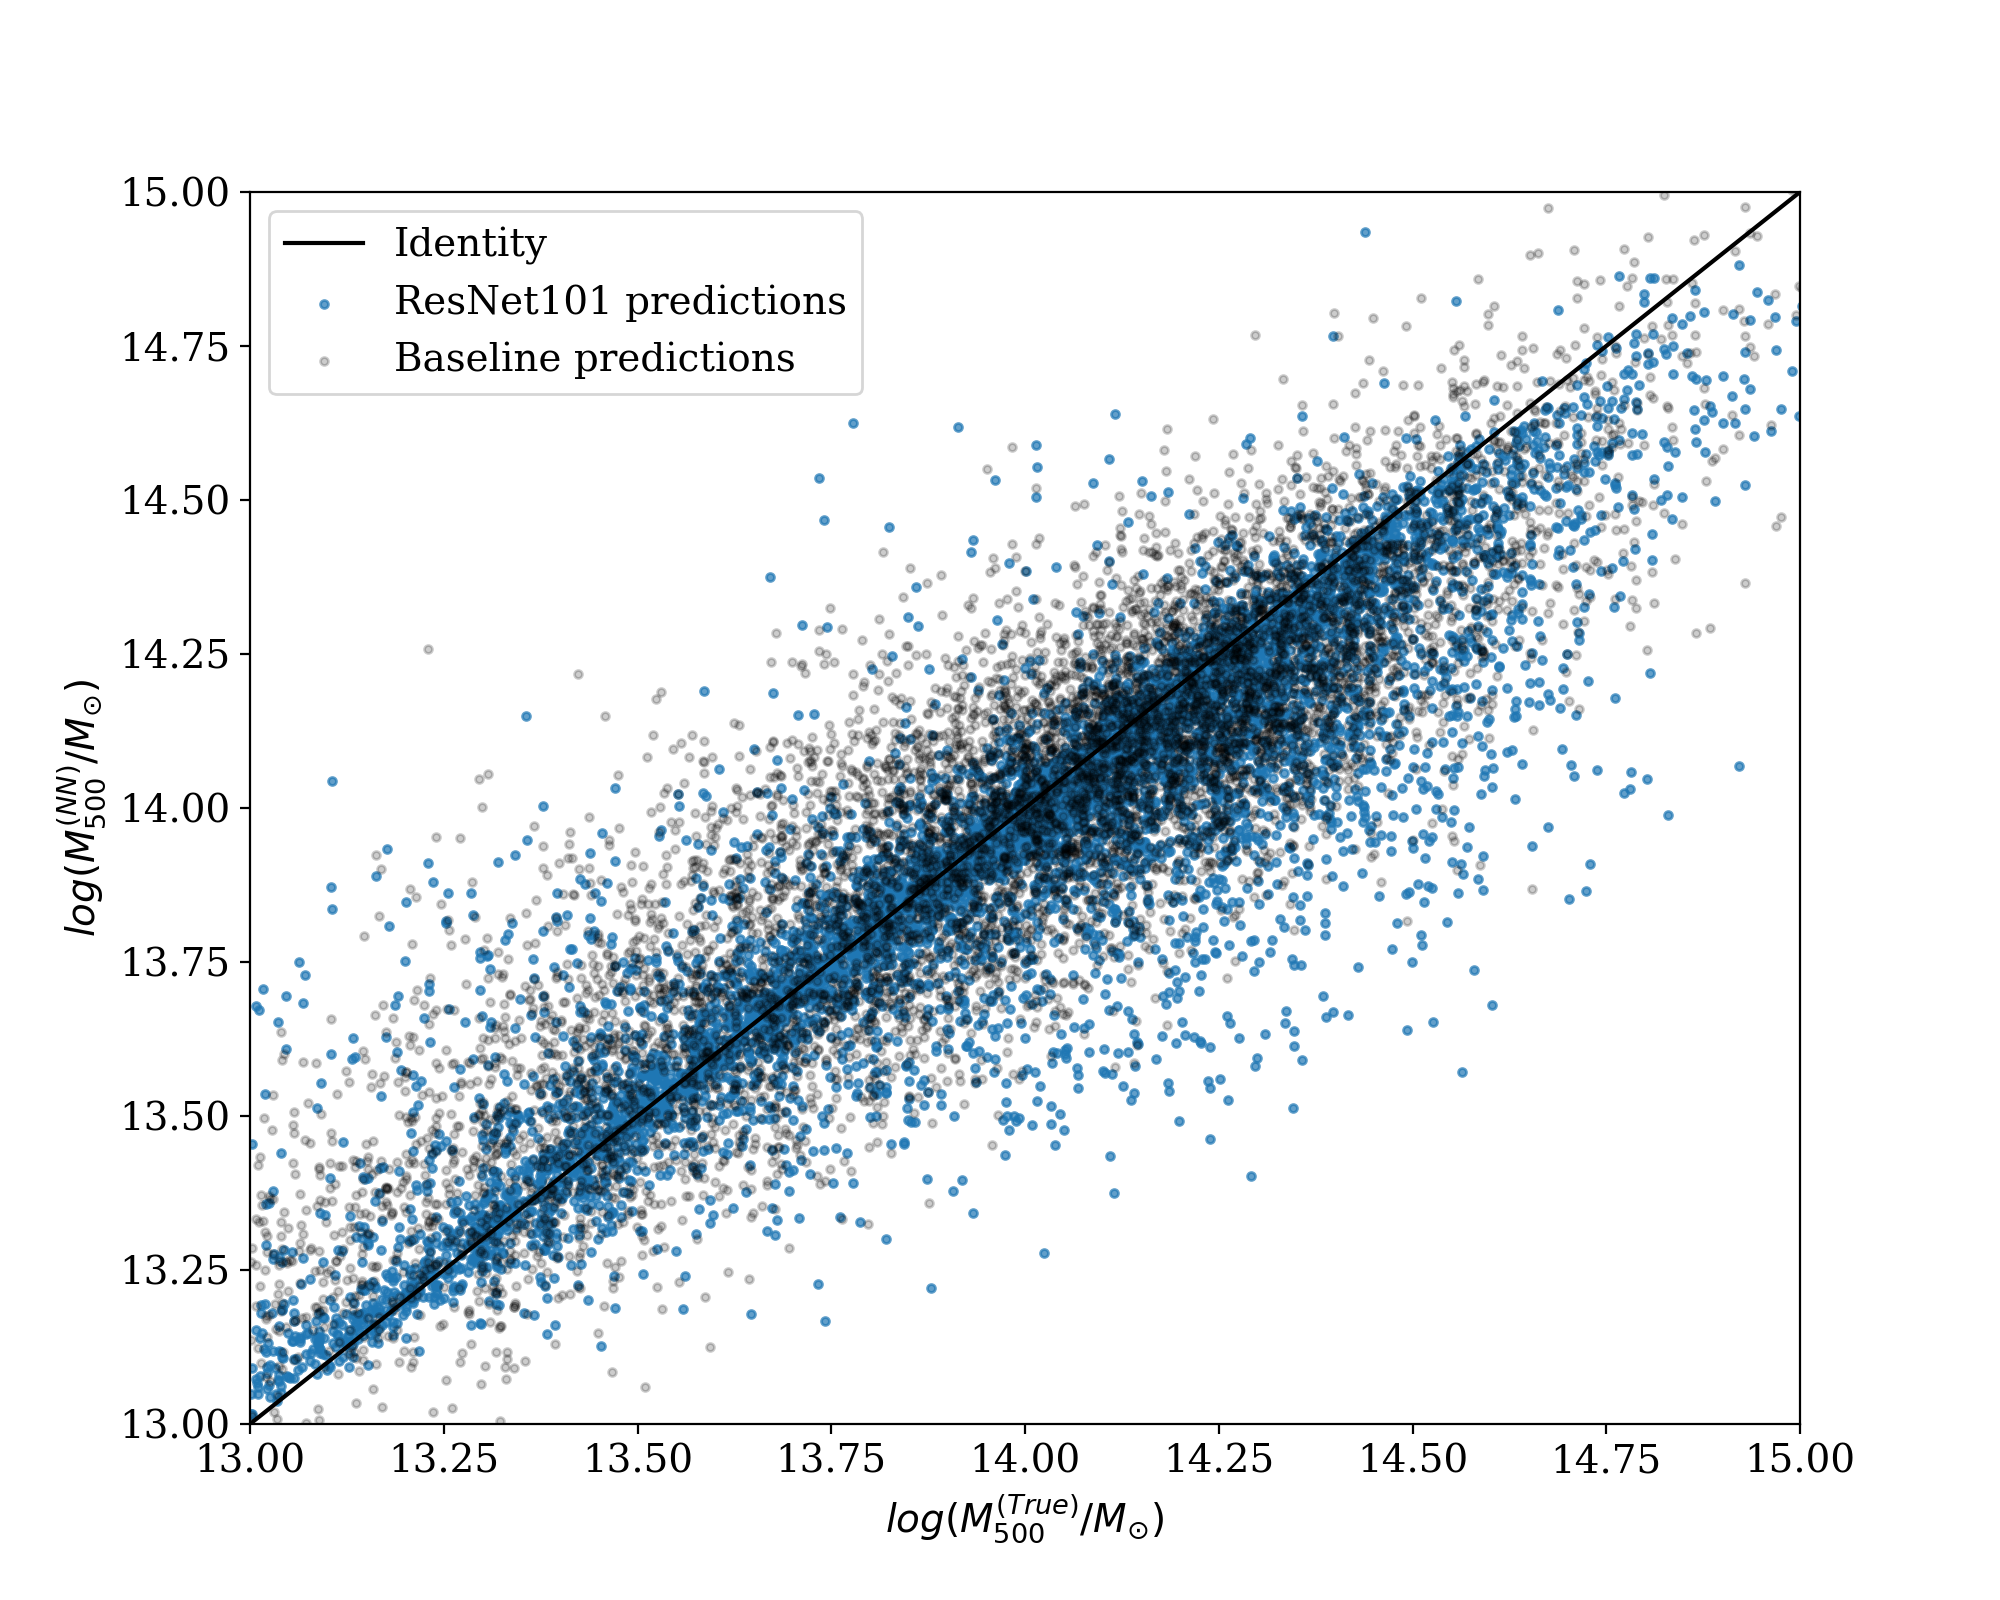
\includegraphics[width=\linewidth]{images/Chapter4/Results/training_ResNet101_scatter.png}
    \label{fig:training_ResNet101_scatter}
    \caption{ResNet101}
\end{subfigure}
\begin{subfigure}{.325\textwidth}
    \centering
    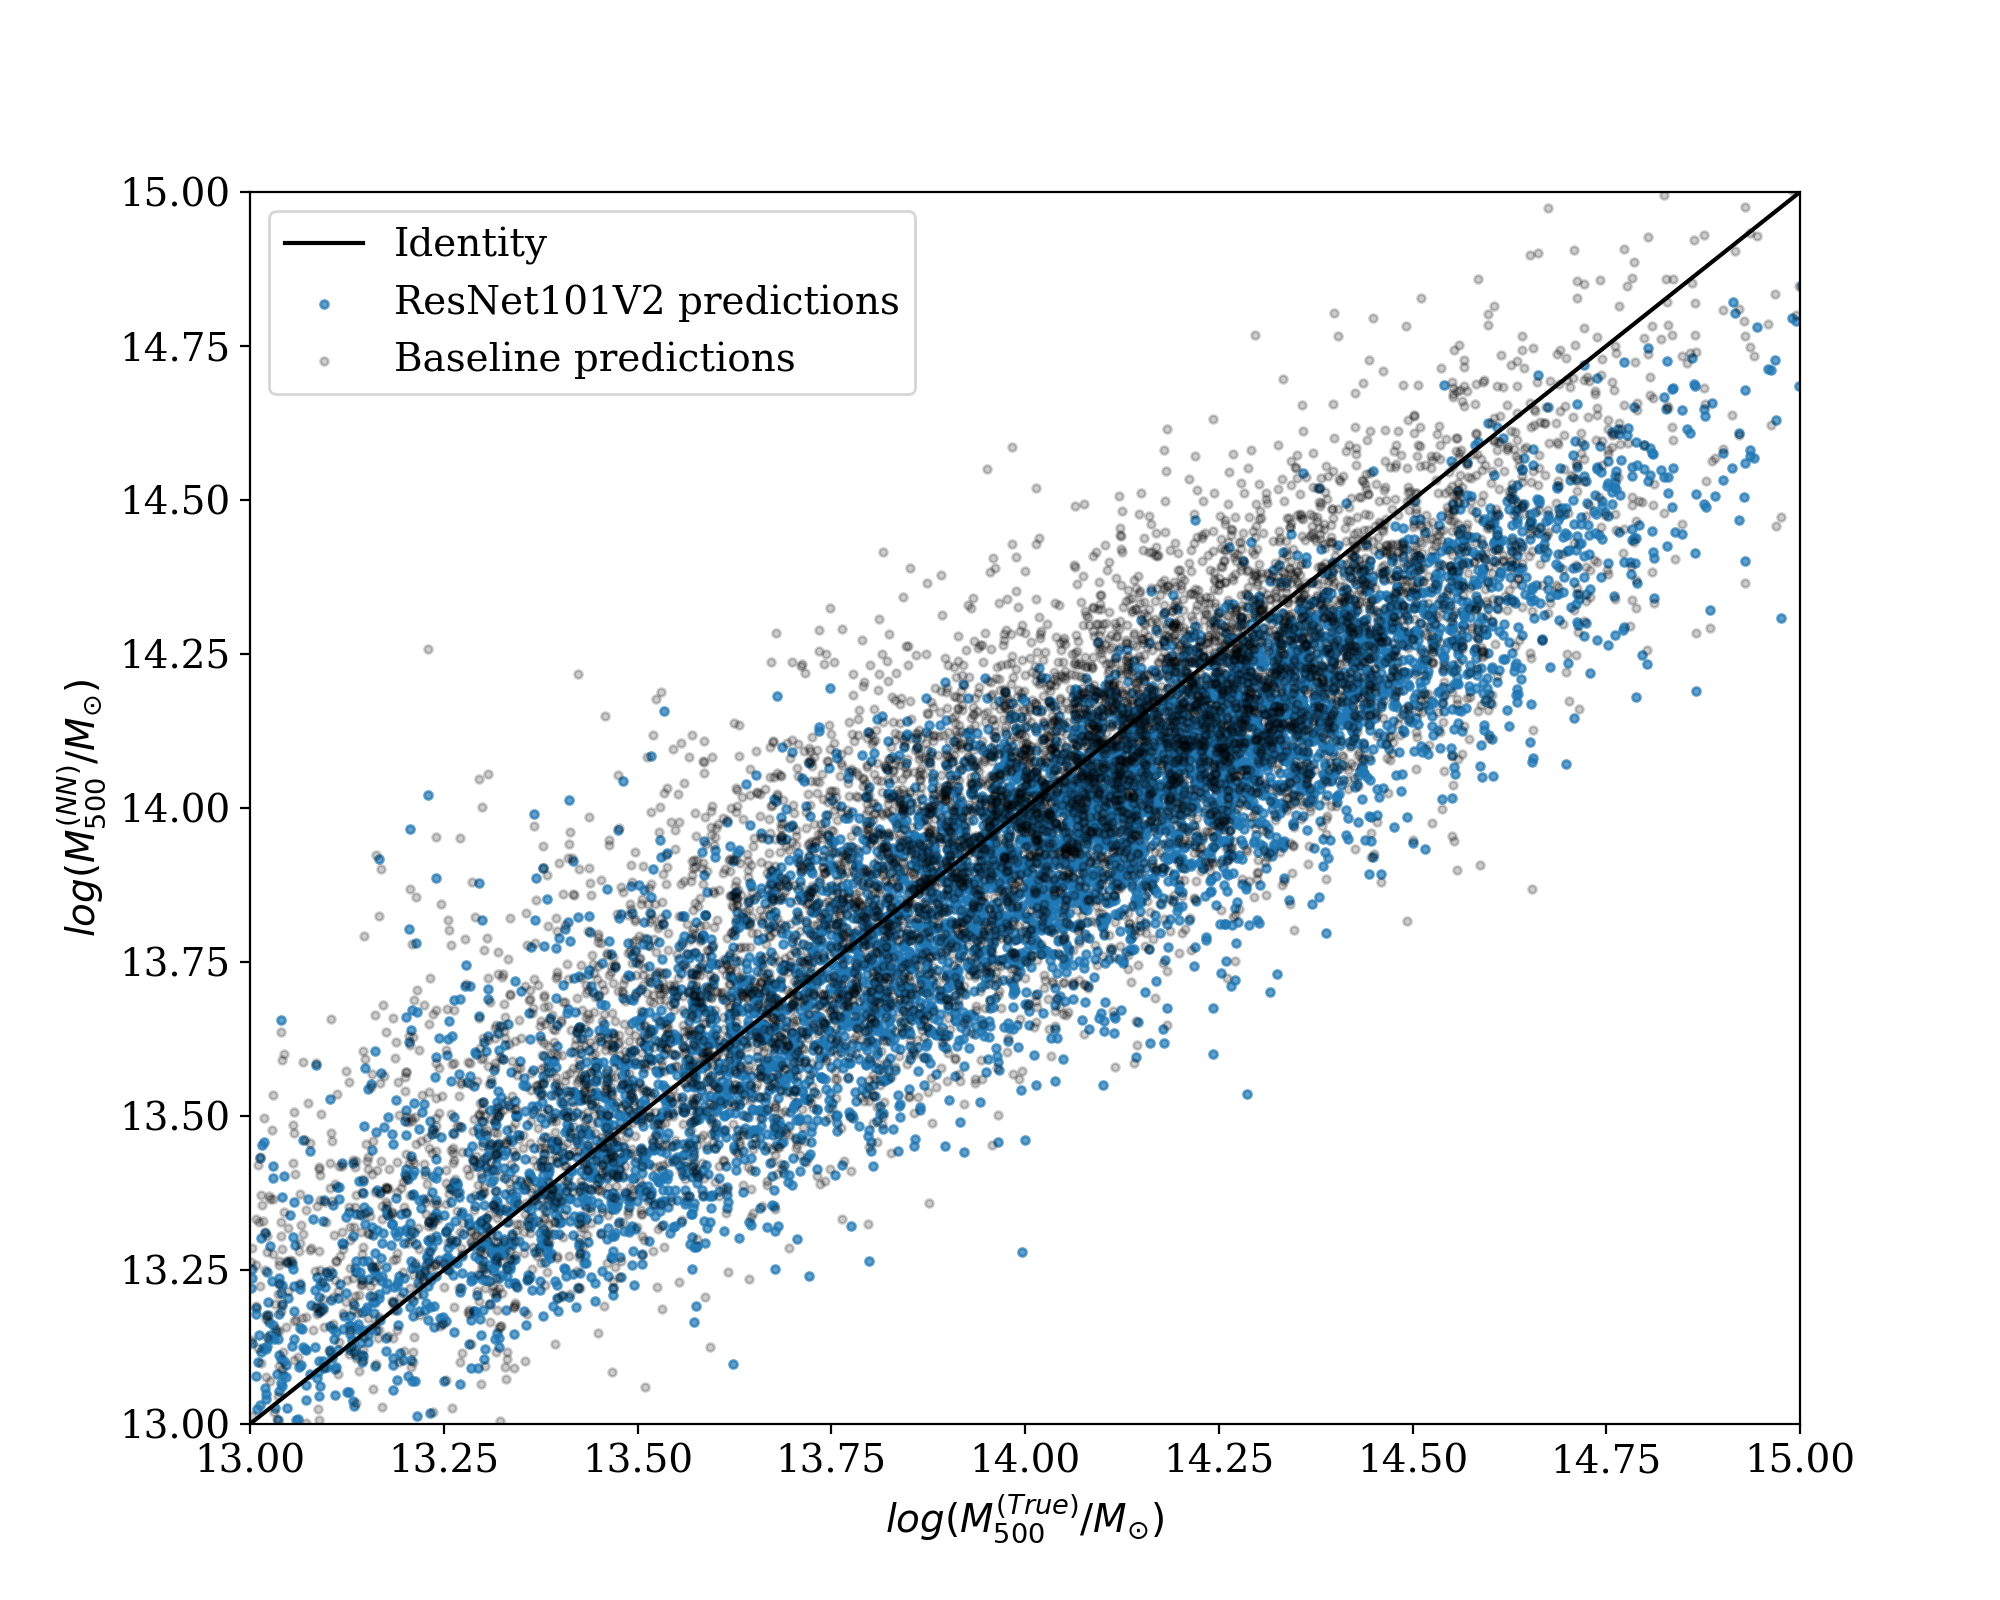
\includegraphics[width=\linewidth]{images/Chapter4/Results/training_ResNet101V2_scatter.png}
    \label{fig:training_ResNet101V2_scatter}
    \caption{ResNet101V2}
\end{subfigure}
\begin{subfigure}{.325\textwidth}
    \centering
    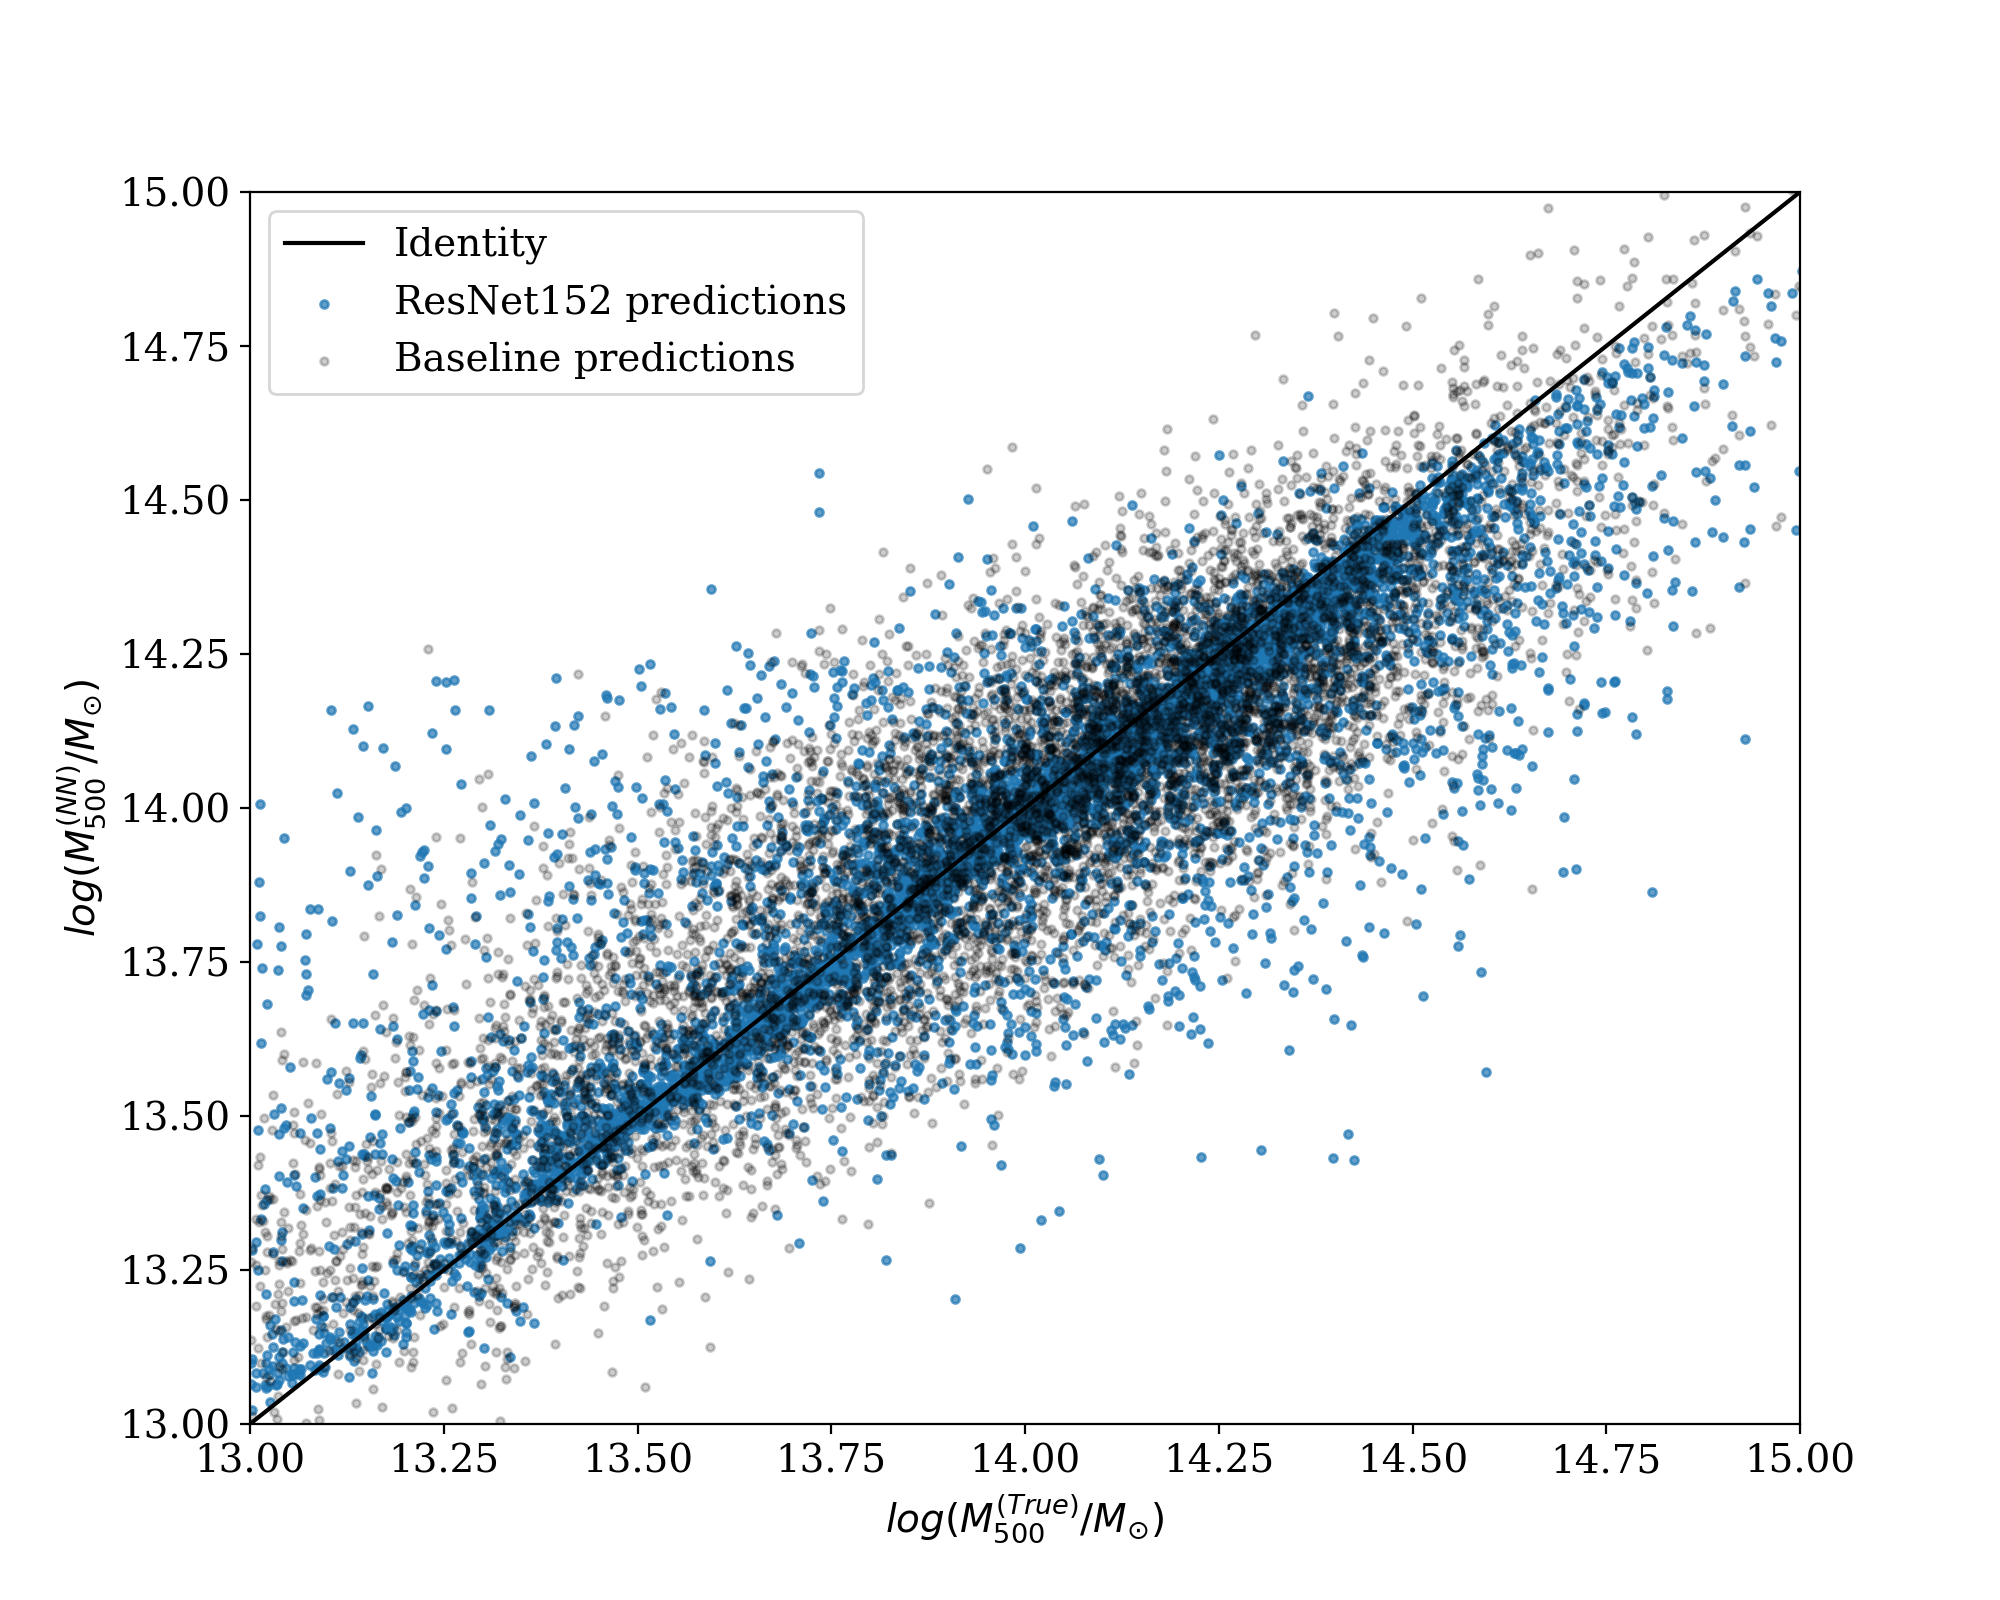
\includegraphics[width=\linewidth]{images/Chapter4/Results/training_ResNet152_scatter.png}
    \label{fig:training_ResNet152_scatter}
    \caption{ResNet152}
\end{subfigure}
\begin{subfigure}{.325\textwidth}
    \centering
    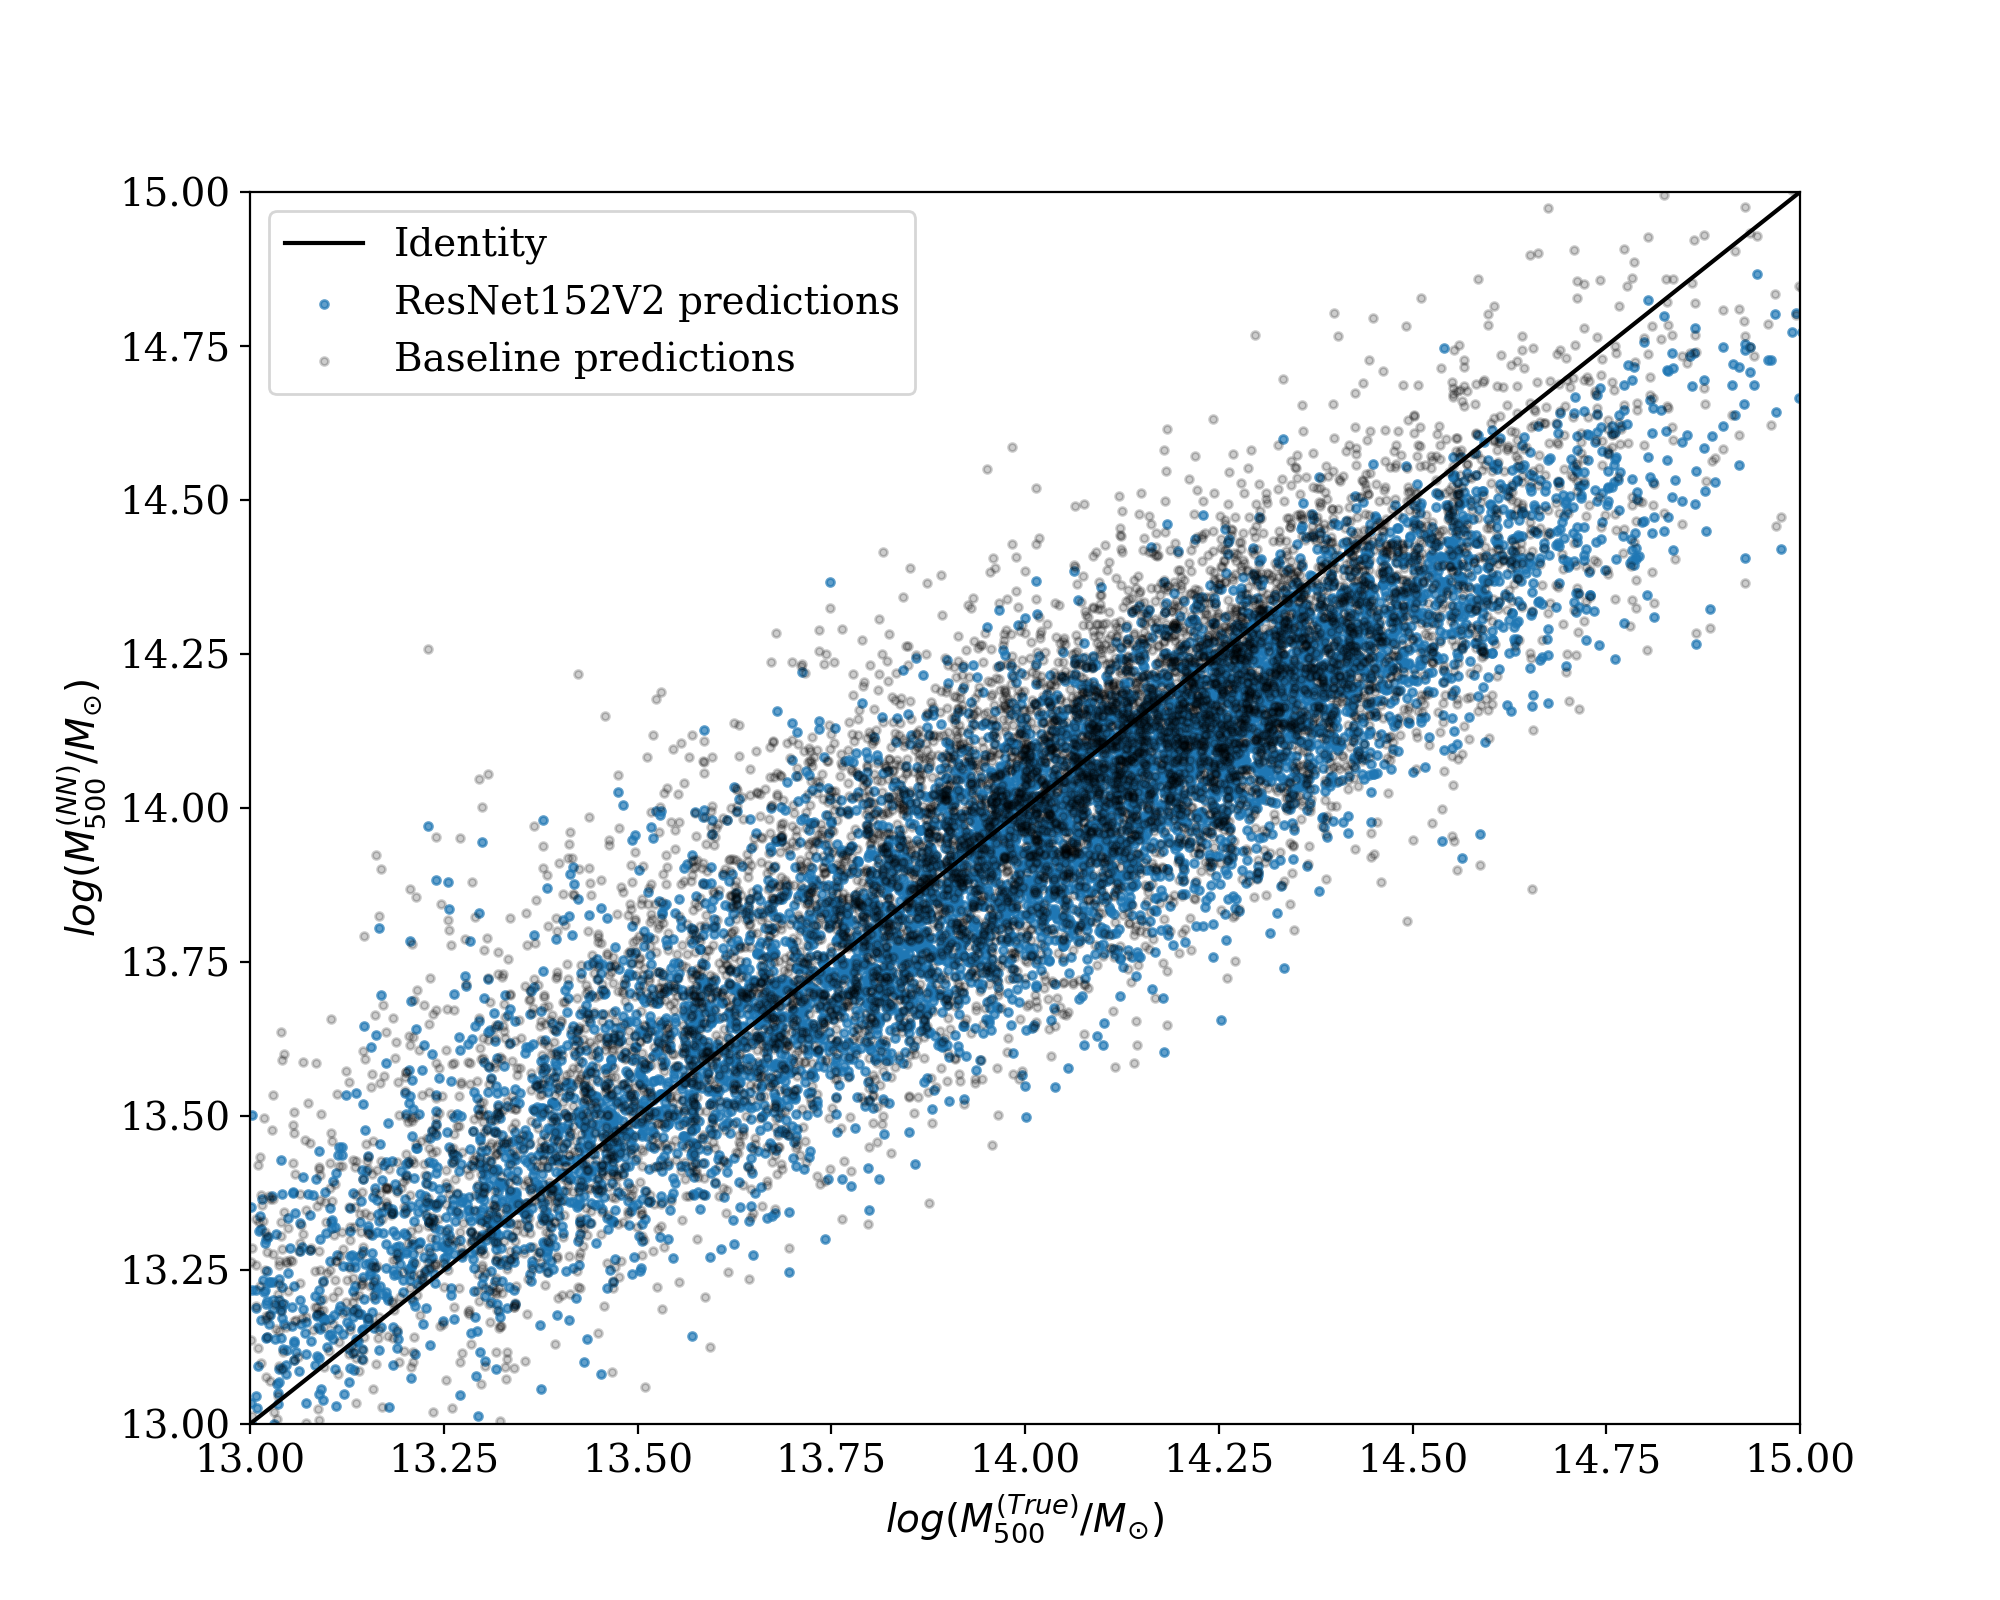
\includegraphics[width=\linewidth]{images/Chapter4/Results/training_ResNet152V2_scatter.png}
    \label{fig:training_ResNet152V2_scatter}
    \caption{ResNet152V2}
\end{subfigure}
\begin{subfigure}{.325\textwidth}
    \centering
    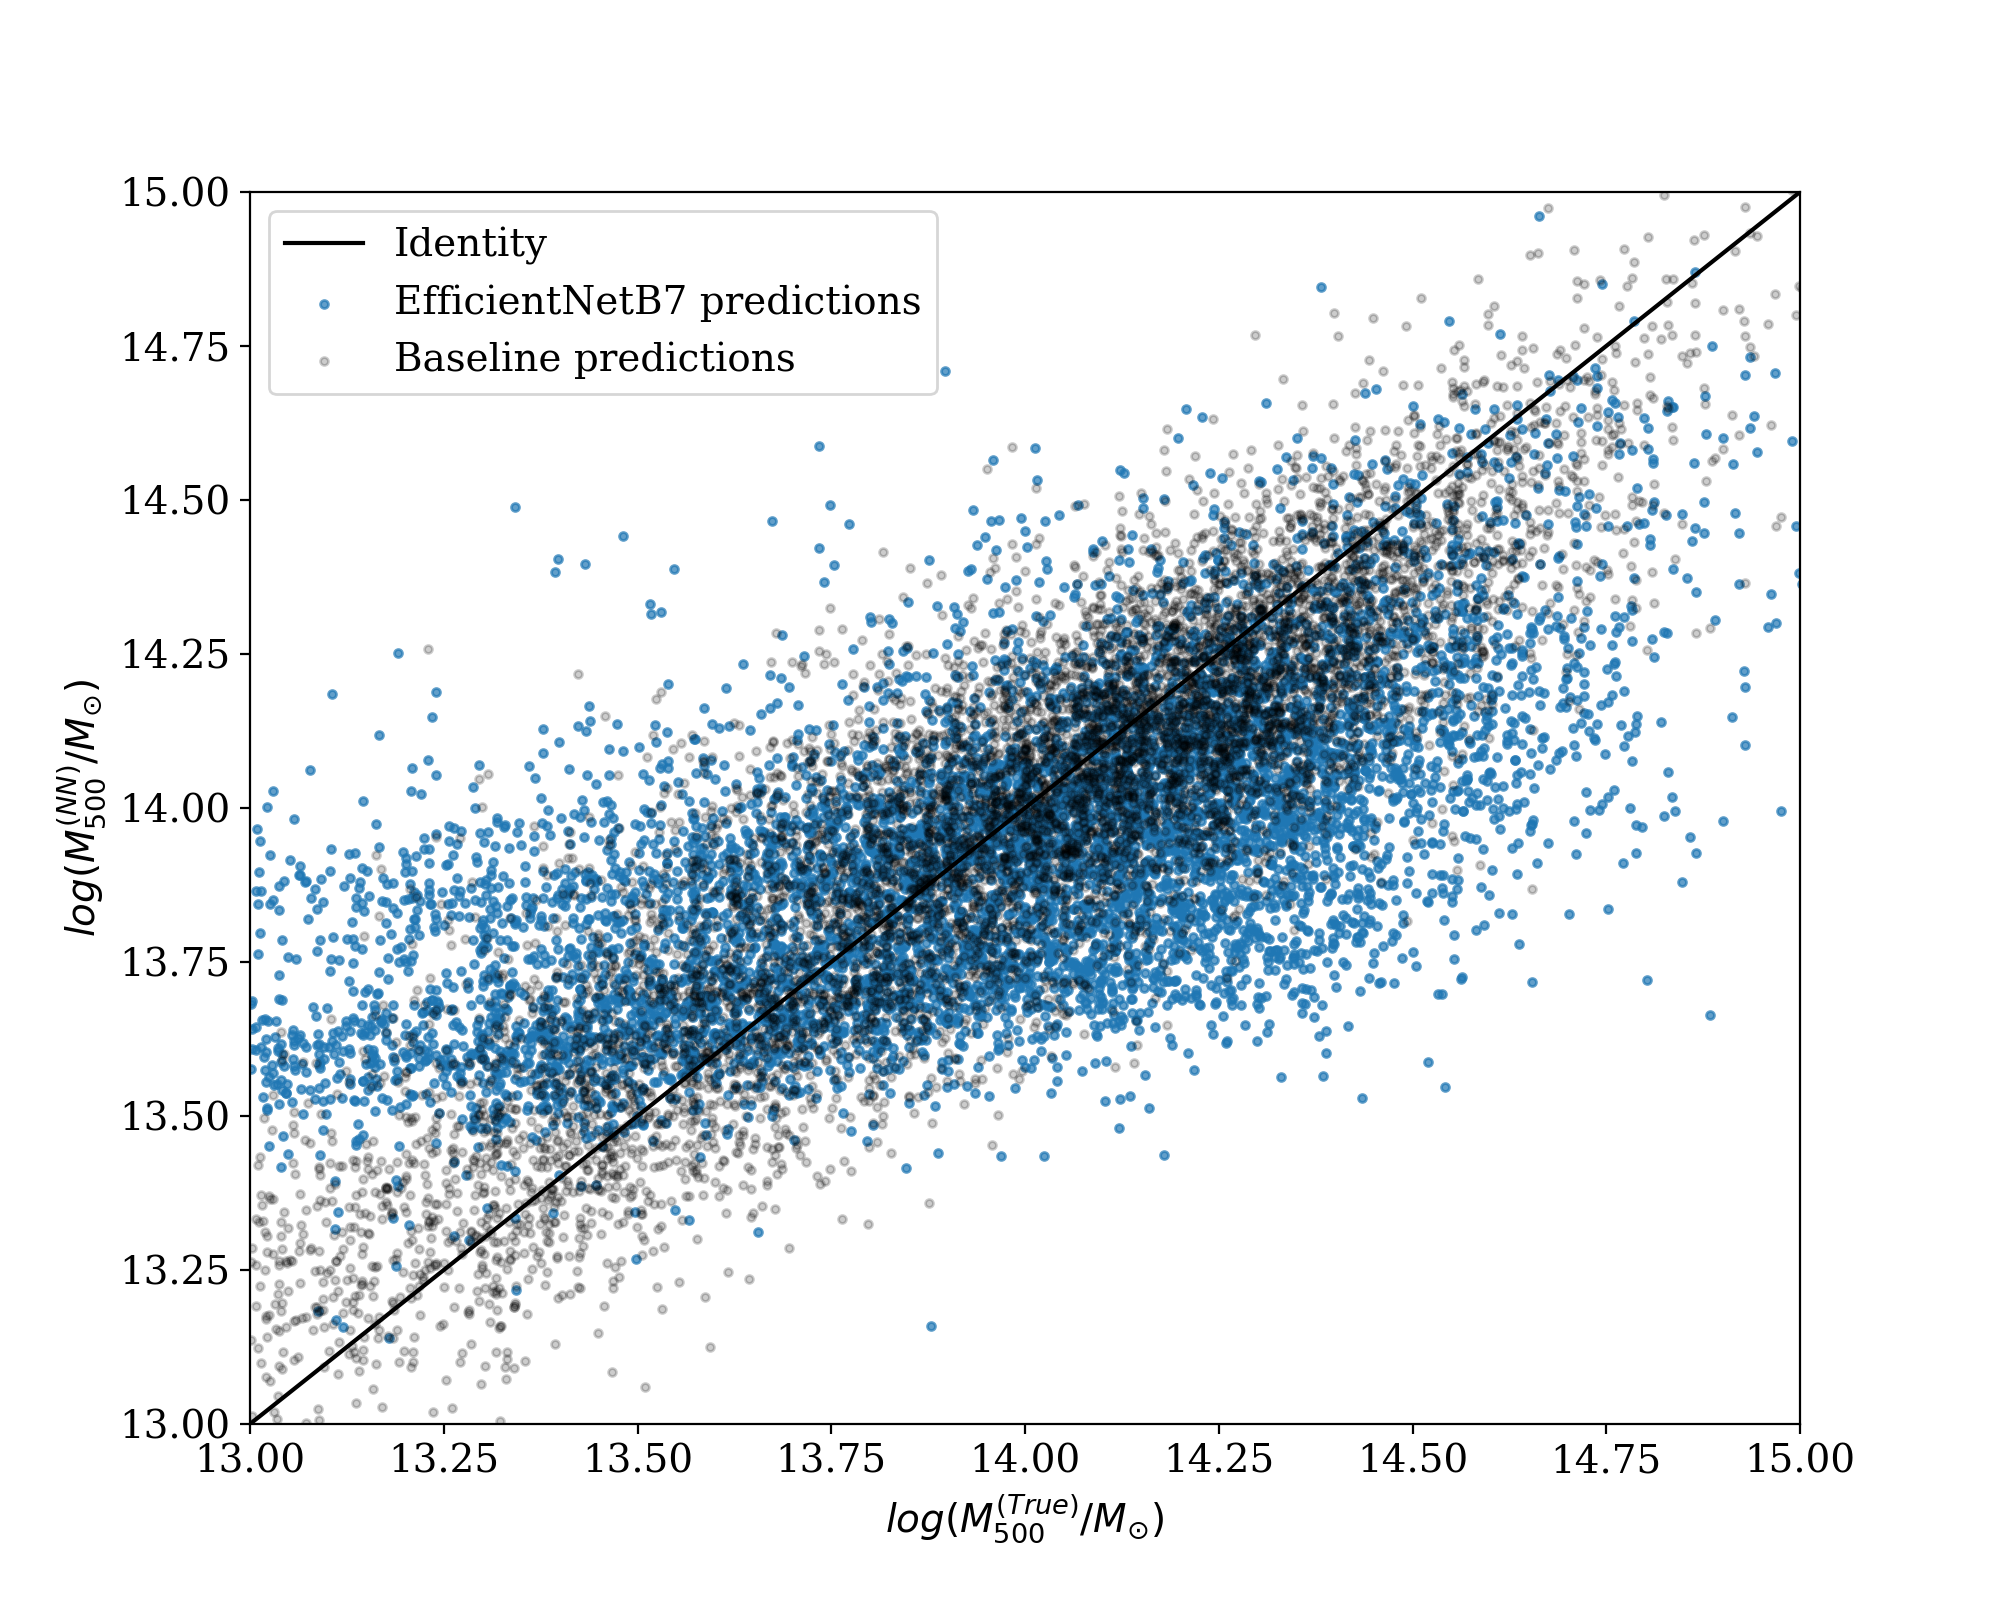
\includegraphics[width=\linewidth]{images/Chapter4/Results/training_EfficientNetB7_scatter.png}
    \label{fig:training_EfficientNetB7_scatter}
    \caption{EfficientNetB7}
\end{subfigure}
\caption{Comparison between each deep model's best predictions (\textit{blue}) and the best predictions from the basic CNN (\textit{grey}) on the training set.}
\end{figure}

\begin{figure}[H]
\centering
\begin{subfigure}{.325\textwidth}
    \centering
    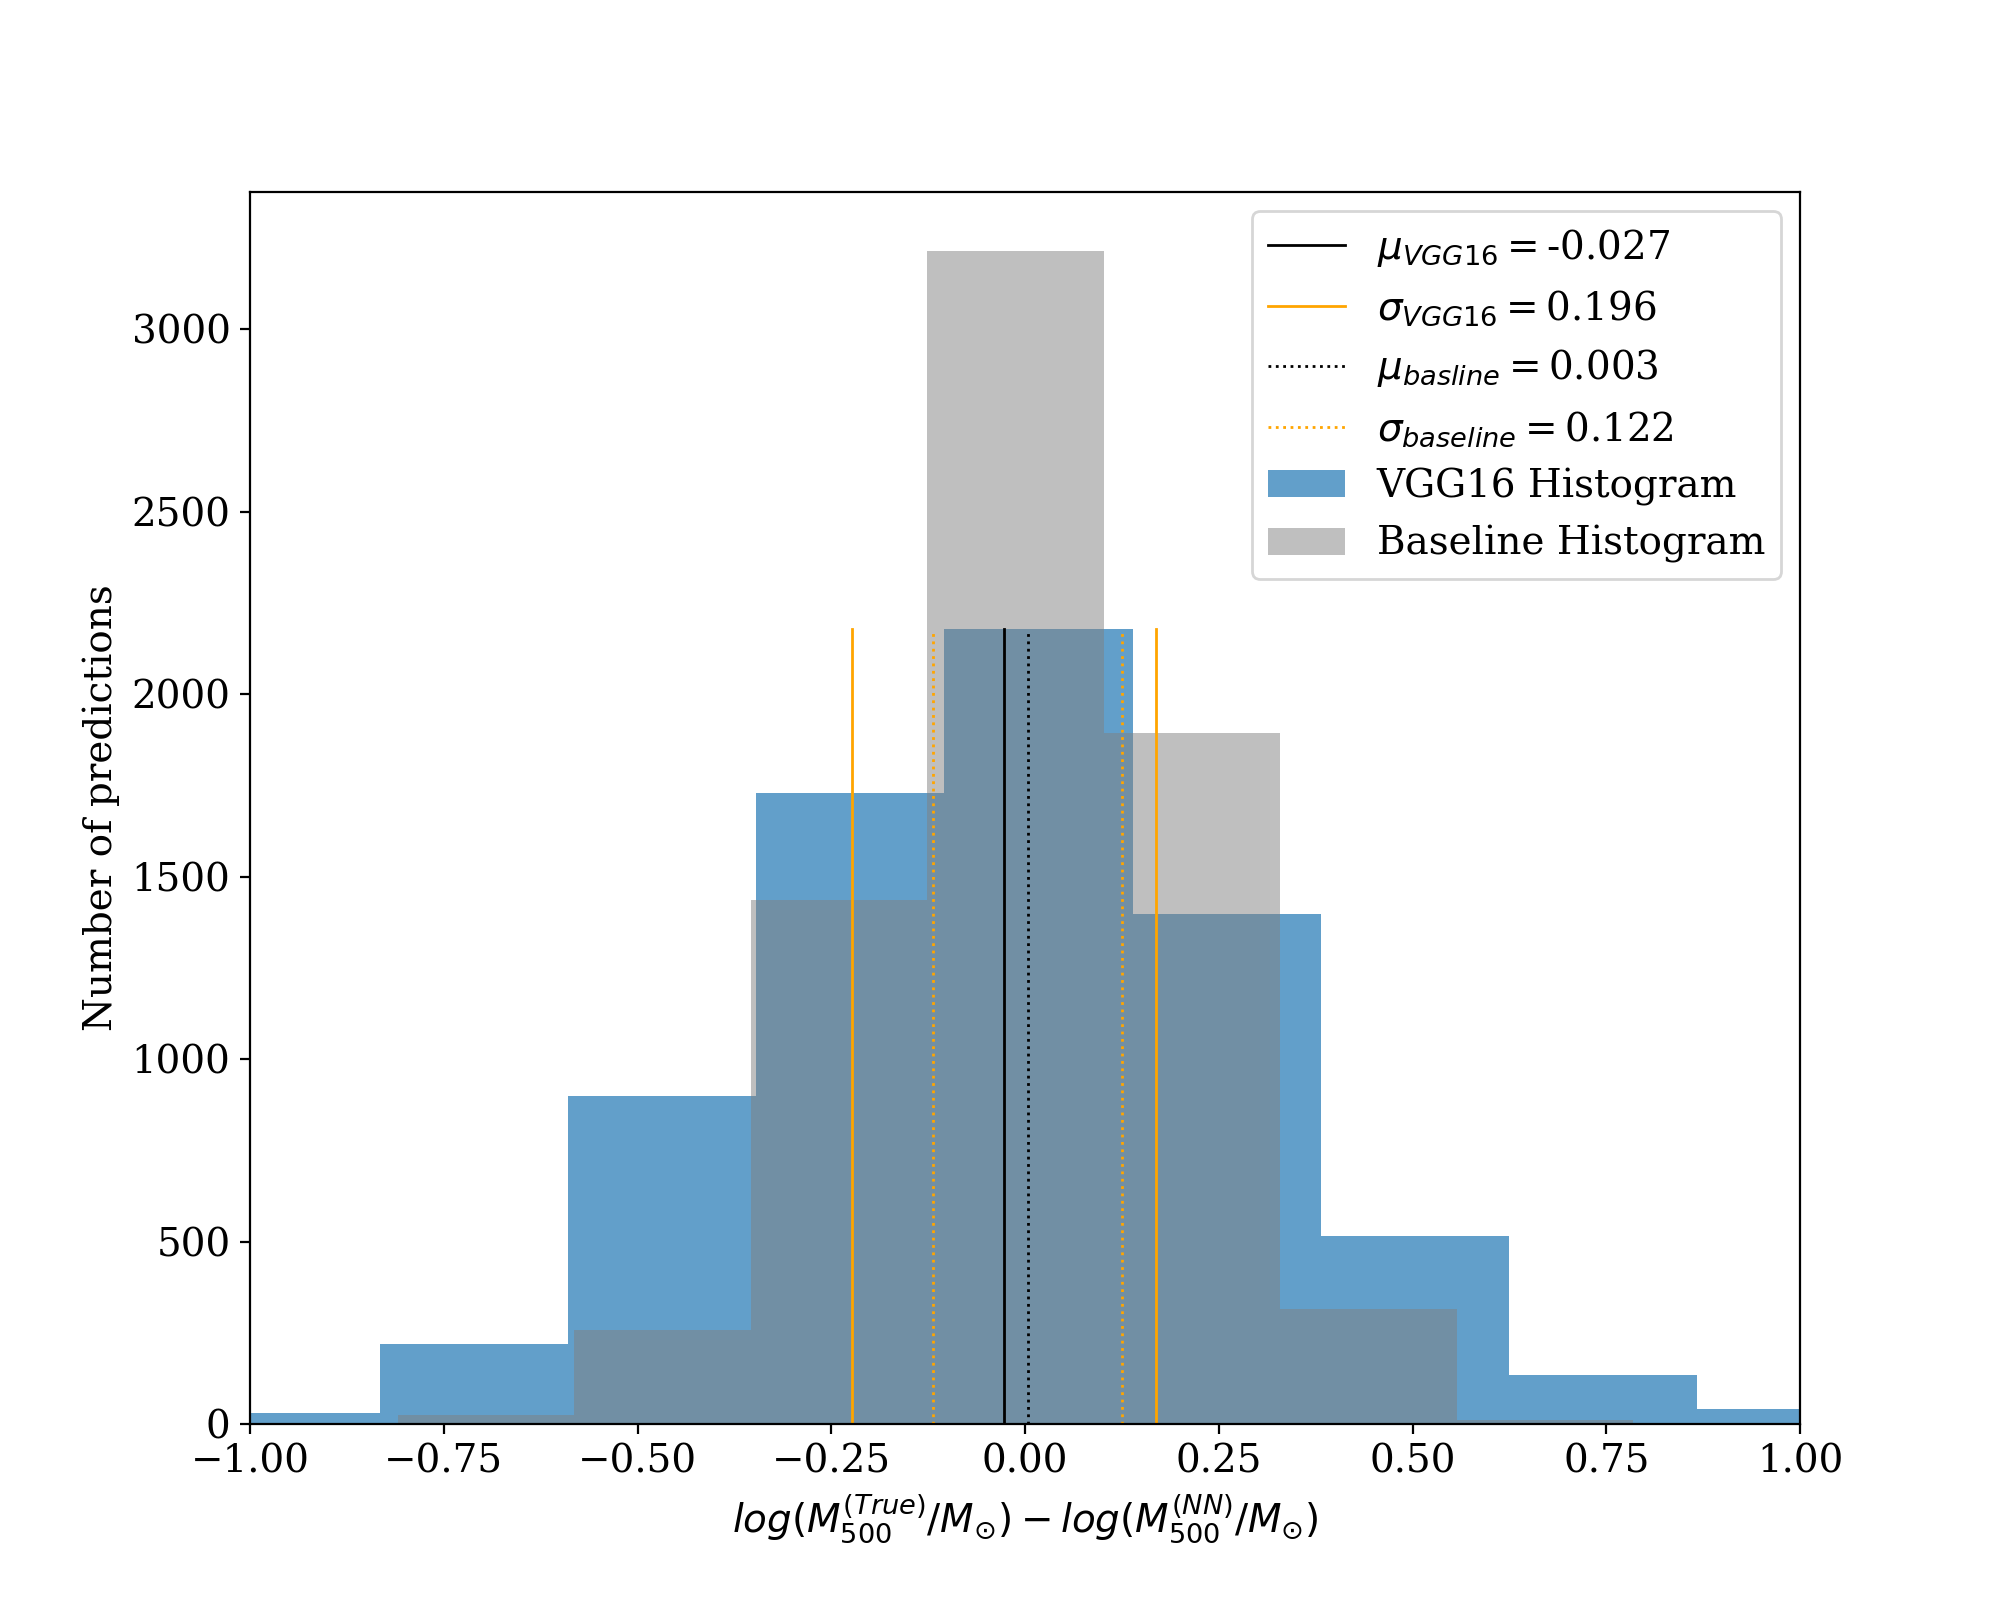
\includegraphics[width=\linewidth]{images/Chapter4/Results/training_VGG16_hist.png}
    \label{fig:training_VGG16_hist}
    \caption{VGG16}
\end{subfigure}
\begin{subfigure}{.325\textwidth}
    \centering
    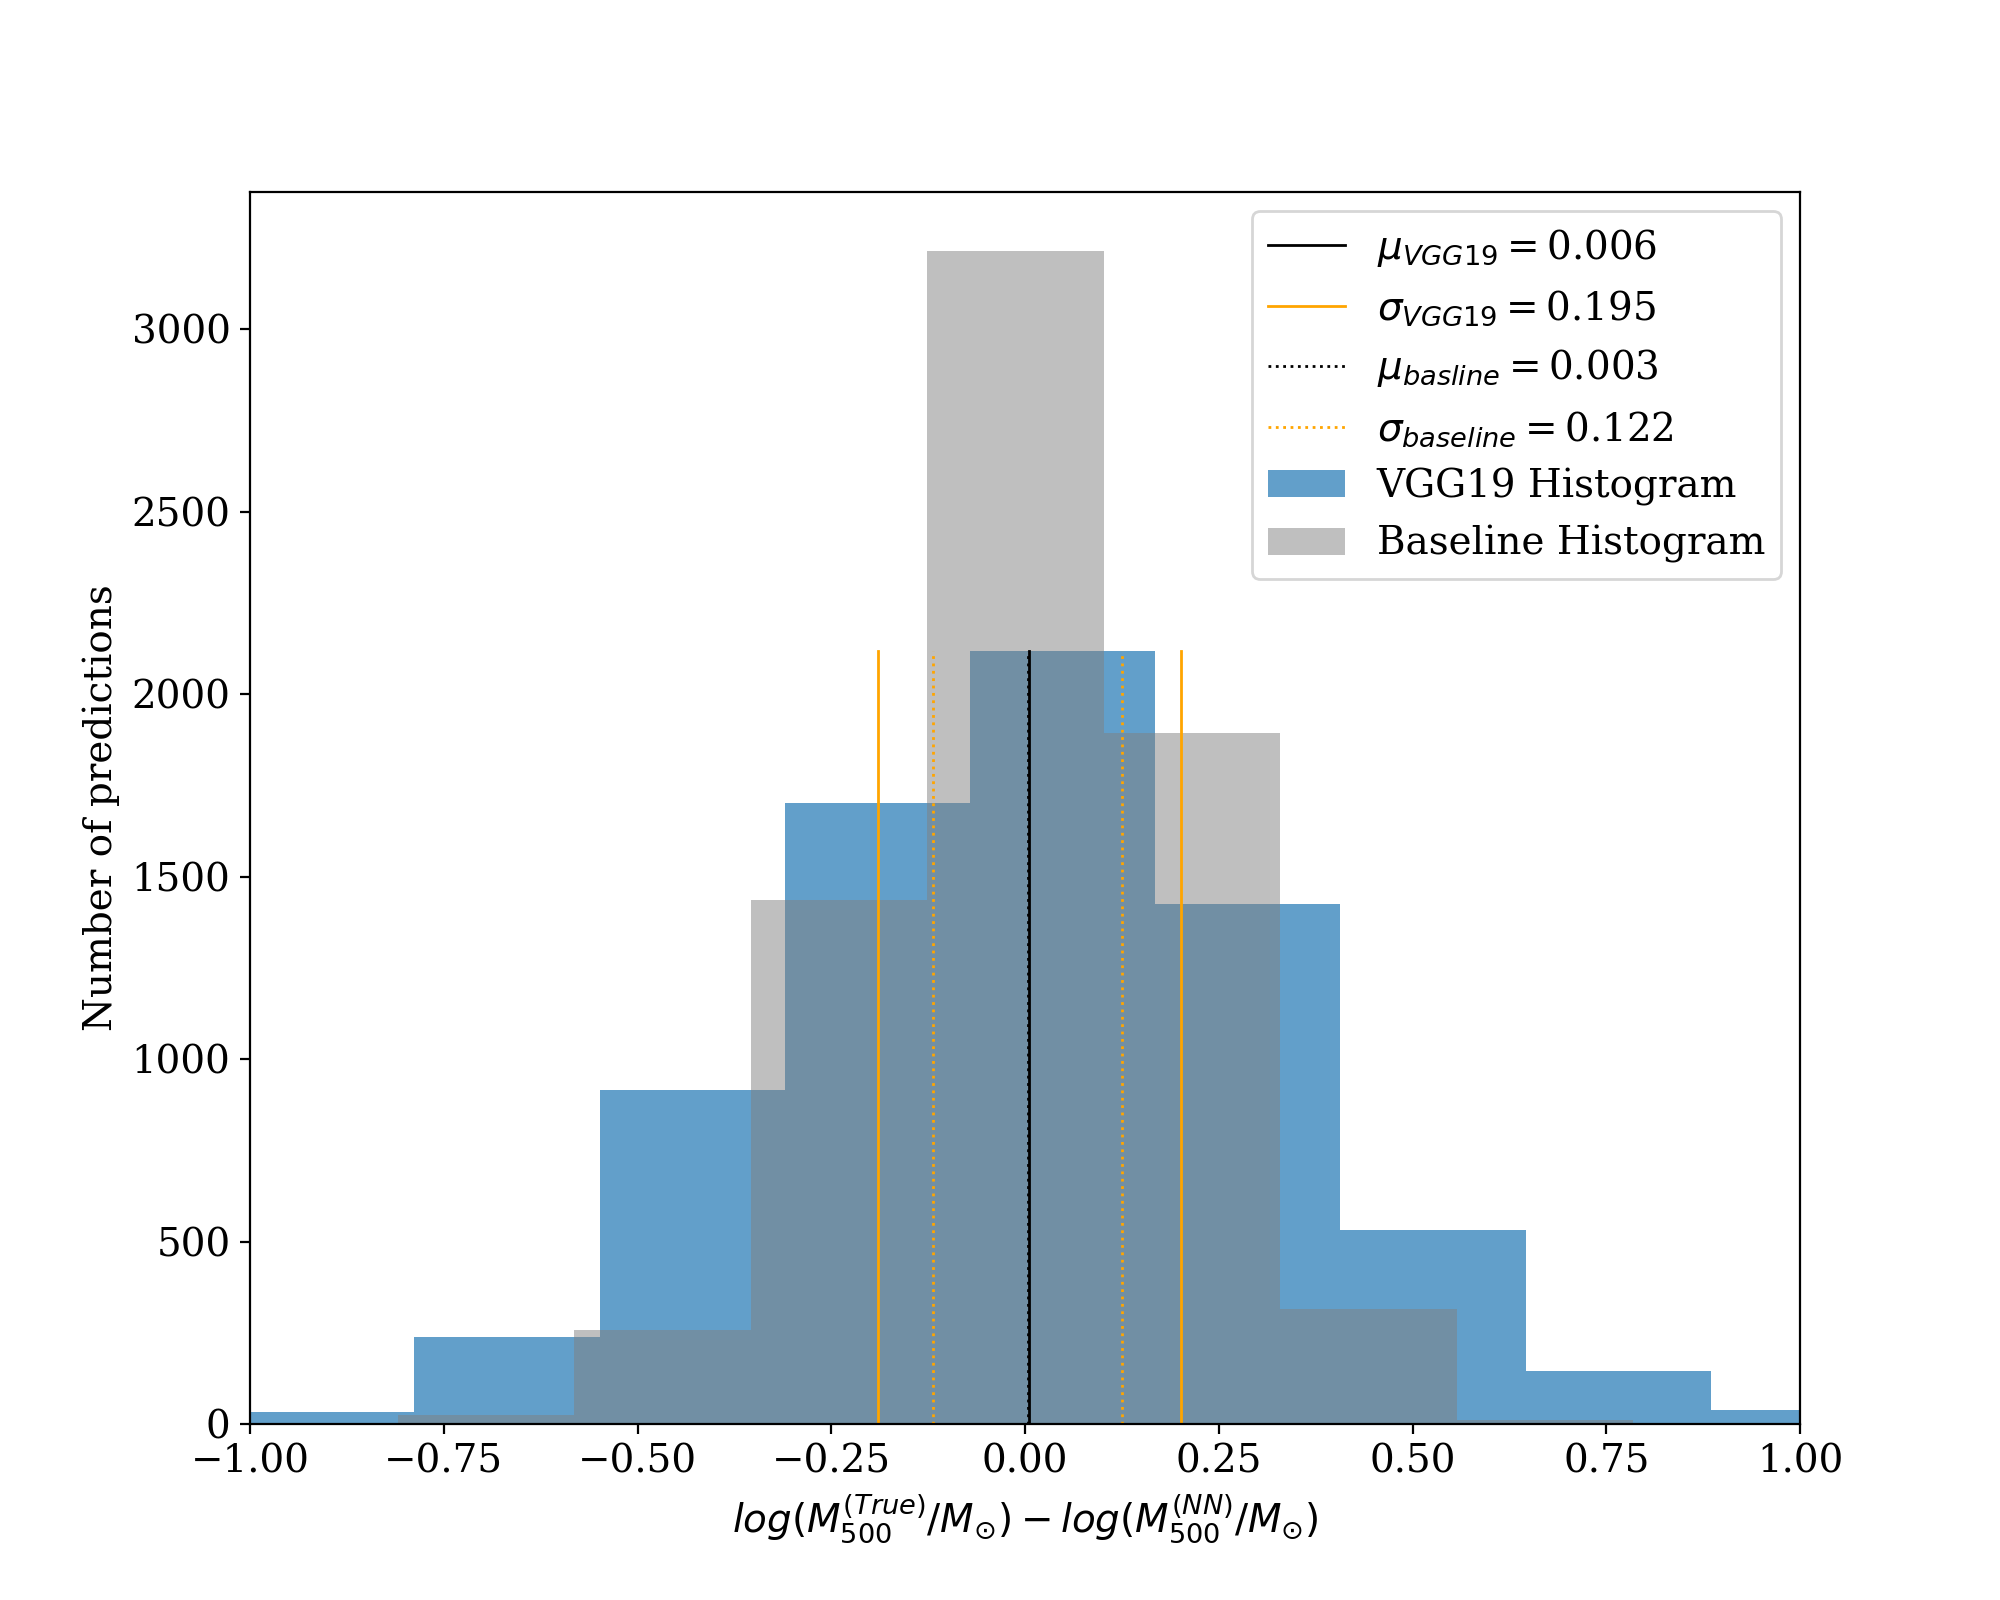
\includegraphics[width=\linewidth]{images/Chapter4/Results/training_VGG19_hist.png}
    \label{fig:training_VGG19_hist}
    \caption{VGG19}
\end{subfigure}
\begin{subfigure}{.325\textwidth}
    \centering
    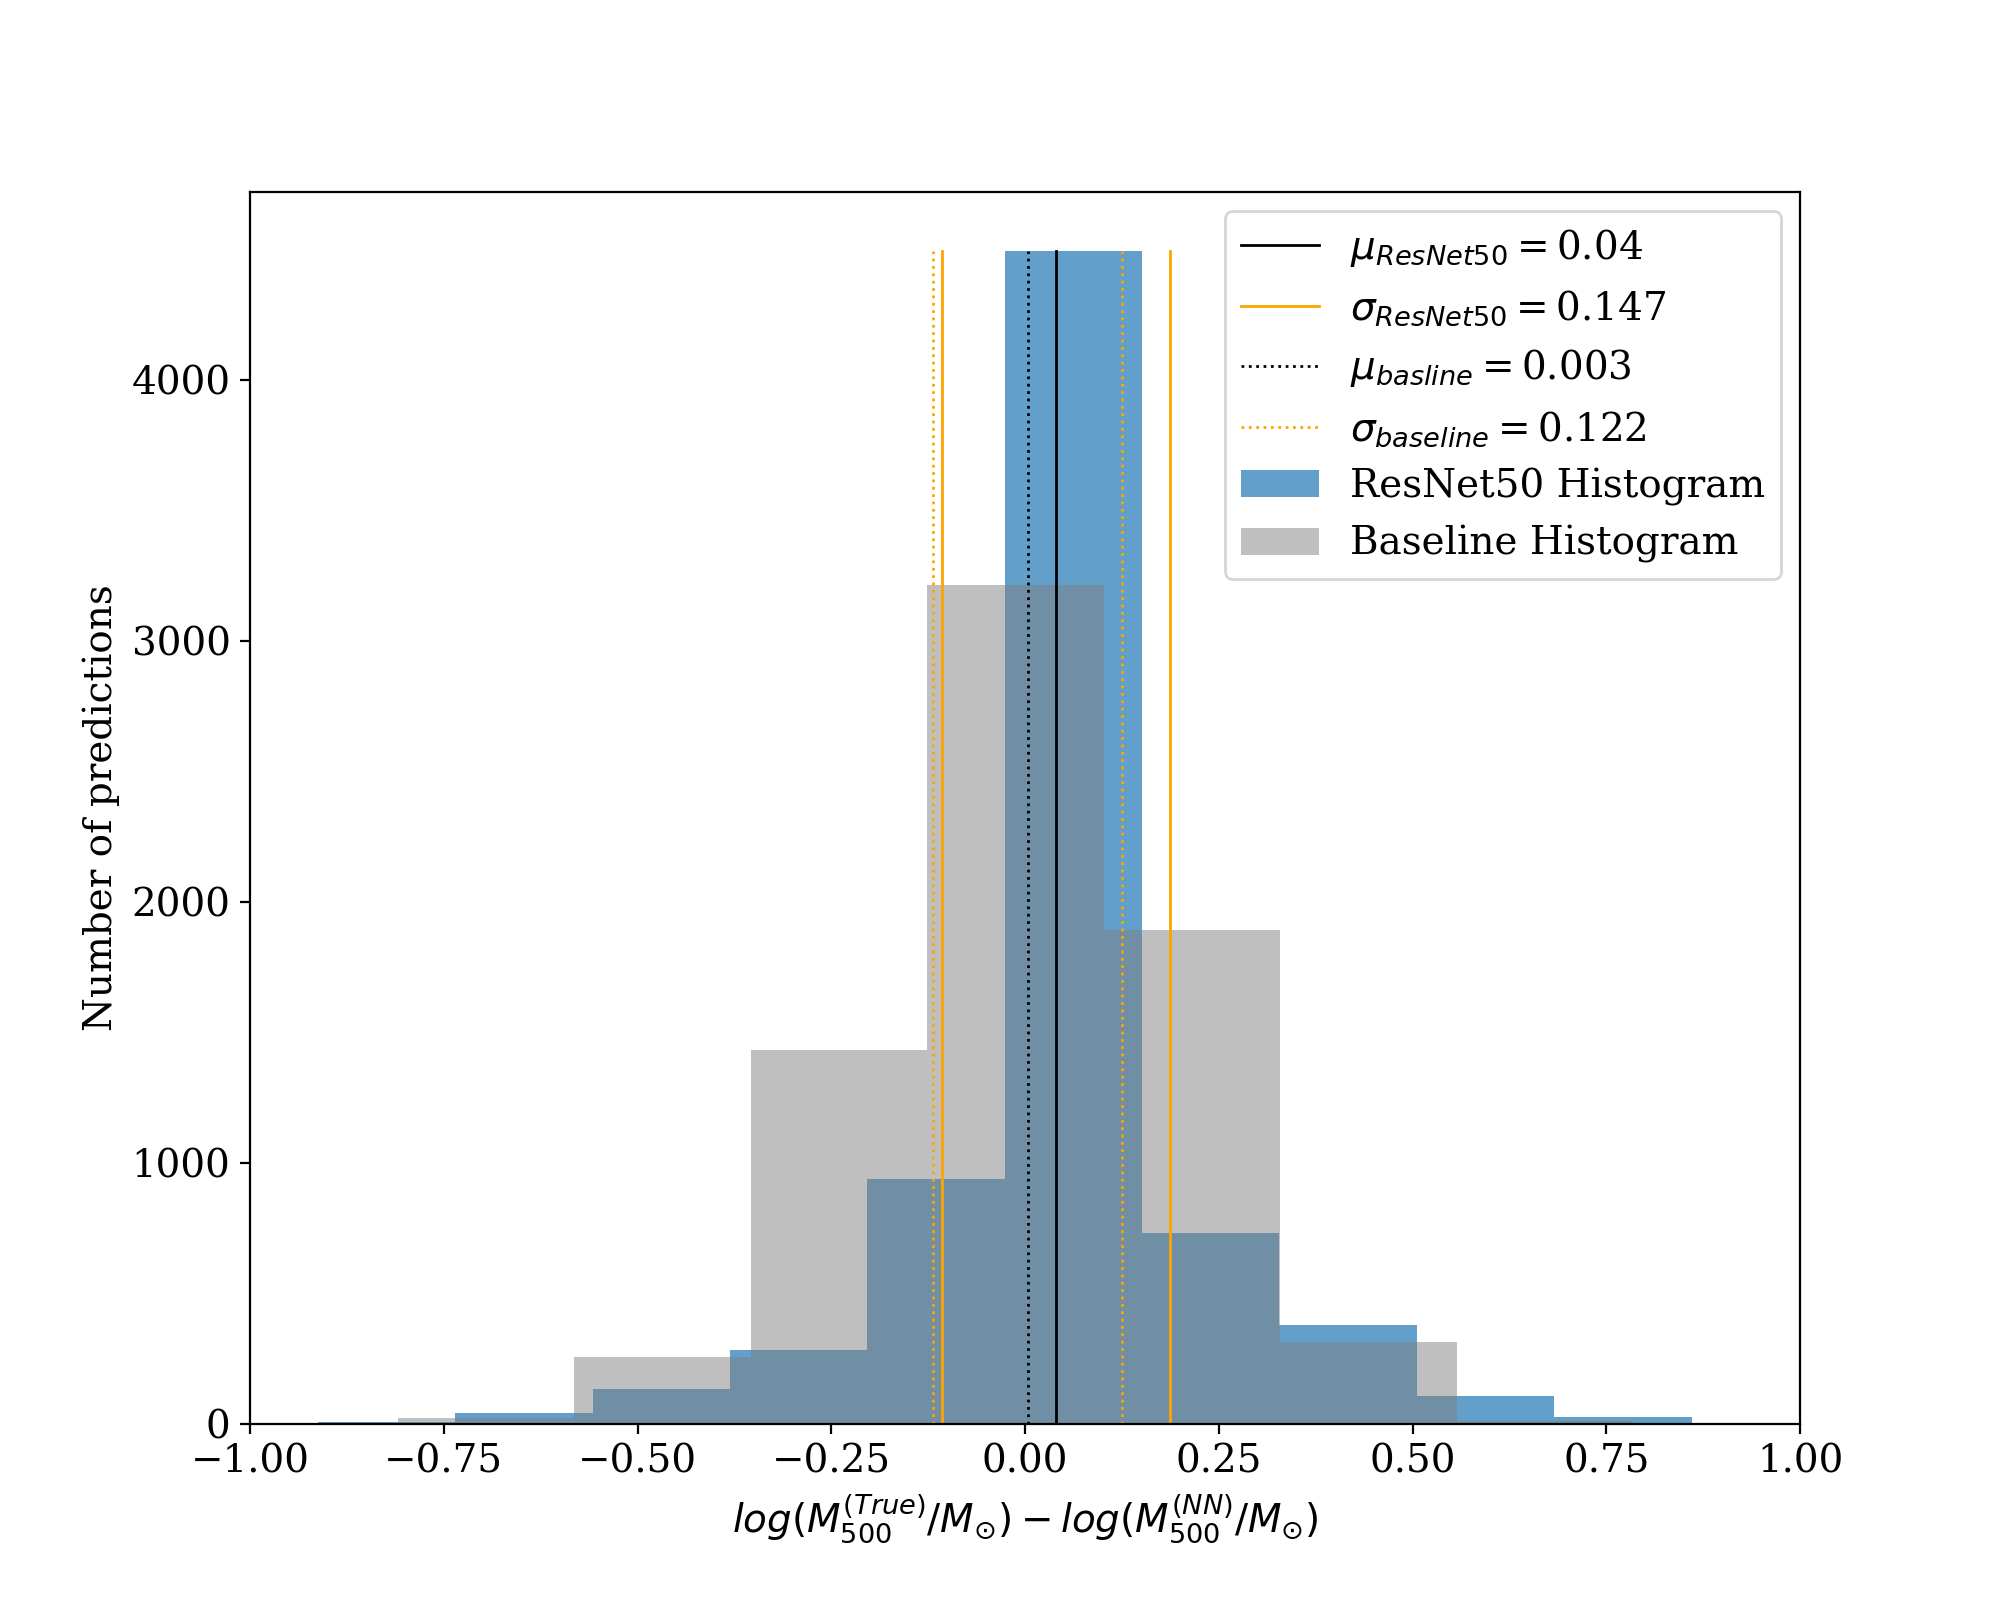
\includegraphics[width=\linewidth]{images/Chapter4/Results/training_ResNet50_hist.png}
    \label{fig:training_ResNet50_hist}
    \caption{ResNet50}
\end{subfigure}
\begin{subfigure}{.325\textwidth}
    \centering
    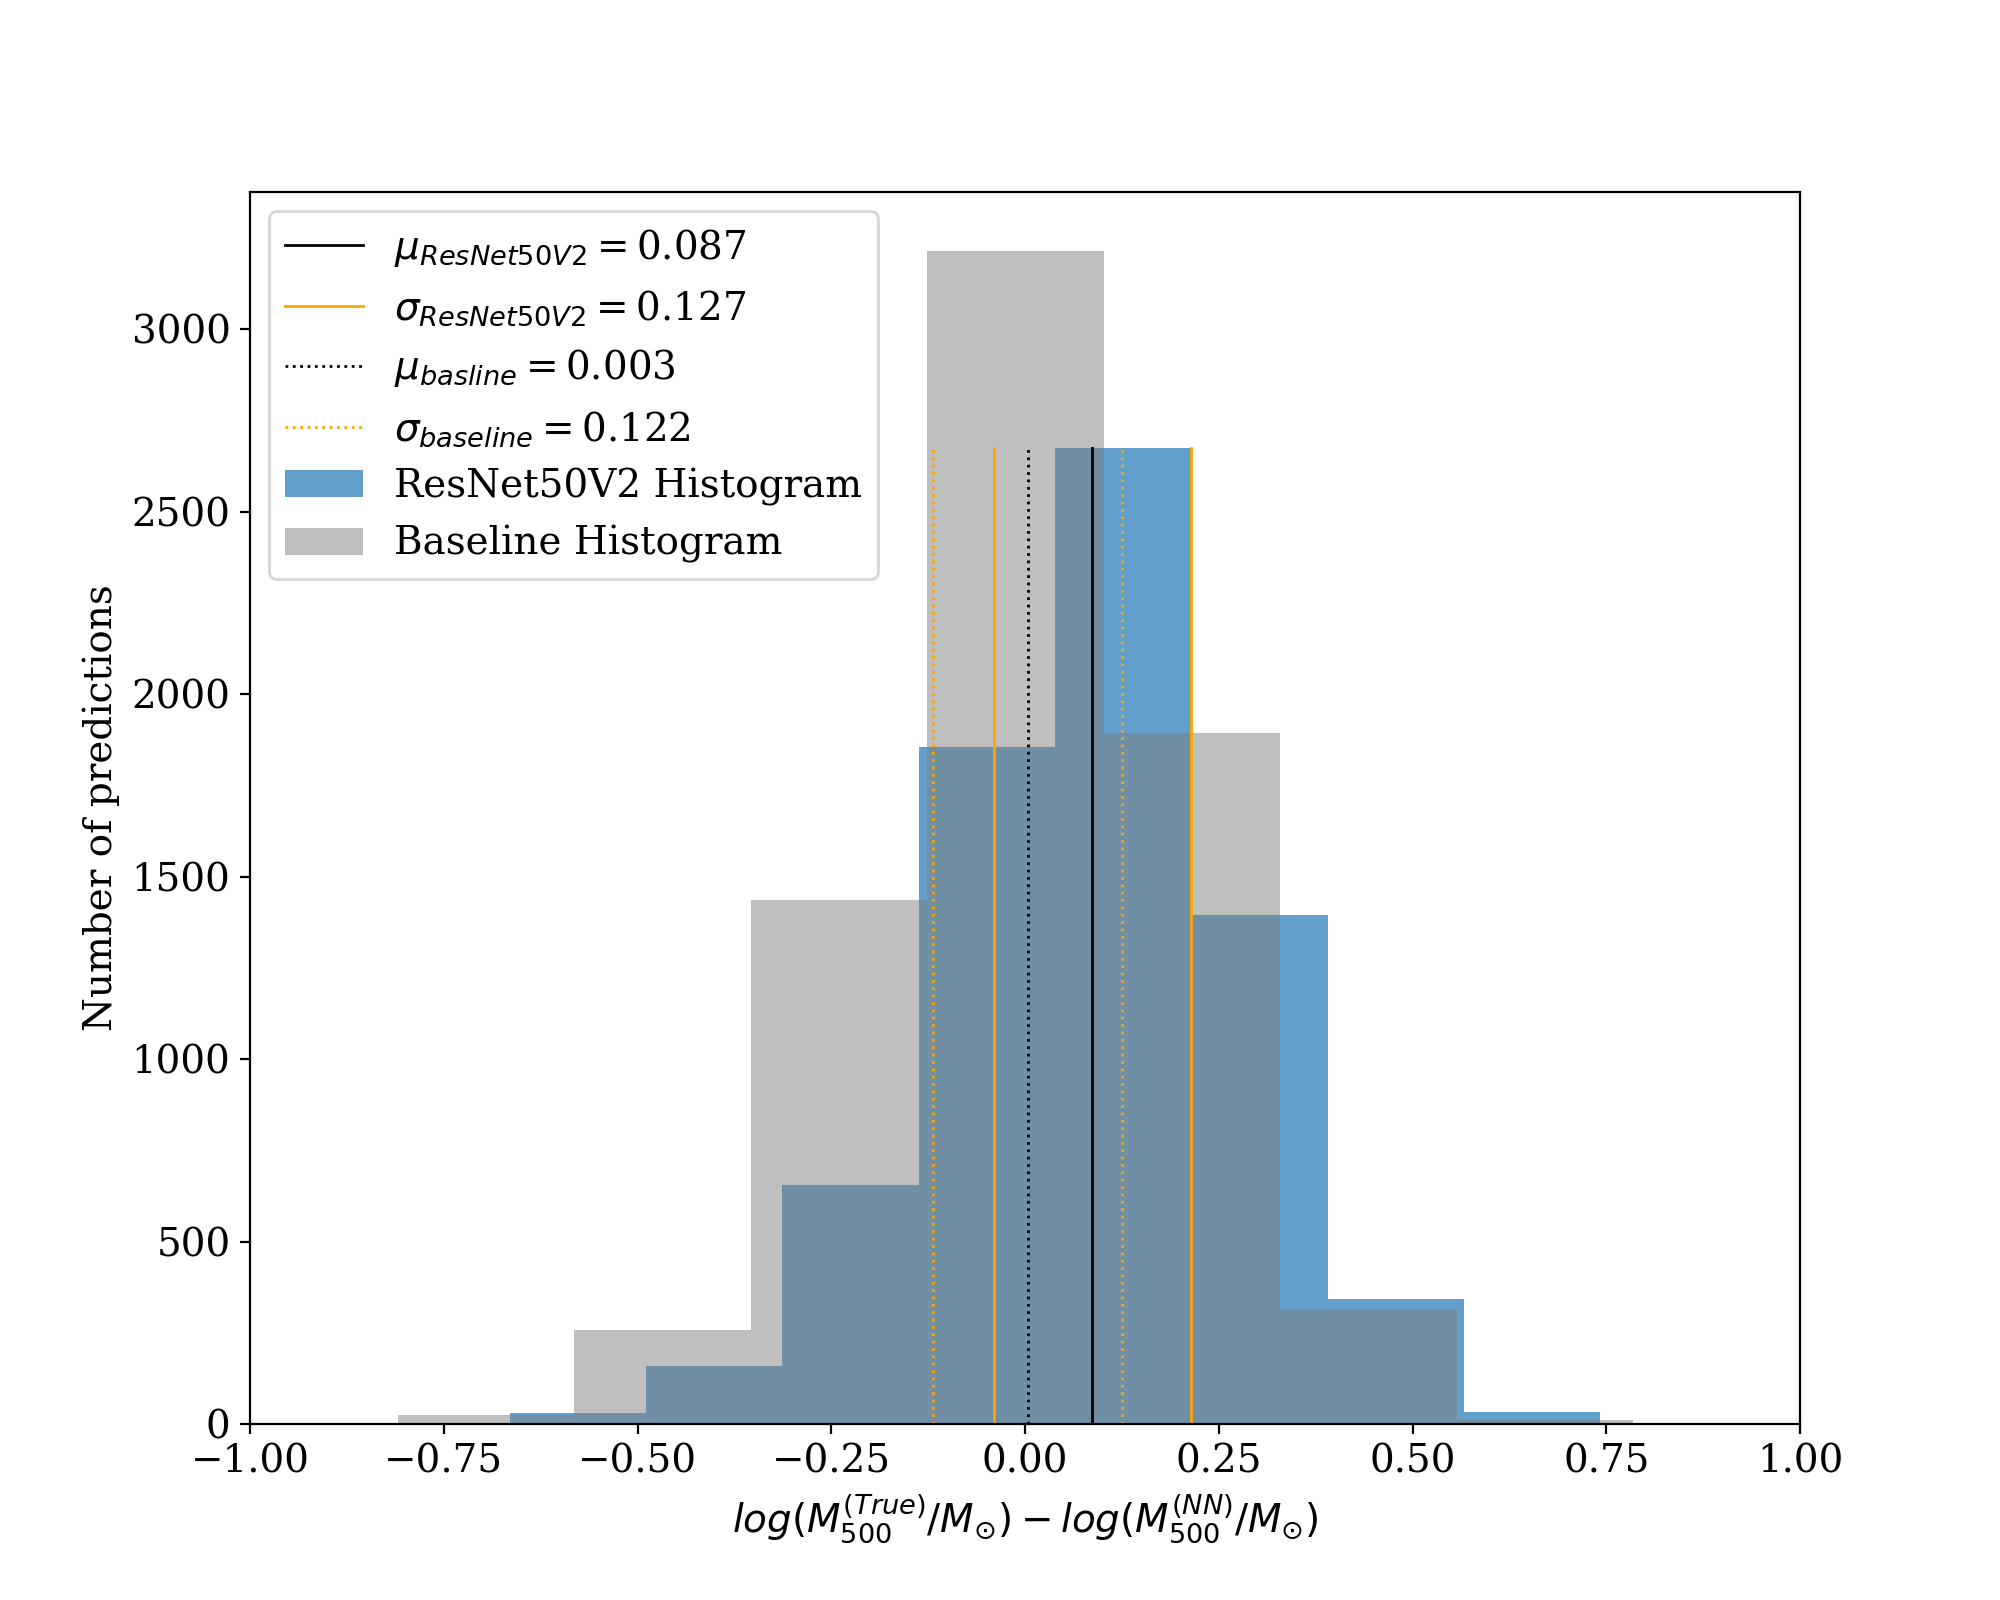
\includegraphics[width=\linewidth]{images/Chapter4/Results/training_ResNet50V2_hist.png}
    \label{fig:training_ResNet50V2_hist}
    \caption{ResNet50V2}
\end{subfigure}
\begin{subfigure}{.325\textwidth}
    \centering
    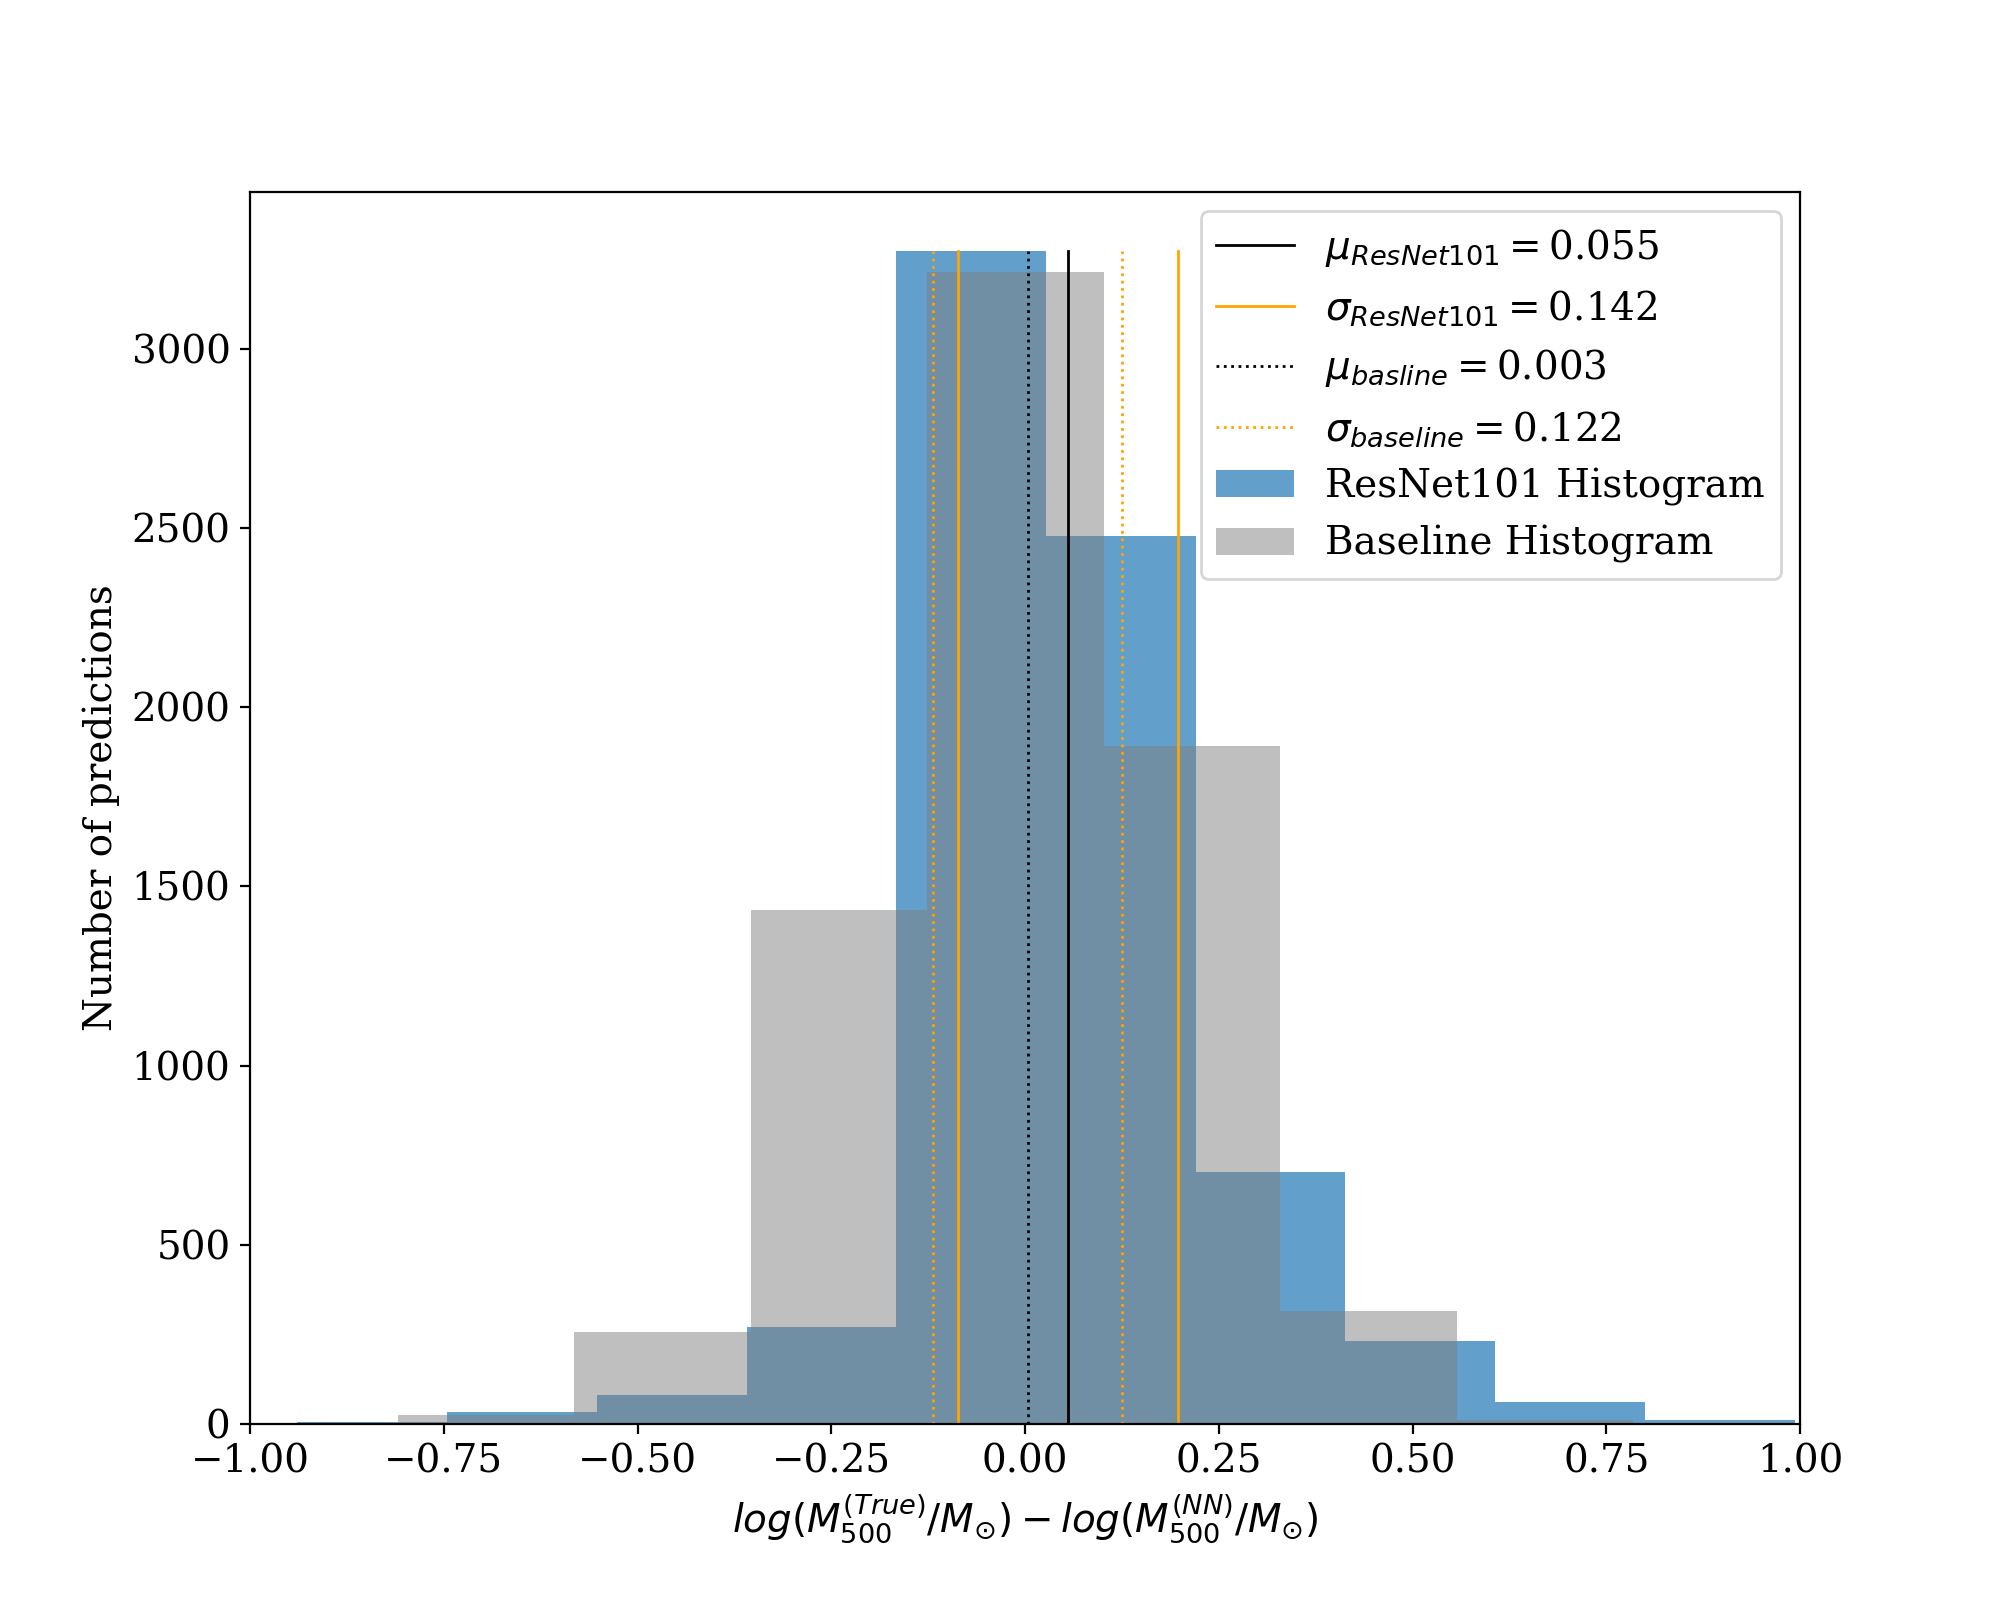
\includegraphics[width=\linewidth]{images/Chapter4/Results/training_ResNet101_hist.png}
    \label{fig:training_ResNet101_hist}
    \caption{ResNet101}
\end{subfigure}
\begin{subfigure}{.325\textwidth}
    \centering
    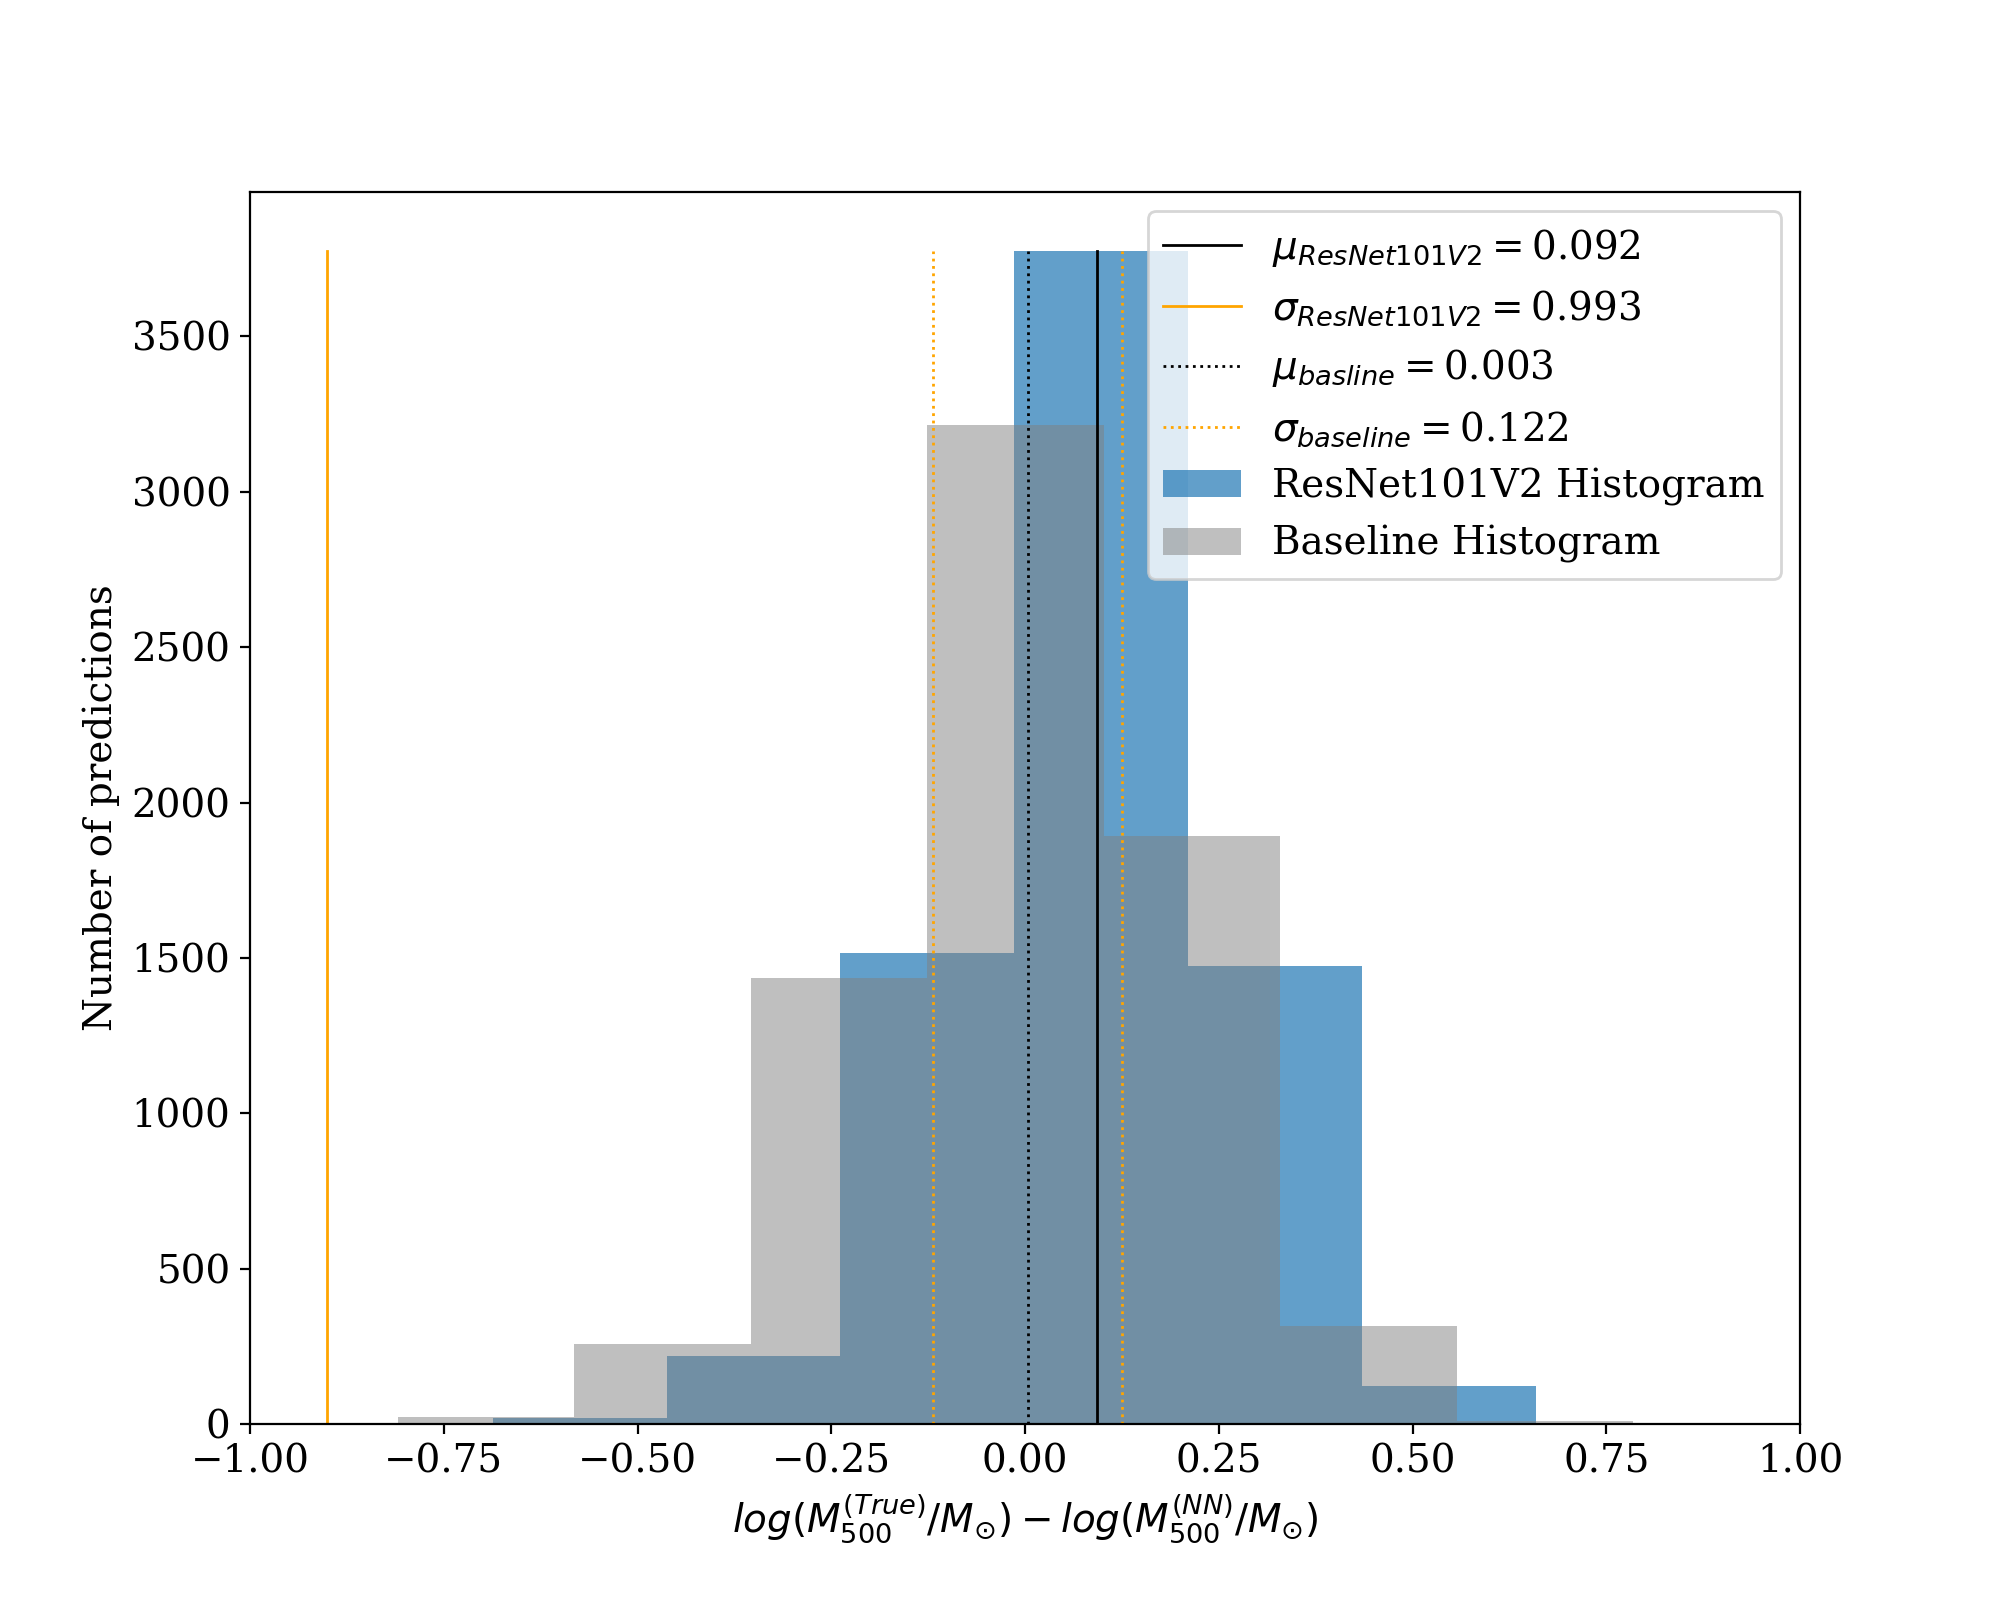
\includegraphics[width=\linewidth]{images/Chapter4/Results/training_ResNet101V2_hist.png}
    \label{fig:training_ResNet101V2_hist}
    \caption{ResNet101V2}
\end{subfigure}
\begin{subfigure}{.325\textwidth}
    \centering
    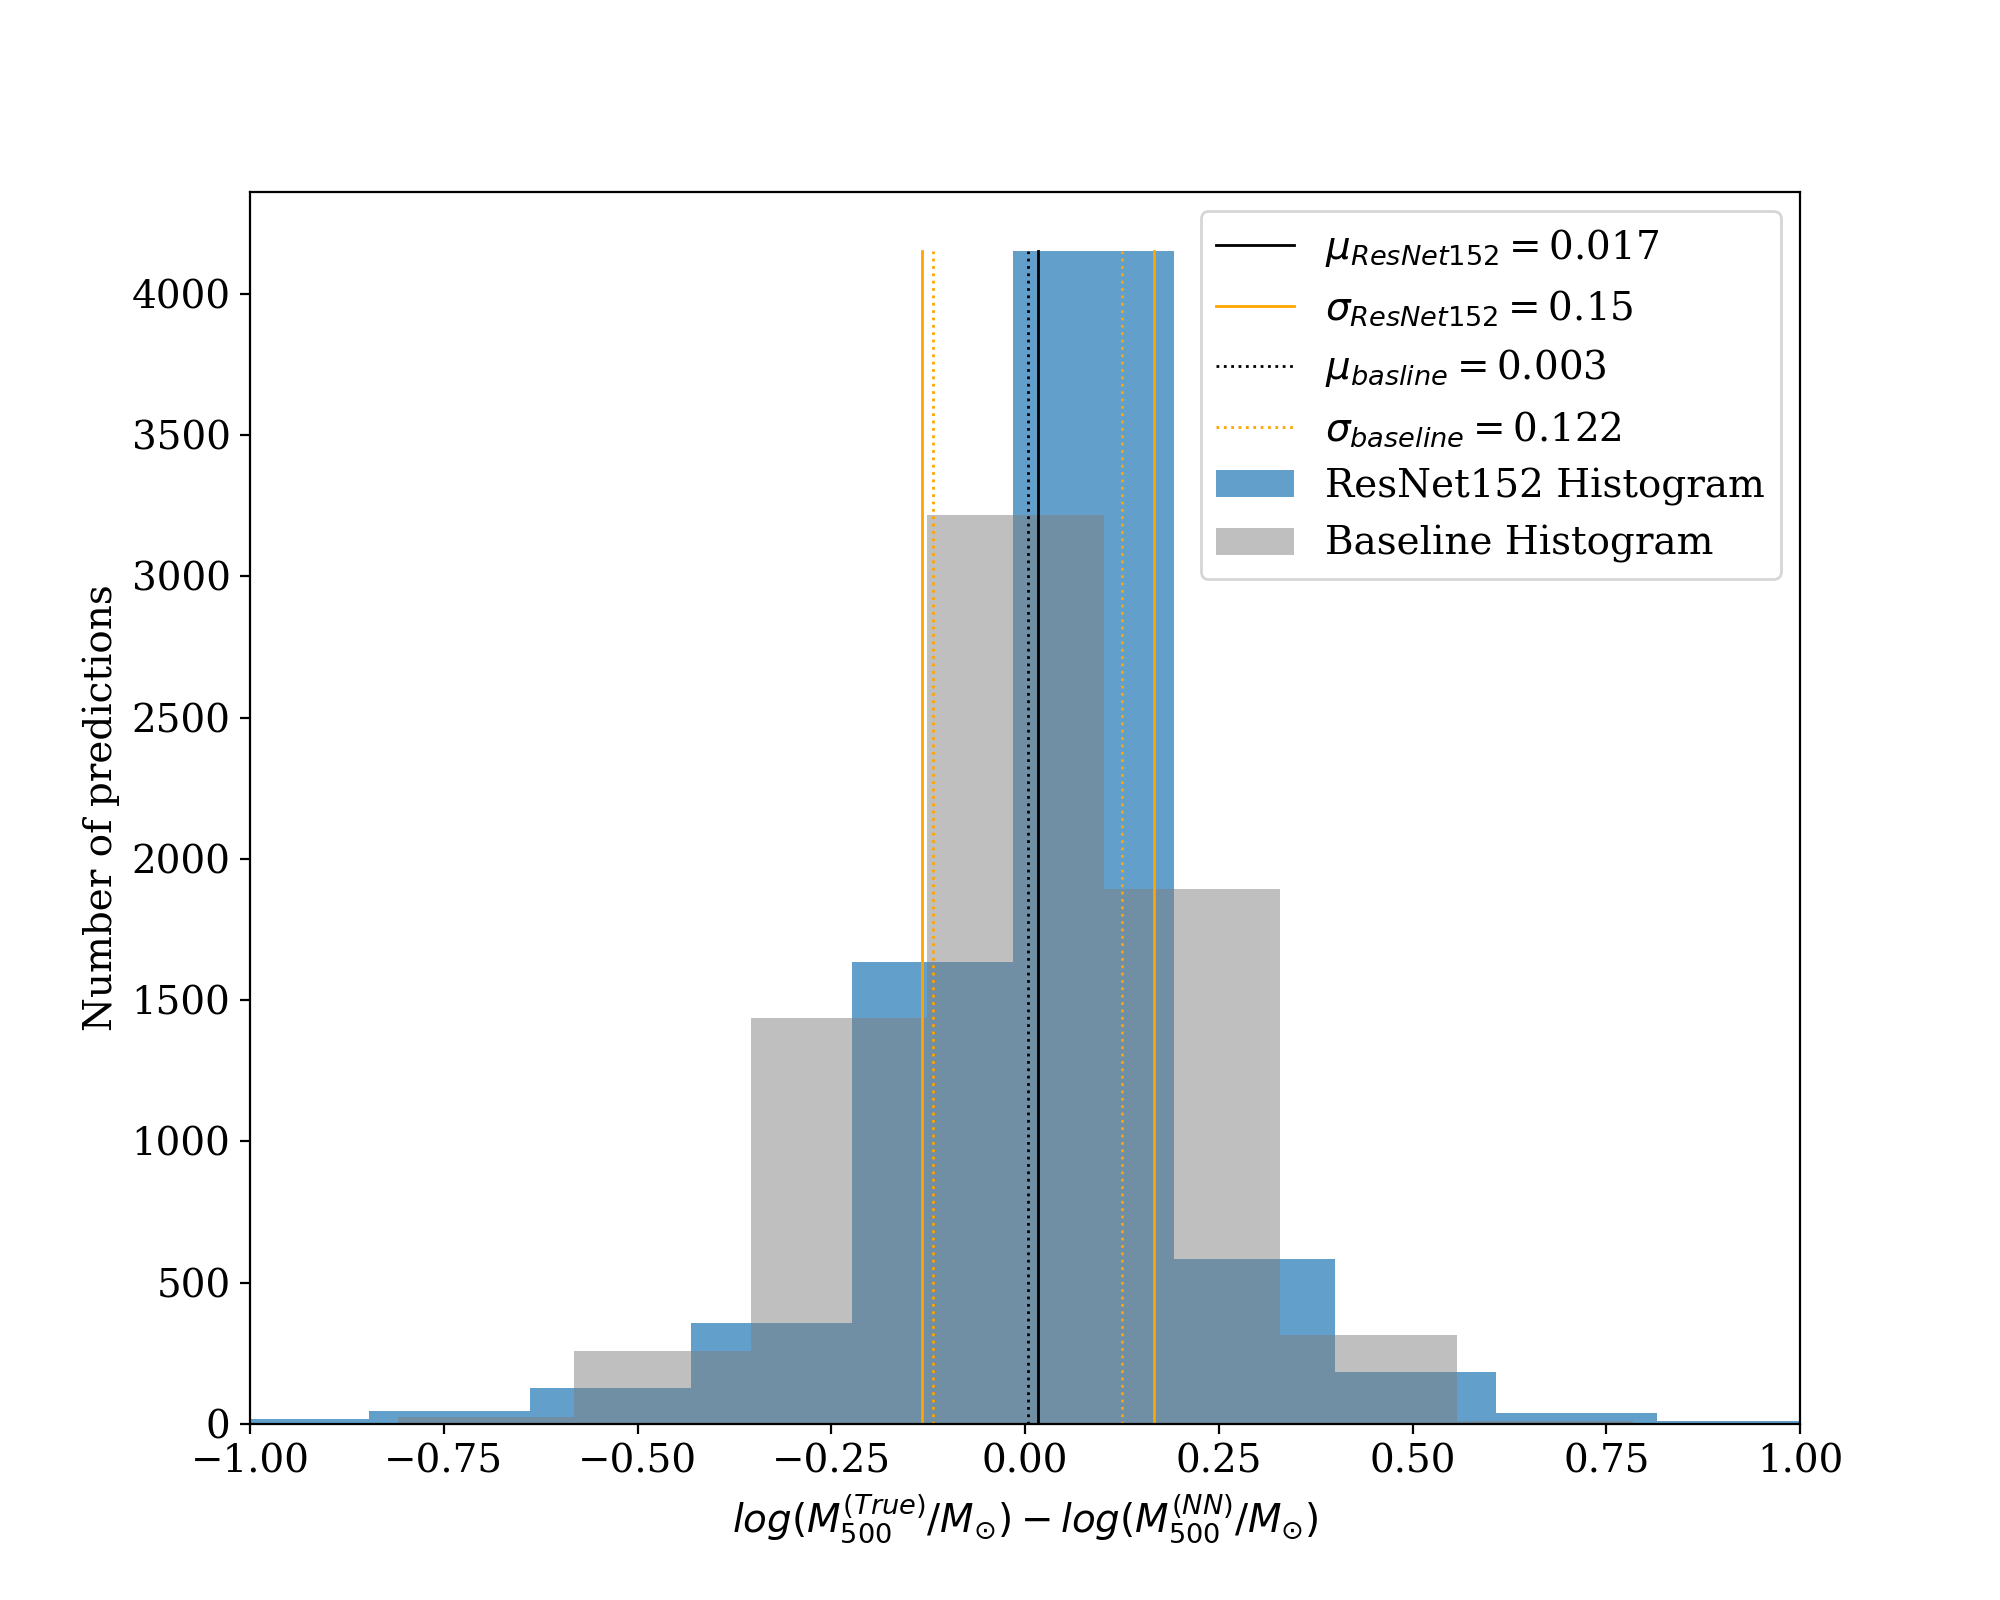
\includegraphics[width=\linewidth]{images/Chapter4/Results/training_ResNet152_hist.png}
    \label{fig:training_ResNet152_hist}
    \caption{ResNet152}
\end{subfigure}
\begin{subfigure}{.325\textwidth}
    \centering
    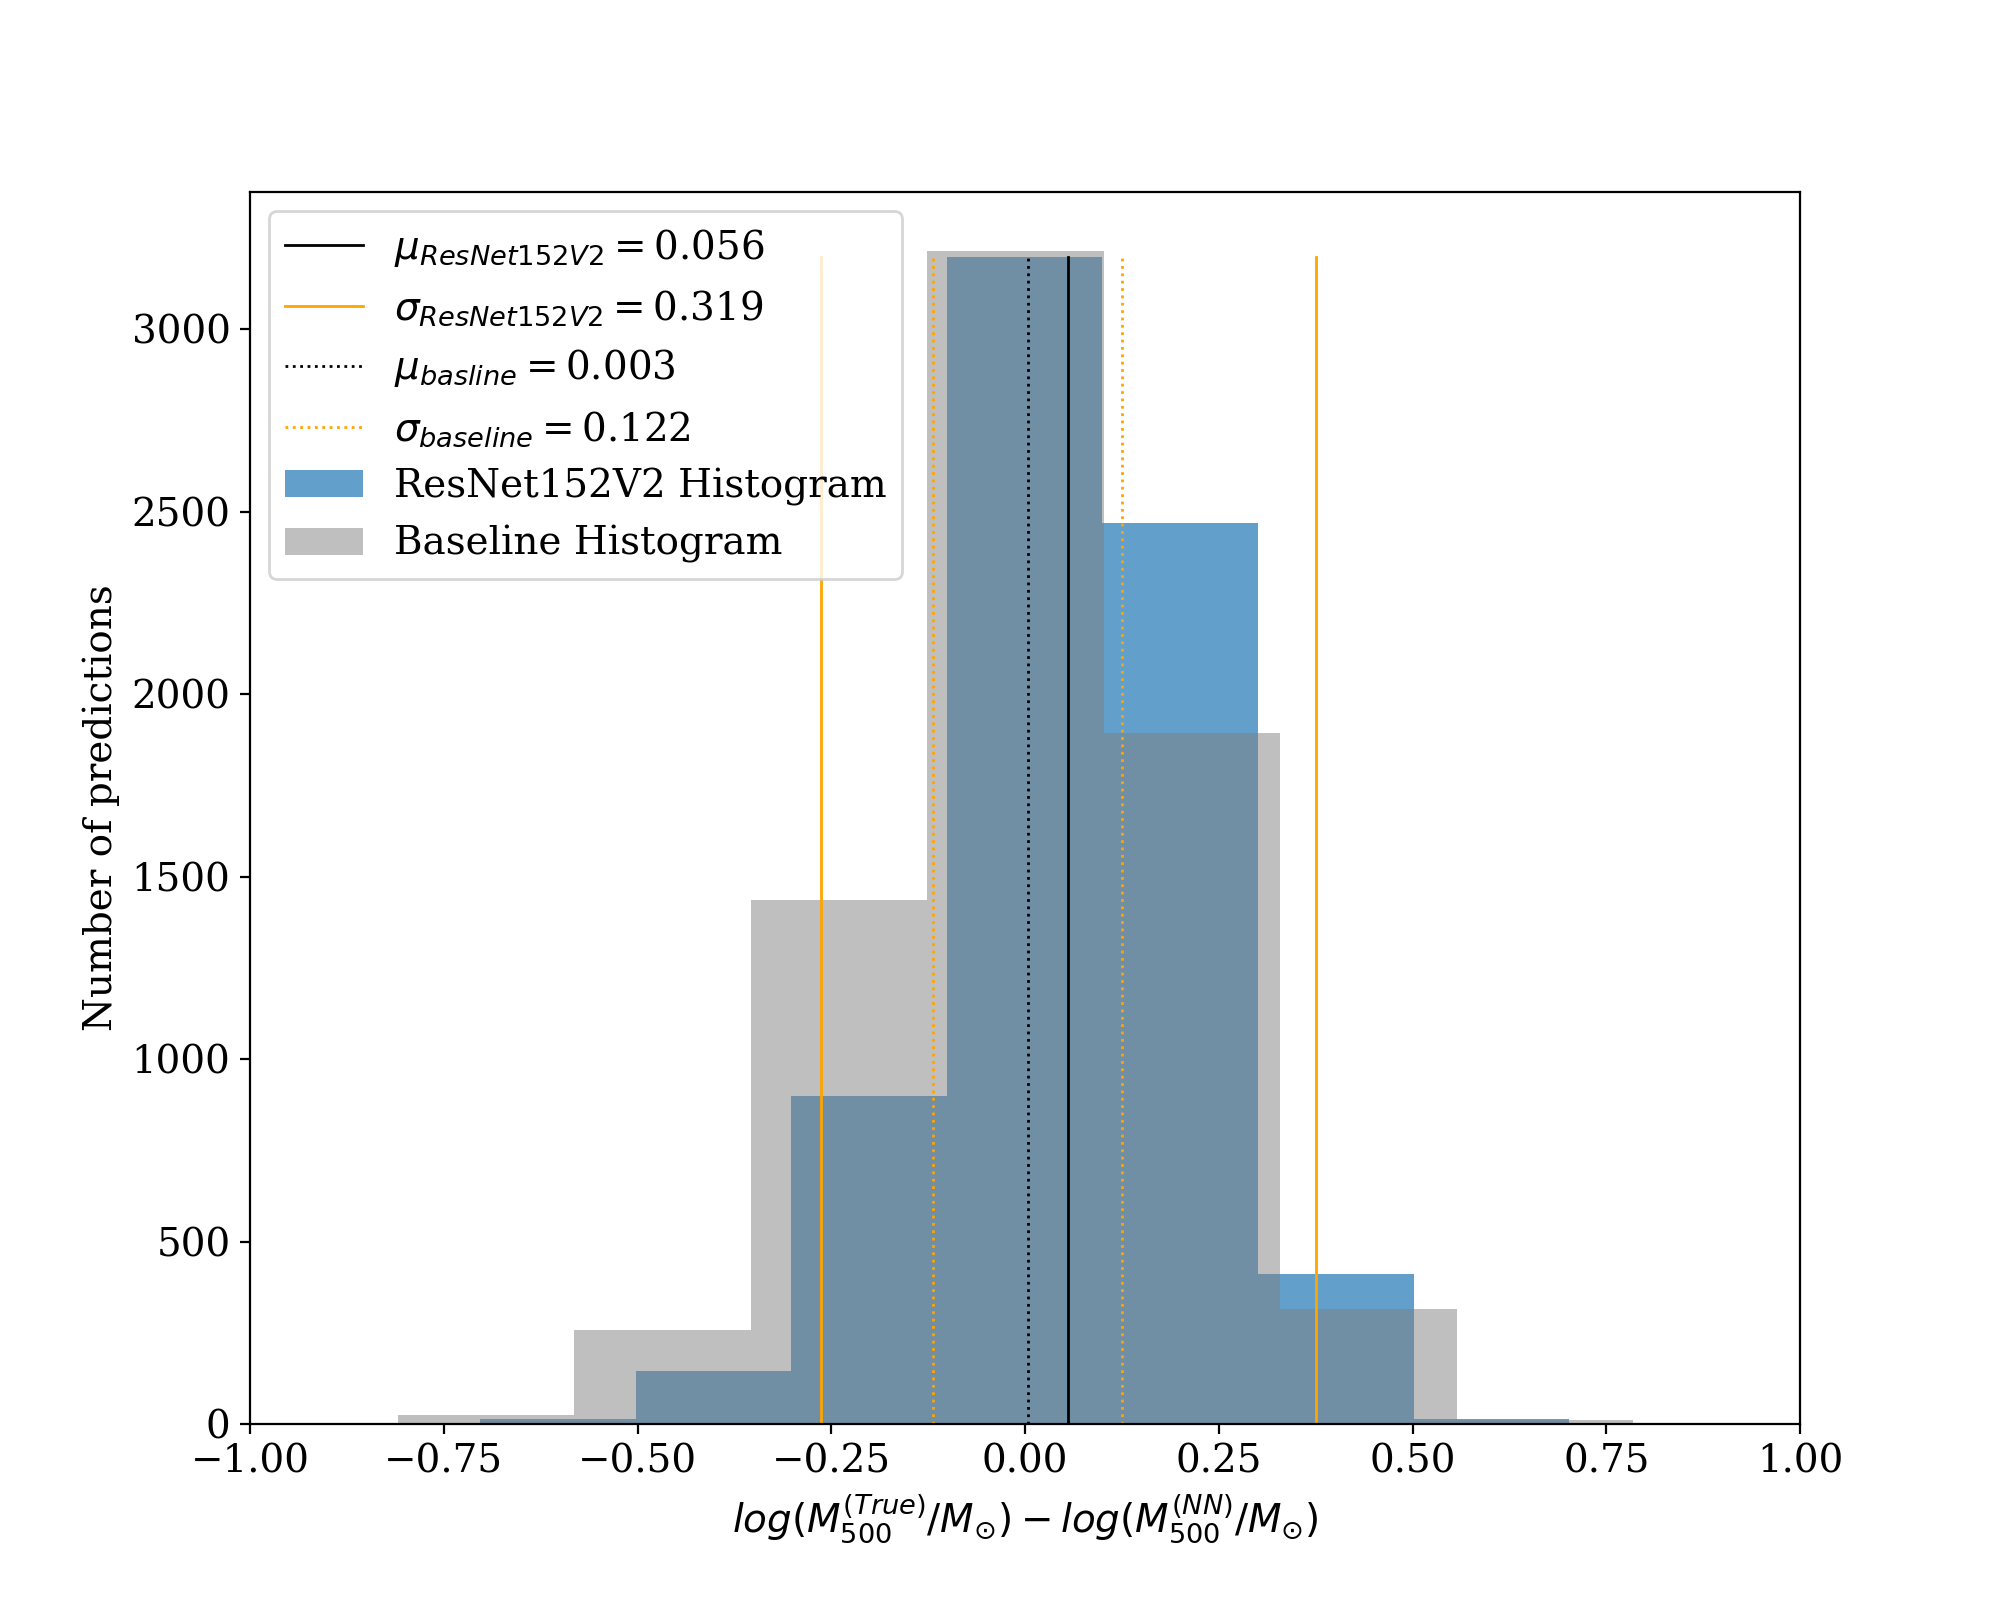
\includegraphics[width=\linewidth]{images/Chapter4/Results/training_ResNet152V2_hist.png}
    \label{fig:training_ResNet152V2_hist}
    \caption{ResNet152V2}
\end{subfigure}
\begin{subfigure}{.325\textwidth}
    \centering
    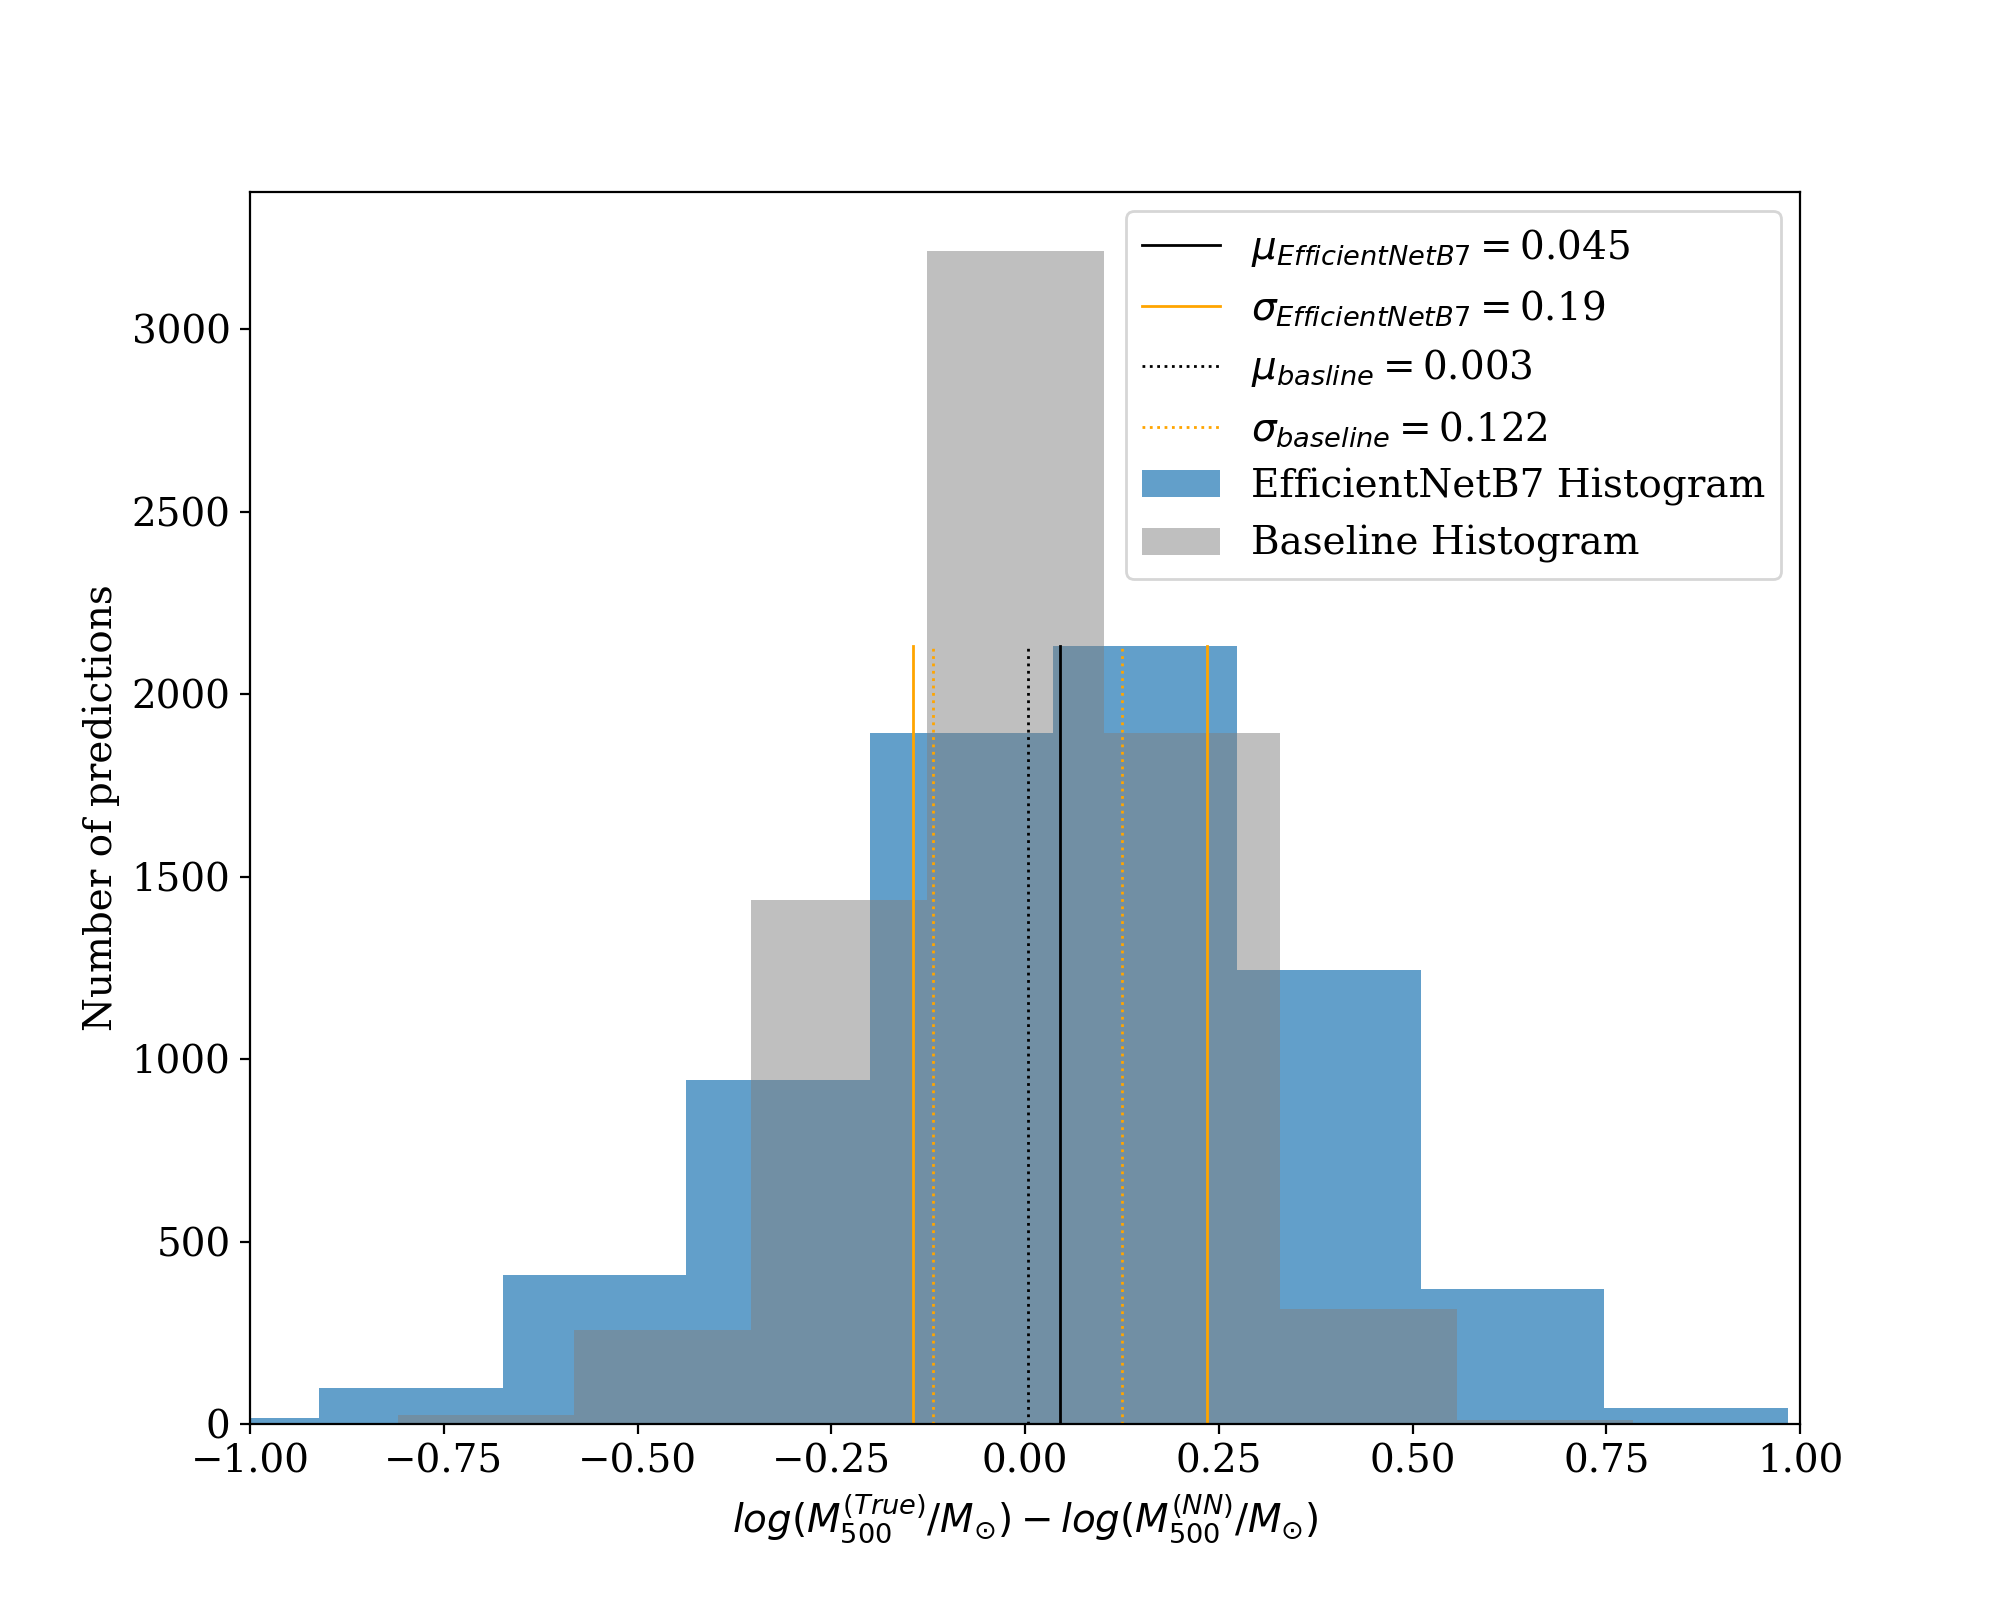
\includegraphics[width=\linewidth]{images/Chapter4/Results/training_EfficientNetB7_hist.png}
    \label{fig:training_EfficientNetB7_hist}
    \caption{EfficientNetB7}
\end{subfigure}
\caption{Comparison histograms between each deep model's best predictions (\textit{blue}) and the best predictions from the basic CNN (\textit{grey}) on the training set.}
\end{figure}